
\documentclass[12pt]{report}
\usepackage{amsmath}
\usepackage{bm}
\usepackage{url}
\usepackage{graphicx} % Required for inserting images
\usepackage{placeins}
\usepackage{geometry}
\usepackage{tcolorbox}
\usepackage{xcolor}
\usepackage{booktabs}
\usepackage{tabularx}
\usepackage{longtable}
% Notes to the authors, removed before release
\newcommand{\authornote}[1]{\textcolor{red}{[#1]}}

 \geometry{
 a4paper,
 left=30mm,
 top=30mm,
 }

\usepackage{cite}
\usepackage{natbib}
\bibliographystyle{plainnat}

\title{Sediment Source Assessment Tool, version 3 (SedSAT3): User's Manual\\[0.6em]
\large For SedSAT3 version 1.1.8 \authornote{version to be confirmed at release}}
\author{Arash Massoudieh
    \and
    Allen C. Gellis
    \and
    Cara L Peterman-Phipps }
\date{Draft, October 2026 \authornote{publication date to be set at release}}
\renewcommand{\theequation}{\arabic{chapter}.\arabic{section}.\arabic{equation}}
\renewcommand{\bibname}{References}
\begin{document}
\sloppy
\setlength{\emergencystretch}{3em}


\maketitle

\section*{Executive Summary}
The Sediment Source Assessment Tool3 (SedSAT3) User’s Manual provides comprehensive guidance for users of the SedSAT3 software, a tool developed for sediment source fingerprinting. SedSAT3 is an update to the earlier version of SedSAT \citep{gormansanisaca2017determining}. The software facilitates the analysis of sediment sources and their contributions to a particular target site by utilizing elemental composition data. Key functions of SedSAT3 include data preparation, statistical analysis, and sediment source attribution using Levenberg--Marquardt maximum likelihood estimation and Bayesian inference by Markov chain Monte Carlo (MCMC) sampling. The manual outlines the steps required for importing and preparing raw data, followed by pre-analysis tasks like correlation matrix generation, outlier detection, and organic matter and particle size corrections. It also provides tools for advanced statistical analysis, including variance analysis and discriminant function analysis, to aid in selecting the most effective elements for fingerprinting. The manual culminates in detailed instructions for executing source attribution models and performing uncertainty analysis. A mathematical appendix explains the theoretical foundations for the modeling methods used in the software, offering users both practical and technical insights for sediment fingerprinting.   
\tableofcontents
\listoffigures




\chapter{Getting started}\label{chap:getting-started}

\section{Installing and running SedSAT3}\label{sec:installing}
SedSAT3 is distributed through its U.S. Geological Survey software release \authornote{repository URL and DOI to be added at release}. The release provides a portable Windows package and the source code.

\paragraph{Windows (portable package).} The portable package needs no installer and no administrator rights.
\begin{enumerate}
    \item Download \texttt{SedSAT3-<version>-windows-x64-portable.zip} from the release page.
    \item Optionally check the download against the SHA-256 checksum published with it, from a Command Prompt:\\ \texttt{certutil -hashfile}\\ \texttt{SedSAT3-<version>-windows-x64-portable.zip SHA256}
    \item Unzip it to any folder you can write to, for example your Desktop.
    \item Double-click \texttt{SedSat3.exe}.
\end{enumerate}
Keep the \texttt{resources} folder next to the program; SedSAT3 reads its tool and form definitions from it. To remove SedSAT3, delete the folder.

\paragraph{Linux and macOS.} SedSAT3 is built from the source code with Qt~6, Armadillo and GSL. The \texttt{README} file in the repository lists the prerequisites and the build commands.

\paragraph{Example data.} The example dataset used throughout this manual, \texttt{SampleData.xlsx}, is in the \texttt{examples} folder of the repository and of the Windows package.

\paragraph{Command line program.} SedSAT3 also includes a command line program, \texttt{sedsat3-cli}, which runs the same analyses from a script file. It has its own manual.

\section{Methods in SedSAT3}\label{sec:methods-table}
SedSAT3 replaces Sed\_SAT \citep{gormansanisaca2017determining}, which was written in R with a Microsoft Access interface. Table~\ref{tab:methods} lists the methods of SedSAT3, where this manual describes them, and how each compares with Sed\_SAT~1.0. The comparison is based on the Sed\_SAT~1.0 source code (U.S. Geological Survey software release, \url{https://doi.org/10.5066/F76Q1VBX}) and its report.

\begin{longtable}{>{\raggedright\arraybackslash}p{2.5cm}>{\raggedright\arraybackslash}p{5.0cm}>{\raggedright\arraybackslash}p{6.1cm}}
\caption{Methods in SedSAT3 compared with Sed\_SAT~1.0.}\label{tab:methods}\\
\toprule
Step or tool & SedSAT3 & Sed\_SAT 1.0 \\
\midrule
\endfirsthead
\toprule
Step or tool & SedSAT3 & Sed\_SAT 1.0 \\
\midrule
\endhead
Values below detection & None: every value must be a number; values below detection are replaced by the user before import (Chapter~\ref{chap:raw-data}). & \textit{Not in SedSAT3.} Non-detects in the source data were imputed for each source group by log-ratio expectation maximization or data augmentation (R package zCompositions), from the reporting limits. \\
\addlinespace
Outlier test (Sec.~\ref{sec:outlier}) & Box--Cox transformation chosen with the Kolmogorov--Smirnov statistic; a value is flagged when it is more than N standard deviations from the group mean (N = 3); flagged samples stay included until the user excludes them. & \textit{Changed.} Same rule (mean $\pm$ N standard deviations, N = 3), but on a transformation chosen with the Shapiro--Wilk test from Tukey's ladder of powers; flagged samples were excluded by default and the user could include them again. \\
\addlinespace
Organic matter and particle size correction (Sec.~\ref{sec:sizeandorganiccorrection}) & One linear or power-law multiple regression on organic matter and particle size, per element and source group; terms applied when significant (p-value) or chosen by the user; isotopes not corrected by default; the correction is for each target sample. & \textit{Changed.} One variable at a time and in sequence: particle size first, then organic content on the size-corrected data. Linear regression on transformed variables (Tukey's ladder), accepted on the slope p-value, $R^2$ and the normality of the residuals, with a bias-correction factor. The correction was relative to the mean of the target samples selected for the run. Stable isotopes were not corrected for organic content (in SedSAT3 they are not corrected by default, for either variable). \\
\addlinespace
Bracket test (Sec.~\ref{sec:bracketing}) & A target value fails when it is above every source sample or below every one; every target sample at once. & \textit{Changed.} The range of all source samples was widened by a tolerance (default 10\%) before the test. \\
\addlinespace
Tracer selection (Sec.~\ref{sec:multiway-dfa}, \ref{sec:dfa-tools}) & Forward stepwise discriminant function analysis: multi-way, one vs.\ one, one vs.\ the rest; the constituents up to the smallest $\chi^2$ p-value are selected; leave-one-out confusion matrix of the source samples. & \textit{Similar.} Forward stepwise discriminant function analysis among all groups, adding tracers by Wilks' $\Lambda$ with an entry significance level (default 0.01; R package klaR), with the same leave-one-out confusion matrix. It also computed tracer weighting factors from each tracer's classification rate, which SedSAT3 does not use. \\
\addlinespace
Other tracer screening (Sec.~\ref{sec:tools-selection}, \ref{sec:tools-exploration}) & Analysis of variance, auto-select (pairwise t-tests), discriminant power, correlation matrix. & \textit{New in SedSAT3.} Sed\_SAT~1.0 tested the assumptions of the DFA instead: multivariate normality (Shapiro--Wilk, Mardia, Royston, Henze--Zirkler) and equal dispersion, choosing raw or Box--Cox transformed data for the DFA. \\
\addlinespace
Distributions (Sec.~\ref{sec:tools-exploration}) & Distribution fitting, Kolmogorov--Smirnov tests, optimal Box--Cox parameters. & \textit{New in SedSAT3.} Sed\_SAT~1.0 used the Shapiro--Wilk test to choose transformations. \\
\addlinespace
Isotopes (Sec.~\ref{sec:stable-isotopes}) & $\delta$ values enter the mass balance through the base element's content. & \textit{Changed.} $\delta$ values were mixed as ordinary tracers; marking a tracer as an isotope only kept it out of the imputation and the organic content correction. \\
\addlinespace
Deterministic fingerprinting (Sec.~\ref{sec:lmmle}, \ref{sec:fingerprinting-batch}) & Maximum likelihood with log-normal errors (Levenberg--Marquardt), one target sample or a batch. & \textit{Changed.} Minimized the sum of squared relative errors between the target and the mixture of source means, optionally weighted by the DFA weighting factors (Nelder--Mead optimization), for each target sample. \\
\addlinespace
Bayesian fingerprinting (Sec.~\ref{sec:bayesian_cmb}) & Bayesian chemical mass balance by MCMC, with credible intervals and posterior predictive checks; one target sample or a batch. & \textit{New in SedSAT3.} \\
\addlinespace
Uncertainty and checks (Sec.~\ref{sec:tools-uncertainty}) & Error analysis (realizations with a percentage of the source samples removed at random); source verification (each source sample fingerprinted as a target). & \textit{Changed.} The Monte Carlo analysis removed one randomly chosen sample from each source group per iteration (default 1,000 iterations). Source samples were also fingerprinted as targets, as in source verification. \\
\addlinespace
Program & Stand-alone program for Windows, Linux and macOS; command line program \texttt{sedsat3-cli} for scripts (Sec.~\ref{sec:installing}). & \textit{Changed.} R scripts run from a Microsoft Access interface on Windows. \\
\bottomrule
\end{longtable}

\section{How to read this manual}
Chapter~\ref{chap:raw-data} describes how to prepare and import the data. Chapters~\ref{chap:deterministic} and~\ref{chap:bayesian} follow the menus \textbf{Tools}$\rightarrow$\textbf{Deterministic Sediment Fingerprinting} and \textbf{Tools}$\rightarrow$\textbf{Bayesian Sediment Fingerprinting}, whose numbered steps are the usual order of a sediment fingerprinting study. Chapter~\ref{chap:other-tools} describes the tools under \textbf{Tools}$\rightarrow$\textbf{Other Statistical Tools}, in the order and groups in which the program lists them, and Chapter~\ref{sec:basic_concepts} gives the mathematical basis of the methods. Menu paths are written \textbf{Menu}$\rightarrow$\textbf{Item}, using the names shown by the program.

\subsection{The result window}\label{sec:result-window}
When an analysis finishes, SedSAT3 opens a result window. The window contains one \emph{panel} for each result of the analysis (for example, the p-values, the selected constituents and Wilks' $\Lambda$ of a discriminant function analysis), stacked from top to bottom. When there are more panels than fit in the window, scroll down, or enlarge the window, to see the rest. On the right of each panel are buttons:
\begin{itemize}
    \item the graph button~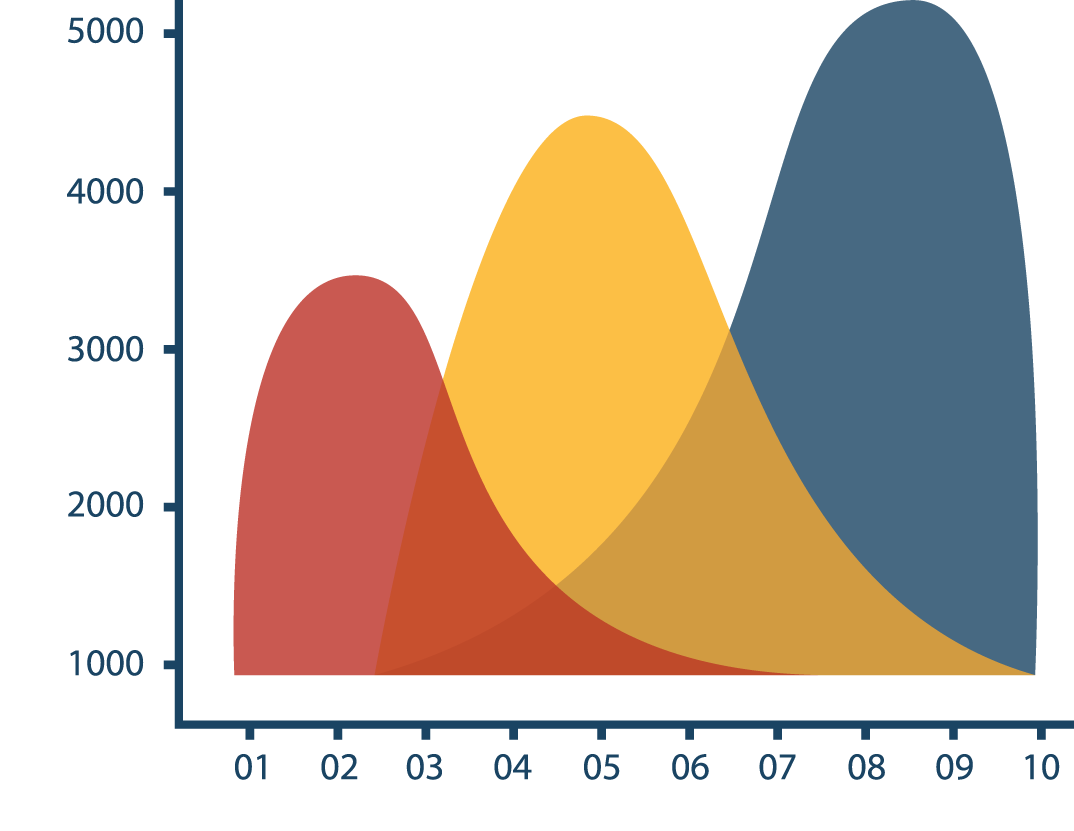
\includegraphics[width=0.5cm]{Figures/Graph.png} shows the result as a chart;
    \item the table button~
\includegraphics[width=0.5cm]{Figures/table.png} shows it as a table, which can be exported to a CSV file;
    \item the export button~
\includegraphics[width=0.5cm]{Figures/export.png} saves it to a text file.
\end{itemize}
Chart windows have an \textbf{Export to PNG} button. Every result also appears in the \textbf{Results} list below the tools, where you can reopen it later; results are saved with the project.

\subsection{Settings shared by many tools}\label{sec:shared-settings}
Many tool forms have the same options:
\begin{itemize}
    \item \textit{Use only selected elements}: use only the constituents marked \textit{Yes} in \textbf{Settings}$\rightarrow$\textbf{Constituent Properties}. When unchecked, the tool uses every element and isotope in the data.
    \item \textit{Use only selected samples}: use only the samples marked \textit{Yes} in \textbf{Settings}$\rightarrow$\textbf{Include/Exclude Samples}.
    \item \textit{OM and Size Correct based on target sample} (or \textit{Apply size and organic matter correction}): run the tool on source data corrected for organic matter and particle size (Section~\ref{sec:sizeandorganiccorrection}) for the target sample named.
\end{itemize}
Each tool applies these options to its own run only; they are not carried from one tool to the next. To compare results, run the tools with the same options. Your selections of constituents and samples, the constituent properties and all results are saved in the project file (\textbf{File}$\rightarrow$\textbf{Save}).

\begin{tcolorbox}[colback=yellow!10,colframe=yellow!50!black,title=Note]
Some tools have the option \textit{Modify the included elements based on the results} (step~4, stepwise discriminant function analysis; analysis of variance; auto-select elements). When it is checked, the tool changes the \textit{Include in analysis} column of \textbf{Settings}$\rightarrow$\textbf{Constituent Properties}: the constituents it does not select are excluded, and they stay excluded for every later tool, including the earlier steps if you run them again (for example, a later bracketing test then shows only the selected constituents). To go back, include the constituents again in \textbf{Settings}$\rightarrow$\textbf{Constituent Properties}. The particle size and organic matter constituents are never changed by these tools.
\end{tcolorbox}

\chapter{Raw data preparation}\label{chap:raw-data}
The raw data for SedSAT3 must be prepared as a single Excel spreadsheet file with multiple tabs. The first tab contains the elemental profiles of the target samples, and each subsequent tab contains the elemental profiles for one source group. In each sheet, each row corresponds to one sample, the first column contains the sample names, and each remaining column represents one element. Grain size and/or organic content may appear in any column. For SedSAT3 to function correctly, the data must be properly formatted; the example dataset \texttt{SampleData.xlsx} (Section~\ref{sec:installing}) shows the layout. The specific text used for column or field headers is not important, but the relative position of columns in the source and target datasets must be identical---this is a core requirement for the program to run successfully. Column or field headers should be unique; no field name may match another field name within the same dataset. Note that each sheet must contain exactly the same elements, named in exactly the same way.

\paragraph{Missing, zero and negative values.} Every cell must contain a finite number. SedSAT3 has no code for a missing value: an empty cell, text, \texttt{NaN} or \texttt{Inf} stops the import with a message giving the sheet, row and column of the cell. A value below the detection limit must therefore be replaced, before import, by a number you choose (for example, a fraction of the detection limit). Zero and negative values are accepted, but:
\begin{itemize}
    \item Elements are modeled on a logarithmic scale (Chapter~\ref{sec:basic_concepts}), so an element with a zero or negative value cannot be used in fingerprinting; the fingerprinting tools stop with a message naming it. Exclude such an element, or correct its values.
    \item Isotopes are entered as $\delta$ values, which are often negative ($\delta^{13}$C) or both positive and negative ($\delta^{15}$N). This is expected: $\delta$ values are used on a linear scale and are never log-transformed (Section~\ref{sec:stable-isotopes}). Give such a constituent the \textit{Isotope} type (Section~\ref{sec:importing_data}).
    \item The Box--Cox transformation (Section~\ref{sec:outlier}) needs positive values. A constituent with a zero or negative value is used untransformed, its $\lambda$ is reported as 1, and the program lists the constituents it left untransformed.
\end{itemize}

\paragraph{Number of samples and source groups.} SedSAT3 needs at least two source groups. Each source group needs at least two samples for its statistics, and more for some tools: the organic matter and particle size regression needs more samples in a group than regression coefficients (two with one correction variable, three with two), and discriminant function analysis needs more samples in total than the number of constituents analyzed plus the number of groups. The mass balance can separate at most one more source than the number of tracers used. More samples per source group give more reliable statistics.

\section{Importing the data}\label{sec:importing_data}
To import the data, choose \textbf{File}$\rightarrow$\textbf{Import Data from Excel} from the menu bar at the top left of the program, then navigate to the Excel file.

Before the Excel file is imported, you must select the tabs you want SedSAT3 to import.

Once the Excel file is imported, a dialog box will appear asking you to identify the sheet containing the target samples (Fig.~\ref{fig:indicate_target_sample}). Select the radio button corresponding to the target sample sheet, confirm that each remaining Excel sheet is a source sample sheet, and then click \textbf{Ok}.

\begin{figure}[ht]
    \centering
    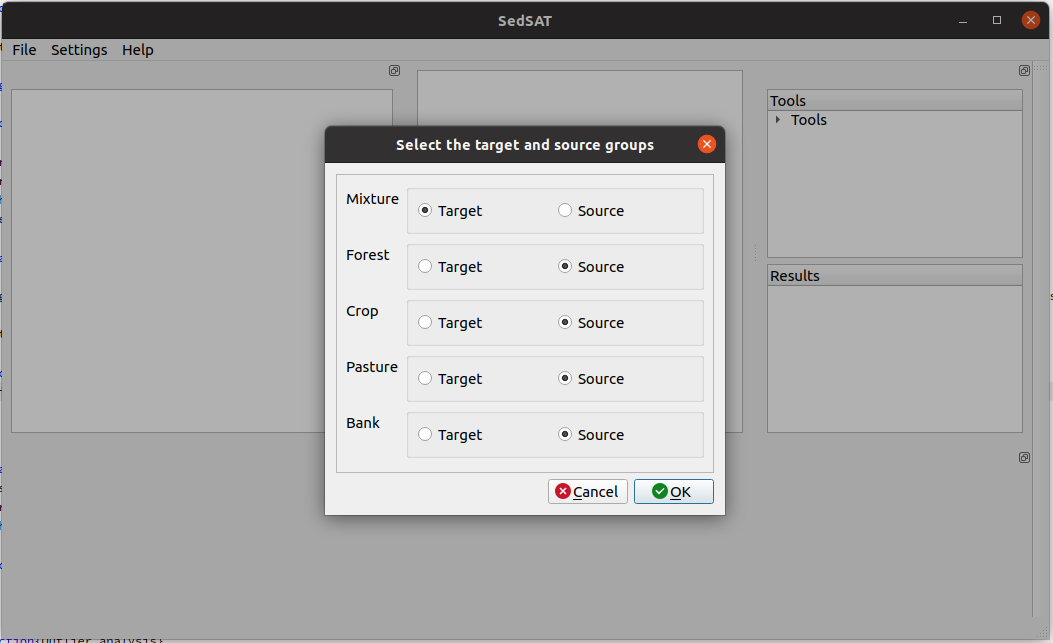
\includegraphics[width=\textwidth]{Figures/SelectSourceTargetGroups.png}
    \caption{Indicating the target sample}
    \label{fig:indicate_target_sample}
\end{figure}

After you identify the target sample sheet, SedSAT3 imports the data and opens the constituent properties table in the middle of the window (Fig.~\ref{fig:element_properties}). Samples are included or excluded separately, in \textbf{Settings}$\rightarrow$\textbf{Include/Exclude Samples} (Section~\ref{sec:choosing-samples}). Each window panel and individual columns can be resized by hovering your mouse between column headers; a double arrow will appear that lets you resize them for better viewing.

The middle window panel contains five columns. The constituents are listed in the first column. In the second column (Constituent Type), you can double-click on each entry to open a drop-down menu with the following options:

\begin{itemize}
    \item Element
    \item Isotope
    \item Particle size
    \item Organic carbon
    \item Exclude
\end{itemize}

To exclude a constituent from the analysis, click its box in the fifth column, \textit{Include in analysis}, so that it reads \textit{No}; click again to include it. The \textit{Include all elements} box above the table includes or excludes every constituent at once.

For isotopes, you must choose the base element and the standard isotope ratio. These are needed for converting $\delta$ values to the content of the isotope (Section~\ref{sec:stable-isotopes}). The \textit{Base Element} and \textit{Standard isotope ratio} cells can only be edited after the constituent's type has been set to \textit{Isotope}: set the type first. The base element must be measured in every sample. It is either an element included in the analysis, or the organic matter constituent; if an element used as a base is excluded, the fingerprinting tools stop with a message. In the example data:
\begin{itemize}
    \item for $\delta^{15}$N, the base element is N and the standard isotope ratio is $(^{15}\mathrm{N}/^{14}\mathrm{N})_\mathrm{air} = 0.003676$;
    \item for $\delta^{13}$C, the base element is TOC, the only carbon content measured, and the standard isotope ratio is $(^{13}\mathrm{C}/^{12}\mathrm{C})_\mathrm{VPDB} = 0.011180$.
\end{itemize}
TOC is also the organic matter constituent. As a base element it is not used as a tracer: it is not fitted, and the tools that test or select tracers leave it out. The fingerprinting tools only use it to weight the $\delta^{13}$C of each source by the source's organic carbon content, with the measured (uncorrected) TOC values. The value of the standard ratio does not affect the results, because it cancels in the $\delta$ value of the mixture (Eq.~\ref{eq:delta_mixture}).

Constituents designated as particle size or organic matter are not tracers: they are used only for the size and organic matter correction (Section~\ref{sec:sizeandorganiccorrection}). The tools that test or select tracers (analysis of variance, discriminant function analysis, discriminant power, auto-select and the bracketing test) never include them. In the example data, set D50 to \textit{Particle size} and TOC to \textit{Organic carbon} before running any analysis.

Constituents are listed alphabetically, in this table and in the results, rather than in the order of the Excel columns.

You can revisit the constituent properties at any time through the top menu item \textbf{Settings}$\rightarrow$\textbf{Constituent properties}.

\begin{figure}[ht]
    \centering
    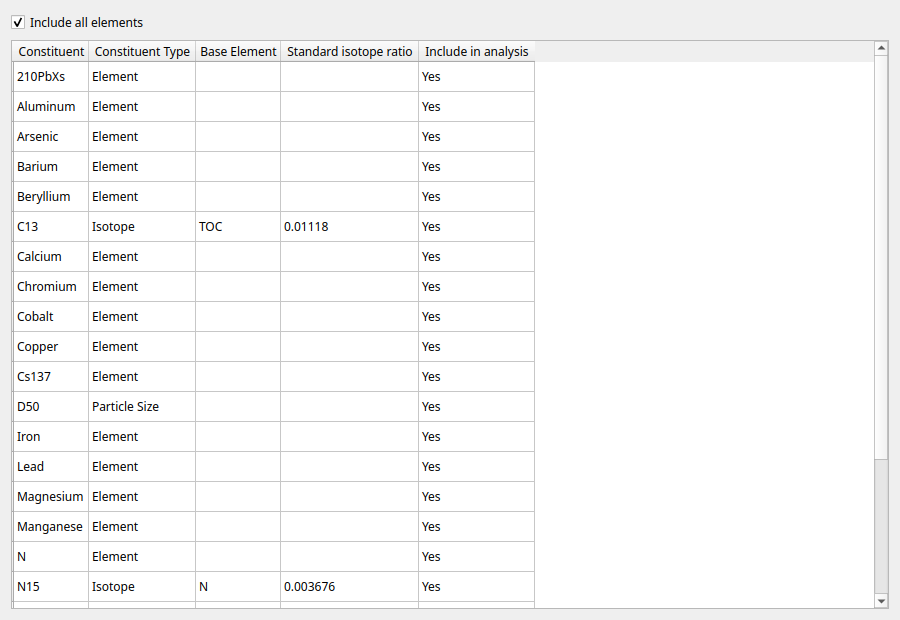
\includegraphics[width=\textwidth]{Figures/Element_Properties.png}
    \caption{Specifying constituents' properties}
    \label{fig:element_properties}
\end{figure}

Now is a good time to save your project using \textbf{File}$\rightarrow$\textbf{Save} or pressing \textbf{Ctrl+S}. The file is saved in a readable JSON format with the extension \texttt{.cmb} (CMB Source file). You can open it in any text editor to inspect its contents, and you can reload the project at any time.

You can visualize the elemental profiles using the tree view on the left side of the screen labeled \textbf{Data}: select any element to display its values in every group (Fig.~\ref{fig:constituents_vis}). The vertical axis is logarithmic, except for a constituent with zero or negative values (such as $\delta^{13}$C), which is shown on a linear axis.

\begin{figure}[ht]
    \centering
    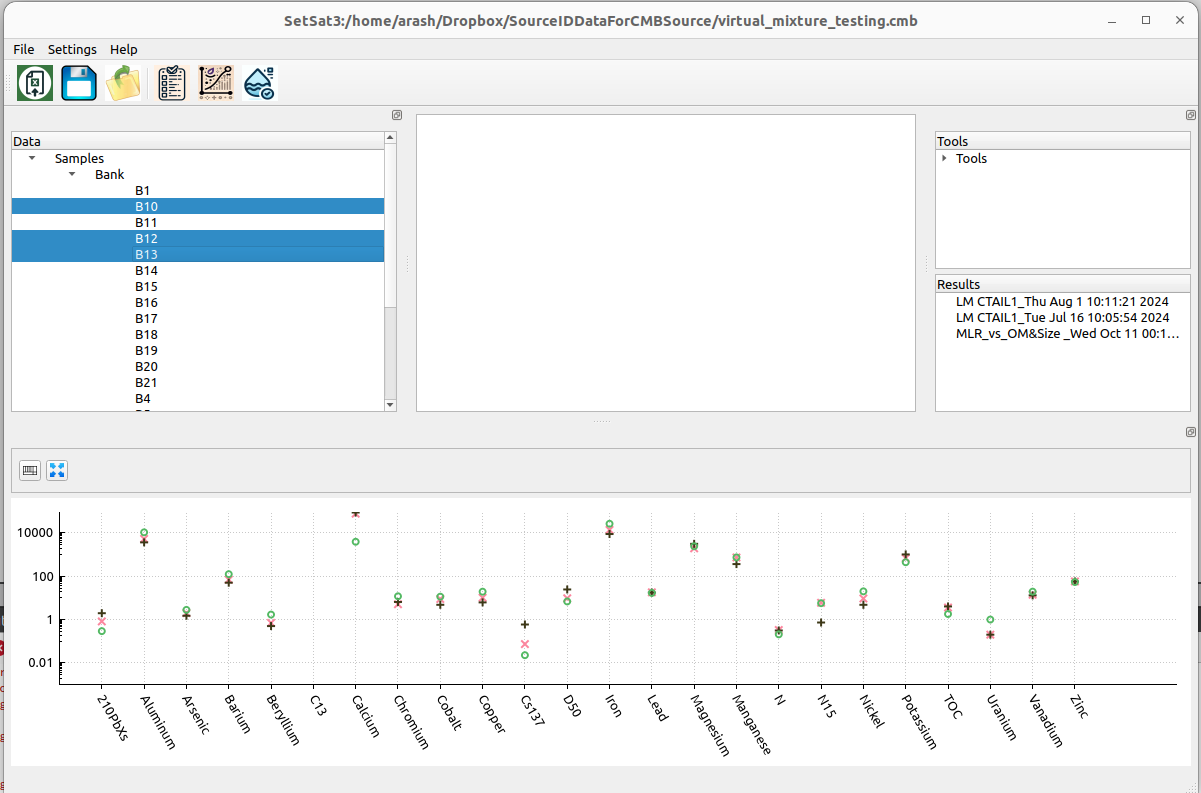
\includegraphics[width=\textwidth]{Figures/Constituent_Viz.png}
    \caption{Visualizing the raw data}
    \label{fig:constituents_vis}
\end{figure}

\subsubsection{Choosing samples to be discarded}\label{sec:choosing-samples}
To include or exclude samples, choose \textbf{Settings}$\rightarrow$\textbf{Include/Exclude Samples} from the menu. This dialog lets you mark individual samples for exclusion from all subsequent analyses without removing them from the dataset. To exclude a sample, click the \textbf{Include} cell next to its name so that it reads \texttt{No}; click again to include it.

Choose the group to show from the drop-down list at the top of the dialog; there is one entry per source group and one for the target samples. The table shows three columns:

\begin{itemize}
    \item \textbf{Sample} --- the sample name as imported from Excel.
    \item \textbf{Include} --- whether the sample is included in the analysis. Click a cell to toggle between \texttt{Yes} and \texttt{No}.
    \item \textbf{Notes} --- automatically populated annotations, such as which elements (if any) were flagged as outliers. Samples with outlier flags are shown in red (see Section~\ref{sec:outlier_analysis}). Flagged samples are not excluded automatically: you decide, and exclude a sample by setting its \textbf{Include} cell to \texttt{No}.
\end{itemize}

Each time the dialog is opened, SedSAT3 runs the outlier test on every source group (Section~\ref{sec:outlier}), after asking for the threshold, and fills the \textbf{Notes} column. A sample is flagged only if one of its values lies beyond the threshold; with the example data and the default threshold of 3, no sample is flagged. You can leave all samples included for now and revisit this dialog later, after running the outlier analysis, organic matter and particle size regressions, or any other diagnostic that may suggest a sample should be discarded.

To exclude a sample at any time, return to this dialog through \textbf{Settings}$\rightarrow$\textbf{Include/Exclude Samples} in the top menu, then click the \textbf{Include} cell next to the sample name so that it reads \texttt{No}. Excluded samples remain in the project file but are skipped by all analyses that respect the include/exclude flag. To re-include a sample later, set the value back to \texttt{Yes}.

\begin{tcolorbox}[colback=yellow!10,colframe=yellow!50!black,title=Note]
Do not deselect target samples at this stage. Target samples are listed under the target group in the drop-down list, but the include/exclude flag for target samples is used only by certain batch tools. For deterministic and Bayesian fingerprinting, the target sample is selected explicitly when each analysis is run.
\end{tcolorbox}
\chapter{Deterministic Fingerprinting Tools}\label{chap:deterministic}
This chapter outlines the complete sequence of steps and tools required to perform maximum-likelihood (deterministic) sediment fingerprinting. The process consists of the following steps, in order: outlier analysis (Section~\ref{sec:outlier}), organic matter and particle size correction (Section~\ref{sec:sizeandorganiccorrection}), and bracketing analysis (Section~\ref{sec:bracketing}). Section~\ref{sec:dfa-theory} introduces the theoretical basis of discriminant function analysis (DFA), which is then applied in Section~\ref{sec:multiway-dfa} to perform multi-way stepwise DFA across all source groups --- the standard tracer-selection step in the workflow. The chapter concludes with the fingerprinting procedure itself, available as a single-sample tool (Section~\ref{sec:lmmle}) and a batch tool (Section~\ref{sec:fingerprinting-batch}).

\section{Outlier analysis}
\label{sec:outlier_analysis}\label{sec:outlier}
The outlier analysis detects possible outliers in the elemental content of individual samples. For each source group, it first maps the concentration of each element using the Box--Cox transformation to bring its distribution as close as possible to a Gaussian:
\begin{equation}
     \hat{y}_{i,j,k} = \begin{cases}
   \dfrac{\left(\dfrac{y_{i,j,k}}{\sigma_{i,j}}\right)^{\lambda}-1}{\lambda} & \text{for } \lambda \neq 0 \\[1.5em]
   \log\left(\dfrac{y_{i,j,k}}{\sigma_{i,j}}\right) & \text{for } \lambda = 0
\end{cases}
\end{equation}
where $\sigma_{i,j}$ is the standard deviation of element $j$ in source group $i$.

The outlier analysis module first finds the optimal value of $\lambda$ that brings the transformed elemental concentrations closest to a normal distribution, then transforms the data using this optimal $\lambda$. Normality is assessed using the Kolmogorov--Smirnov test. The Box--Cox transformation needs positive values: a constituent with a zero or negative value (for example $\delta^{13}$C) is not transformed, and its $\lambda$ is reported as 1. To view the optimal values of $\lambda$, use \textbf{Tools}$\rightarrow$\textbf{Other Statistical Tools}$\rightarrow$\textbf{Data exploration}$\rightarrow$\textbf{Optimal Box-Cox parameters}.

After the Box--Cox transformation, the outlier analysis feature reports the deviation from the mean for each element in each sample of the selected source group. The deviation measure is calculated as:
\begin{equation}
    z = \frac{y_i - \mu}{\sigma}
\end{equation}
where $\mu$ and $\sigma$ are the mean and standard deviation of the transformed elemental content in the group.

\textbf{SedSAT3 runs the outlier test on every source group each time you open Settings$\rightarrow$Include/Exclude Samples.} A dialog first asks for the threshold (3 by default). A window like Fig.~\ref{fig:include_exclude_samples} then appears. Samples that contain an element flagged as an outlier are shown in red, and the \textbf{Notes} column names the elements. Outliers are shown one source group at a time; choose the group from the drop-down list at the top. Outliers are not removed automatically: to exclude a sample from further analysis, click the \textbf{Include} cell next to the sample name so that it reads \texttt{No}. Although target samples are listed, they should not be deselected.

\begin{figure}[ht]
    \centering
    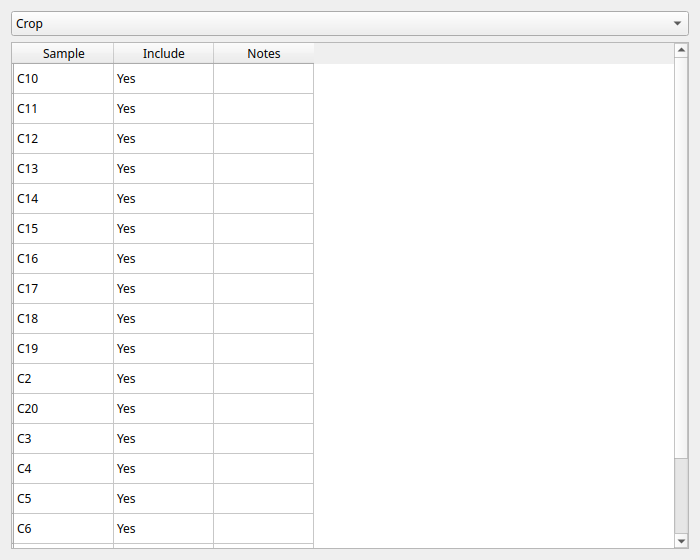
\includegraphics[width=\textwidth]{Figures/Include_Exclude_samples.png}
    \caption{Including or excluding samples from the analysis}
    \label{fig:include_exclude_samples}
\end{figure}
\FloatBarrier

To see the deviations themselves, double-click \textbf{Tools}$\rightarrow$\textbf{Deterministic Sediment Fingerprinting}$\rightarrow$\textbf{1-Outlier Analysis}. This tool reports the deviations for one source group at a time: select the group in the form. (The test in the Include/Exclude Samples dialog covers every group.) The threshold sets the value of $|z|$ above which an item is highlighted in red.

Click the \textbf{Ok} button at the bottom of the form, then click the table button~
\includegraphics[width=0.5cm]{Figures/table.png} on the window that appears. A table like Figure~\ref{fig:outlier_table} will be displayed. Values outside the specified threshold are highlighted in red.

If you want to remove a sample based on the outlier analysis, go to \textbf{Settings}$\rightarrow$\textbf{Include/Exclude Samples} in the top menu, then click the sample's \textbf{Include} cell. The entry will change to `No' (Fig.~\ref{fig:include_exclude_samples}).

\begin{figure}[ht]
    \centering
    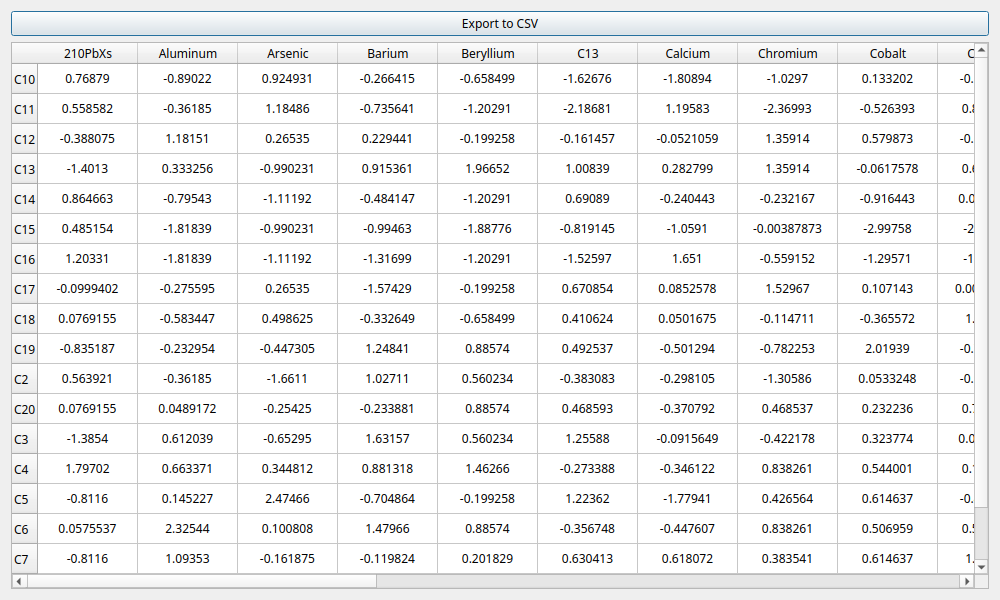
\includegraphics[width=\textwidth]{Figures/Outlier_table.png}
    \caption{Outlier table}
    \label{fig:outlier_table}
\end{figure}

\FloatBarrier

\section{Organic matter and particle size correction}\label{sec:sizeandorganiccorrection}
In sediment source fingerprinting, organic matter and particle size corrections are important when identifying and apportioning sediment sources within a watershed or catchment. These corrections account for variation in organic matter content and grain size distribution among different sediment sources, such as soil erosion, agricultural activities, and construction (Gorman-Sanisaca et al., 2017). Specifically, they account for the fact that the fraction of particles mobilized from a source may have a different organic matter content and size distribution than the bulk samples collected to represent that source. To make these corrections, SedSAT3 fits a multiple linear or non-linear regression relating the elemental content of each element to organic matter content and the mean or effective particle size. The fitted relationship is then used to correct each source sample's elemental content using the organic matter content and particle size of the target sample.

SedSAT3 provides two regression options: linear regression and power-law regression.

Linear regression:
\begin{equation}
    y = a + \sum_i b_i e_i
\end{equation}

Power regression:
\begin{equation}
    \ln(y) = a + \sum_i b_i \ln(e_i)
\end{equation}

where $a$ is the intercept, $b_i$ is the coefficient for independent variable $i$, and $e_i$ is the value of independent variable $i$. The independent variables can be particle size, organic matter content, or both. Once the regression coefficients and intercept have been estimated, the corrected value of each element in each source sample is computed as follows.

Linear regression:
\begin{equation}
    y_c = y + \sum_i b_i (e_{i,t} - e_{i,s})
\end{equation}

Power regression:
\begin{equation}
    y_c = y \prod_i \left(\frac{e_{i,t}}{e_{i,s}}\right)^{b_i}
\end{equation}

where $e_{i,t}$ is the value of independent variable $i$ in the target sample, and $e_{i,s}$ is the value of independent variable $i$ in the source sample.

When both organic matter and particle size are used, they are the two independent variables of a single multiple regression, fitted to the raw data of each source group, and the correction applies both terms at once. The particle size correction is not applied first, with the organic matter correction then fitted to the size-corrected data. Only the terms you select for correction (by default, those with a p-value below the threshold, except for isotopes, which are not corrected by default) are applied. The regressions are fitted separately for each element and each source group; the same coefficients are used for every sample of a group, each corrected with its own organic matter content and particle size. Because the correction moves each source sample towards the organic matter content and particle size of one target sample, the corrected data, and every result computed from them, depend on the target sample chosen.

\begin{tcolorbox}[colback=yellow!10,colframe=yellow!50!black,title=Note]
A linear correction can over-correct: when the target sample's organic matter content or particle size is far from a source sample's, $y_c$ can become zero or negative, which is outside the physical range of a concentration. SedSAT3 then stops the analysis with a message naming the element and group (``after the organic matter and size correction; the imported values are positive''). The power regression cannot produce negative values. If this happens, use the power regression, or do not apply the correction to the elements named.
\end{tcolorbox}

\subsubsection{Performing organic matter and particle size correction}

In the tools window, click \textbf{Tools}$\rightarrow$\textbf{Deterministic Sediment Fingerprinting}$\rightarrow$\textbf{2-Organic matter and particle size correction}.

In the form that appears, select the regression equation, \textit{Linear} or \textit{Power}, from the \textbf{Equation} drop-down menu, then select the constituents representing organic matter and particle size. If a constituent representing organic matter or particle size is not available, or if you only want to correct based on one of them, leave the unused field blank. Click \textbf{Ok} at the bottom of the form. One run fits the regressions for every source group. The results window that appears contains one panel per group, with the regression results for every constituent. To visualize the regressions, click the graph button~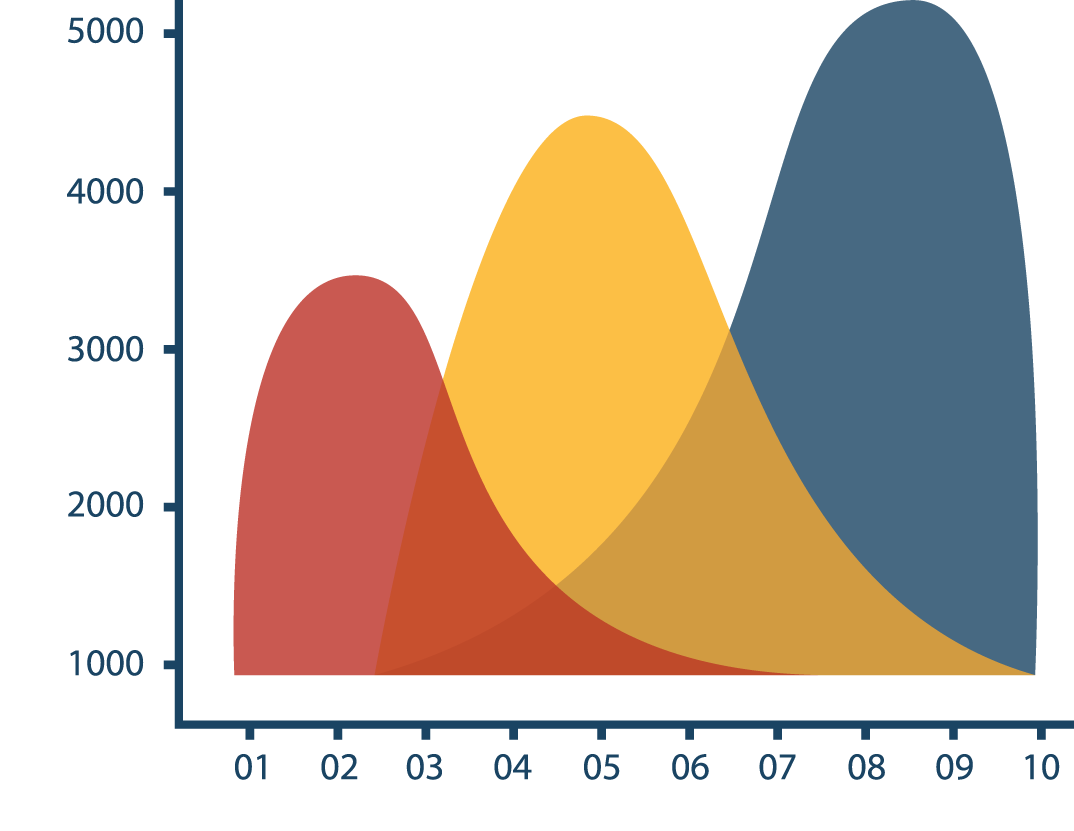
\includegraphics[width=0.5cm]{Figures/Graph.png}. A window like Fig.~\ref{fig:regression_results} will appear: the points are the measured (uncorrected) values and the line is the fitted regression. Use the combo boxes at the top to select different constituents and independent variables. The corrected values are shown by the tool described in Section~\ref{sec:view-corrected}.

\begin{figure}[ht]
    \centering
    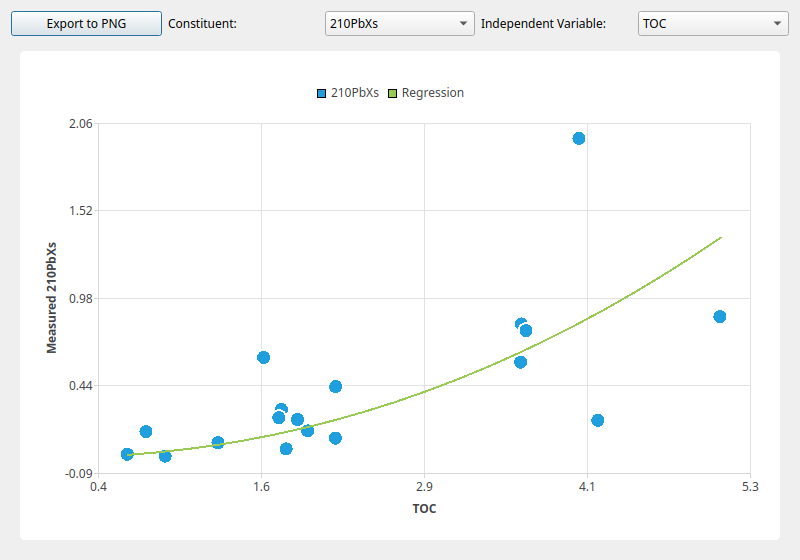
\includegraphics[width=\textwidth]{Figures/Regression_results.png}
    \caption{Graphical representation of OM and size correction regressions}
    \label{fig:regression_results}
\end{figure}
\FloatBarrier

To see the regression results in tabular form, click the table button~
\includegraphics[width=0.5cm]{Figures/table.png} on the side of each source group in the results window.

\begin{figure}[ht]
    \centering
    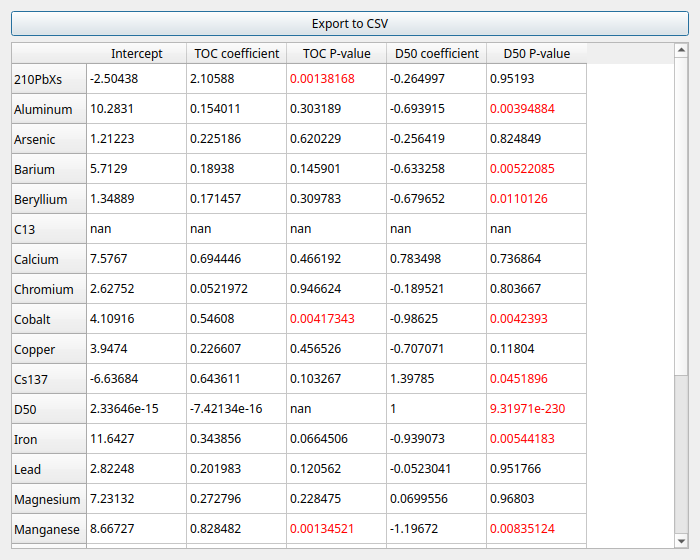
\includegraphics[width=\textwidth]{Figures/Regression_Tabular_results.png}
    \caption{OM and size correction results}
    \label{fig:regression_table}
\end{figure}
\FloatBarrier

The table reports the p-values indicating the statistical significance of organic matter and size as predictors. Values below the selected threshold (e.g., 0.05) are shown in red. (A constituent regressed on itself, such as D50 in its own row, has no meaning and is never corrected.)

\subsubsection{Viewing the corrected elemental profiles}\label{sec:view-corrected}
Based on the p-values for the OM and size coefficients, you can decide whether to apply each correction. From the top menu, select \textbf{Settings}$\rightarrow$\textbf{Organic Matter and Size Correction}. A form containing the regression results will appear in the middle panel (Fig.~\ref{fig:indicate_om_and_size_correction}).

\begin{figure}[ht]
    \centering
    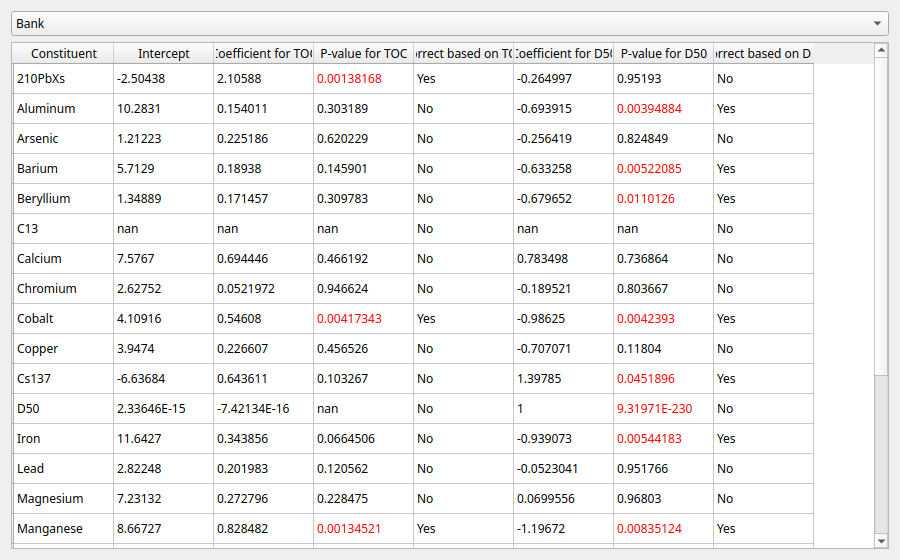
\includegraphics[width=\textwidth]{Figures/IndicateOMandSizeCorrection.png}
    \caption{Indicating OM and size correction}
    \label{fig:indicate_om_and_size_correction}
\end{figure}
\FloatBarrier

The combo box at the top lets you navigate between source groups. The columns \textbf{P-value for TOC} and \textbf{P-value for D50} display the p-values for the regression coefficients on organic matter and particle size, respectively. The columns \textbf{Correct based on TOC} and \textbf{Correct based on D50} let you specify whether to apply each correction for each element. Elements with a p-value below 0.05 are selected for correction by default. Isotopes are not selected, whatever their p-values: $\delta$ values depend on the relative proportions of organic matter, so correcting them would bias them \citep{gormansanisaca2017determining}. You can still select them here.

To view how the correction affects the elemental profiles of the source groups for a specific target sample, choose \textbf{Tools}$\rightarrow$\textbf{Other Statistical Tools}$\rightarrow$\textbf{Data exploration}$\rightarrow$\textbf{Correct based on size and organic matter} from the tools panel. This tool does not fit anything: it applies the regressions of the last run of step~2 and shows the result. In the form in the middle panel, choose the target sample on which to base the correction. The results window will contain a panel for each source group. To see the corrected elemental profiles for any source group, click the table button~
\includegraphics[width=0.5cm]{Figures/table.png} on the side of that panel (Fig.~\ref{fig:corrected_elements_table}), or the graph button to plot them.

\begin{figure}[ht]
    \centering
    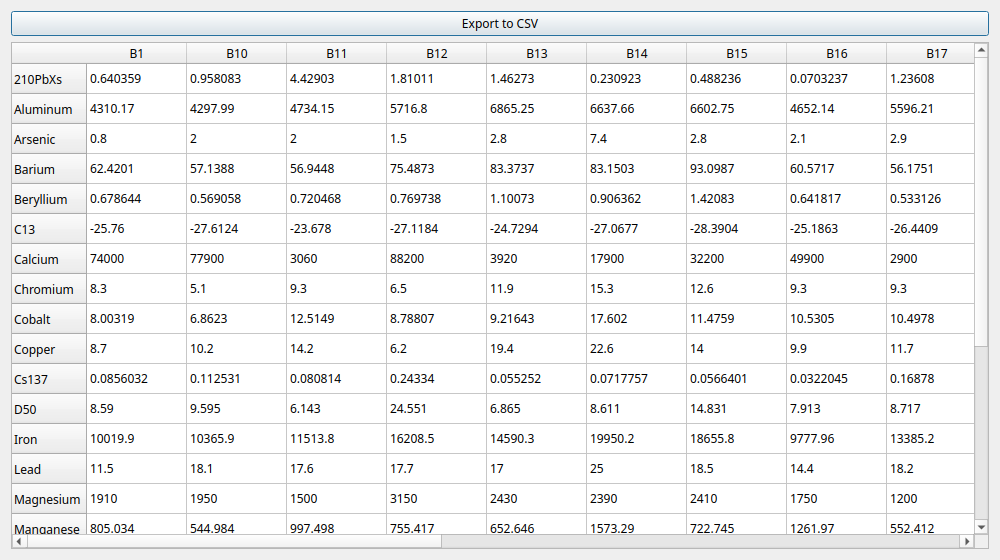
\includegraphics[width=\textwidth]{Figures/CorrectedEPsTable.png}
    \caption{Corrected elemental profiles based on size and organic matter}
    \label{fig:corrected_elements_table}
\end{figure}
\FloatBarrier

You can export the corrected elemental profiles to a CSV file to compare them with the original values, which are shown by \textbf{Data} in the tree view on the left.

\section{Bracketing analysis}\label{sec:bracketing}

A bracketing analysis checks whether any element in the target sample has a value higher than in all the source samples, or lower than in all of them. If the content of a particular element in the target sample lies outside the range of every source sample, no linear combination of sources can reproduce an elemental profile close to the target's, and that element should be excluded from the analysis.

To perform a bracketing analysis, go to \textbf{Tools}$\rightarrow$\textbf{Deterministic Sediment Fingerprinting}$\rightarrow$\textbf{3-Bracketing Analysis} in the tools window. Choose whether to run the bracket test on samples corrected for size and organic matter, and whether to use only selected samples and elements, then click \textbf{Ok}. The test is run for every target sample at once; with the correction, each target sample is tested against the sources corrected for that sample. The results window contains a table with one row per constituent and one column per target sample, marking each test as passed or failed. To view the results in tabular form or export them to a CSV file, click the table button~
\includegraphics[width=0.5cm]{Figures/table.png} (Fig.~\ref{fig:bracketing_results}).

Elements that fail the bracket test must be removed manually: go to \textbf{Settings}$\rightarrow$\textbf{Constituent Properties}, then in the \textbf{Include in analysis} column, click each element that did not pass the bracket test so that it reads \textit{No}. The bracket results can be exported (table button, \textbf{Export to CSV}) as a record of why each element was excluded. Once all failing elements have been excluded, you can proceed to the next step in sediment fingerprinting: \textbf{4-Stepwise Discriminant Function Analysis}.

\begin{tcolorbox}[colback=yellow!10,colframe=yellow!50!black,title=Note]
Bracketing results are specific to each target sample: an element can fail for one target sample and pass for another. The constituent selection, however, is one list for the whole project. When you fingerprint one target sample, exclude the elements that fail for that sample. When you move on to another target sample, include all elements again in \textbf{Settings}$\rightarrow$\textbf{Constituent Properties} and exclude those that fail for the new sample, using its column of the same table. For the batch tools, which use one selection for every target sample, exclude every element that fails for any target sample (Section~\ref{sec:fingerprinting-batch}).
\end{tcolorbox}

\begin{figure}[ht]
    \centering
    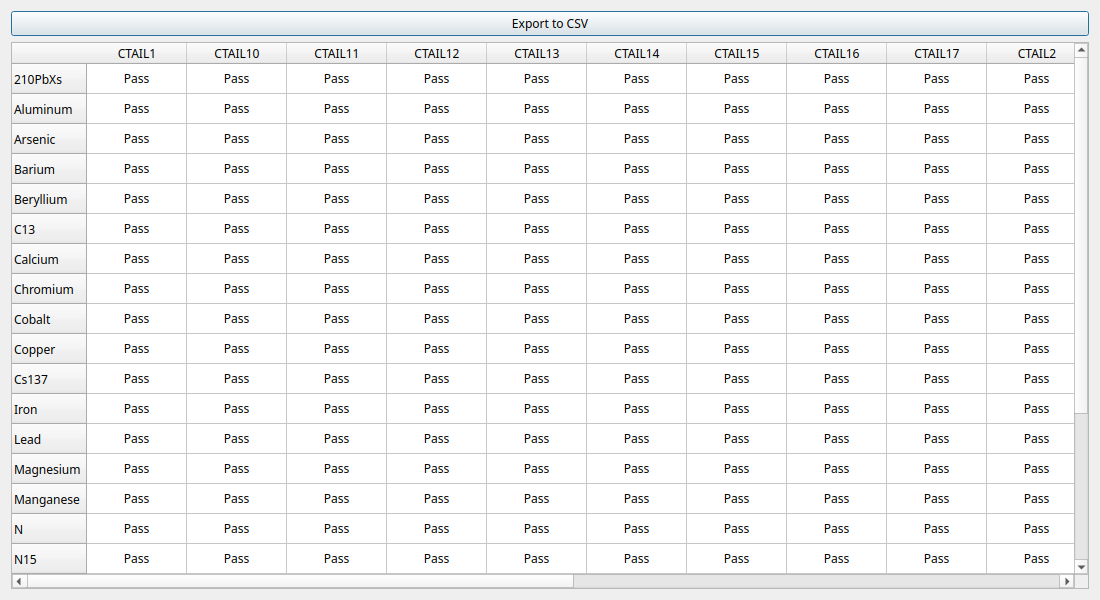
\includegraphics[width=\textwidth]{Figures/Bracketing.png}
    \caption{Bracketing test results}
    \label{fig:bracketing_results}
\end{figure}
\FloatBarrier

\section{Stepwise Discriminant Function Analysis (DFA)}\label{sec:dfa-theory}
Once the bracketing analysis has identified the elements suitable for inclusion, the next step is to select from among those a subset that best discriminates between source groups. This section introduces the theoretical basis of discriminant function analysis (DFA); Section~\ref{sec:multiway-dfa} describes how SedSAT3 applies it across all source groups simultaneously.

Discriminant function analysis is a multivariate statistical technique used to predict the group membership of individuals or objects based on a set of predictor variables, by finding a linear combination of those variables that maximally discriminates between two or more groups \citep{collins2010tracing}. The method determines a discriminant function that separates observations from different groups by reducing within-group variability while increasing between-group variability. In the context of sediment fingerprinting, DFA is used to identify which elements most effectively differentiate between two or more sources. The linear discriminant function provides a scalar value calculated as a linear combination of the elemental contents for each sample:
\begin{equation}\label{eq:discriminant_score}
    D(\tilde{\mathbf{y}}_k) = \mathbf{w}^T \tilde{\mathbf{y}}_k + c
\end{equation}
where $D(\tilde{\mathbf{y}}_k)$ is the discriminant score of sample $k$, $\mathbf{w}$ is a vector of weights, $\tilde{\mathbf{y}}_k$ is the vector containing the elemental profile of sample $k$, and $c$ is a constant.

SedSAT3 uses Fisher's linear discriminant method \citep{fisher1936use}. The discriminant functions are found by solving an optimization problem that maximizes the Fisher criterion, which is the ratio of between-class variance to within-class variance:
\begin{equation}
    J(\mathbf{w}) = \frac{\mathbf{w}^T S_b \mathbf{w}}{\mathbf{w}^T S_w \mathbf{w}}
\end{equation}
where $S_b$ is the between-class scatter matrix, which measures the variance between group means, and $S_w$ is the within-class scatter matrix, which measures the variance within groups.

This criterion is maximized by finding the eigenvectors of the matrix $S_w^{-1} S_b$. The eigenvectors corresponding to the largest eigenvalues are the directions (weights) that define the discriminant functions:
\begin{equation}
    S_w^{-1} S_b \mathbf{w} = \lambda \mathbf{w}
\end{equation}
The weight vector is obtained as the eigenvector corresponding to the eigenvalue with the largest absolute value. Its components are the weights $\mathbf{w}$ of Eq.~\eqref{eq:discriminant_score}: the discriminant score of a sample is the weighted sum of its constituent values, and the constituents with the largest weights (in absolute value, relative to their spread) contribute most to the separation. SedSAT3 shows the weight vectors in the \textit{Eigen vector} panel of the discriminant function analysis tools.

Fisher's method assumes that the constituents are approximately multivariate normal within each group, with similar covariance matrices. SedSAT3 does not test multivariate normality. The \textit{Box-cox transformation} option of the DFA tools transforms each constituent towards normality before the analysis, which improves the marginal normality; the Kolmogorov--Smirnov tools (Section~\ref{sec:ks-individual}) can be used to check individual constituents.

Wilks' Lambda, $\Lambda$, measures the ratio of within-group variability to total variability:
\begin{equation}
    \Lambda = \frac{|S_w|}{|S_b + S_w|}
\end{equation}

The associated $\chi^2$ statistic is calculated as:
\begin{equation}
    \chi^2 = -\left(n - 1 - \frac{p + g}{2}\right) \ln(\Lambda)
\end{equation}
with $df = p \times (g - 1)$ degrees of freedom, where $n$ is the total number of samples across all source groups, $p$ is the total number of elements, and $g$ is the number of groups.

An F-test can also be used to test the null hypothesis that the centroids of the discriminant scores (Eq.~\ref{eq:discriminant_score}) are the same for all groups.

\paragraph{Stepwise selection.} With many constituents and few samples, a DFA on all constituents at once is poorly conditioned: tracers in sediment fingerprinting data are often strongly correlated, because they respond together to particle size, organic content and geochemistry, and the analysis can overfit when the number of constituents approaches the number of samples. The stepwise tools therefore use forward selection: they start with the constituent that best separates the groups and add one constituent at a time, each time the one that most improves the separation, reporting the statistics after each addition. A constituent that adds little once others are in is not selected, which removes redundant, correlated tracers. The constituents up to the smallest $\chi^2$ p-value are selected.

\section{Multi-way stepwise discriminant function analysis}\label{sec:multiway-dfa}

Step~4 performs forward stepwise discriminant function analysis among all source groups at once (multi-way): the separation measured is that of every source group from all the other source samples taken together. It selects the constituents that best discriminate between the source groups.

To run it, choose \textbf{Tools}$\rightarrow$\textbf{Deterministic Sediment Fingerprinting}$\rightarrow$\textbf{4-Stepwise discriminant function analysis (Multi-way)}. In the form:
\begin{itemize}
    \item \textit{Box-cox transformation}: run the analysis on Box--Cox transformed data.
    \item \textit{OM and Size Correct based on target sample}: run it on data corrected for the target sample chosen (leave blank for uncorrected data). Because the correction depends on the target sample, the selection can differ between target samples; see the note below.
    \item \textit{Modify the included elements based on the results}: when checked, the constituents that are not selected are excluded in \textbf{Settings}$\rightarrow$\textbf{Constituent Properties}, so that fingerprinting (steps 5 and 6) uses only the selected ones. They stay excluded for every later tool until you include them again (see the note in Section~\ref{sec:shared-settings}). Leave it unchecked to look at the results first.
    \item \textit{Use only selected elements} and \textit{Use only selected samples}: Section~\ref{sec:shared-settings}.
\end{itemize}
Click \textbf{Ok}.

The result window contains seven panels:
\begin{enumerate}
    \item \textit{Chi-squared P-Values}: the $\chi^2$ p-value after each constituent is added, in the order added (Fig.~\ref{fig:Chi2-DFA-multiway}). The first constituent is the one that best separates the groups on its own; each later one is the constituent that most improves the separation of those already in. A smaller p-value means a stronger separation.
    \item \textit{Elements to be Selected}: the constituents up to the smallest p-value, which are the ones selected.
    \item \textit{Wilks' Lambda} after each addition (Fig.~\ref{fig:Wilks-DFA-multiway}). It always decreases as constituents are added, so the selection is based on the p-value, which accounts for the number of constituents.
    \item \textit{F-test P-Value} after each addition.
    \item \textit{Multiway Projected Elemental Profiles (selected constituents)}: the discriminant scores of the source samples, computed with the selected constituents (Fig.~\ref{fig:Multiway-DFA-scatter-plots}).
    \item \textit{Eigen vectors (selected constituents)}: the weights of the selected constituents in each source group's discriminant function (Fig.~\ref{fig:Multiway-eigenvectors}).
    \item \textit{Confusion matrix (selected constituents, leave-one-out)}: how well the selected constituents classify the source samples (Fig.~\ref{fig:confusion-matrix}).
\end{enumerate}
All four of the first panels list the constituents in the same order, the order in which they were added. The p-values are given per constituent added; to see the statistics per source group, run \textbf{Discriminant function analysis (Multi-way)} on the selected constituents (Section~\ref{sec:dfa-tools}).

In the example (Fig.~\ref{fig:Chi2-DFA-multiway}), C13 is added first, then Cs137, Potassium, Calcium, Iron, N and 210PbXs; the p-value is smallest after 210PbXs, so these seven constituents are selected. The p-values are very small (below $10^{-12}$), so the chart shows their base-10 logarithm.

\begin{tcolorbox}[colback=yellow!10,colframe=yellow!50!black,title=Note]
Only the elements marked for inclusion are used by the fingerprinting tools, all with the same weight: the DFA selects constituents, but its weights are not used in fingerprinting. When the analysis uses the organic matter and size correction, the selection is for the target sample chosen; for another target sample, run step~4 again with that sample.
\end{tcolorbox}

\begin{figure}[ht]
    \centering
    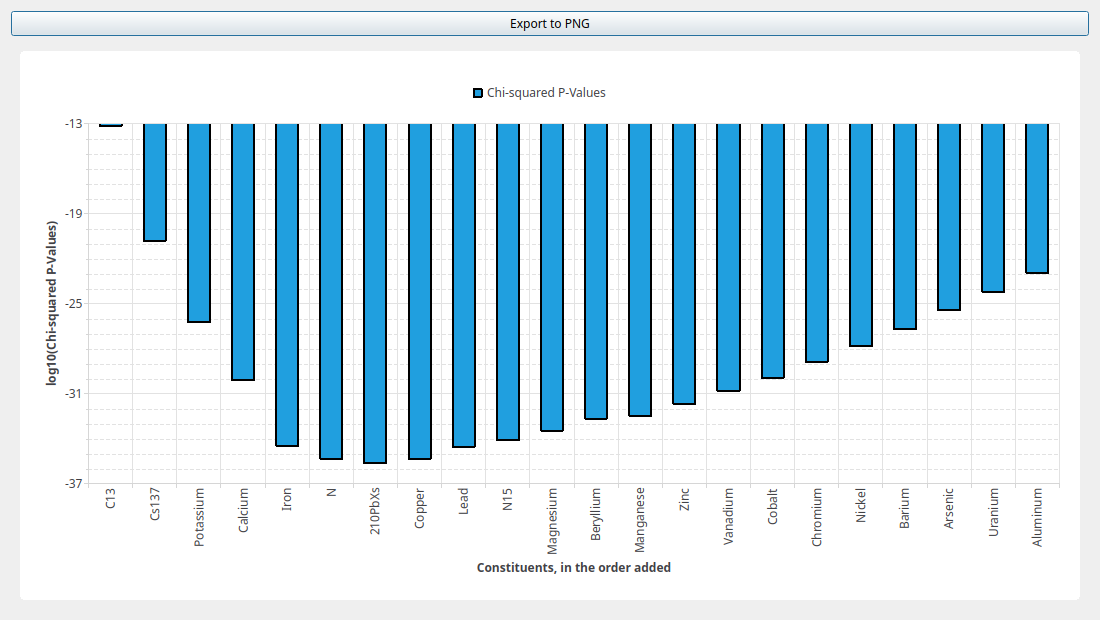
\includegraphics[width=\textwidth]{Figures/Chi2p-value-stepwise-multiway-DFA.png}
    \caption{Base-10 logarithm of the $\chi^2$ p-value after each constituent is added, in the order added, for multi-way stepwise DFA of the example data.}
    \label{fig:Chi2-DFA-multiway}
\end{figure}
\FloatBarrier

\begin{figure}[ht]
    \centering
    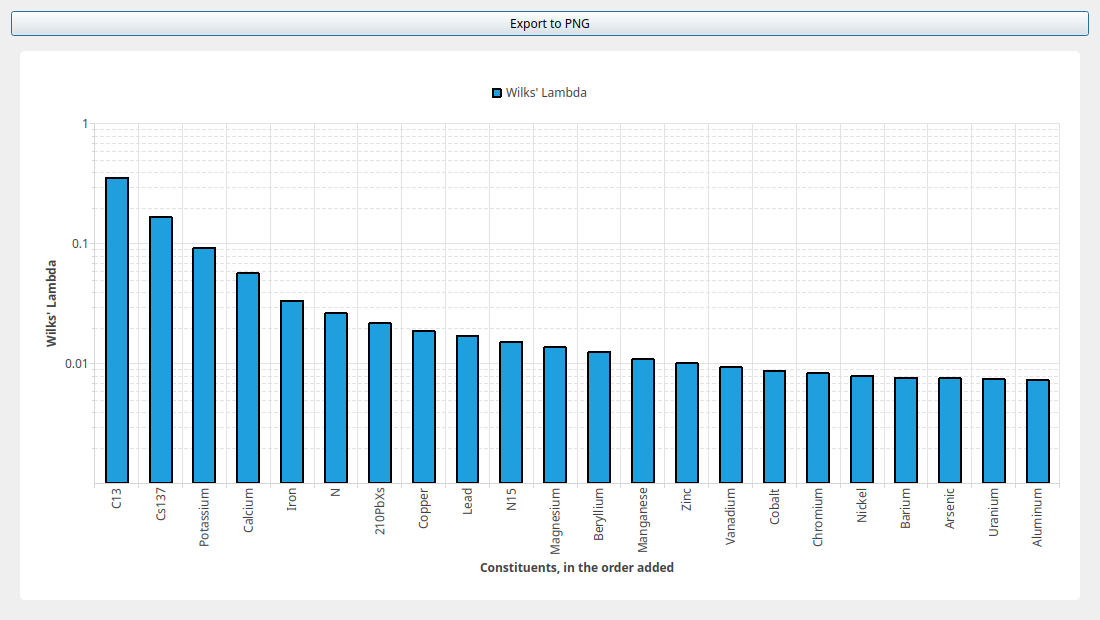
\includegraphics[width=\textwidth]{Figures/Wilks-Lambda-stepwise-multiway-DFA.png}
    \caption{Wilks' $\Lambda$ after each constituent is added, for multi-way stepwise DFA of the example data.}
    \label{fig:Wilks-DFA-multiway}
\end{figure}
\FloatBarrier

The statistics for each source group, computed with the selected constituents, are given by \textbf{Tools}$\rightarrow$\textbf{Other Statistical Tools}$\rightarrow$\textbf{Discriminant function analysis}$\rightarrow$\textbf{Discriminant function analysis (Multi-way)} with \textit{Use only selected elements} checked (Fig.~\ref{fig:Chi2-DFA-multiway-for-selected-elements}). A larger p-value for a group indicates weaker separation between that group and the rest.

\begin{figure}[ht]
    \centering
    \begin{tabular}{cc}
        a) & b) \\
        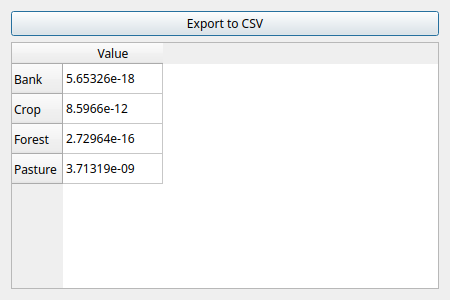
\includegraphics[width=0.46\textwidth]{Figures/DFA-Multiway-Chi2-p-value-table.png} &
        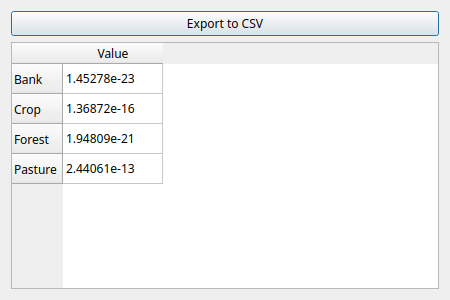
\includegraphics[width=0.46\textwidth]{Figures/DFA-Multiway-F-test-p-value-table.png}
    \end{tabular}
    \caption{a) $\chi^2$ p-values and b) F-test p-values between each source group and the rest of the samples, from \textbf{Discriminant function analysis (Multi-way)} on the seven constituents selected in step~4 (C13, Cs137, Potassium, Calcium, Iron, N and 210PbXs).}
    \label{fig:Chi2-DFA-multiway-for-selected-elements}
\end{figure}
\FloatBarrier

The fifth panel contains the discriminant scores of the source samples. Click the graph button~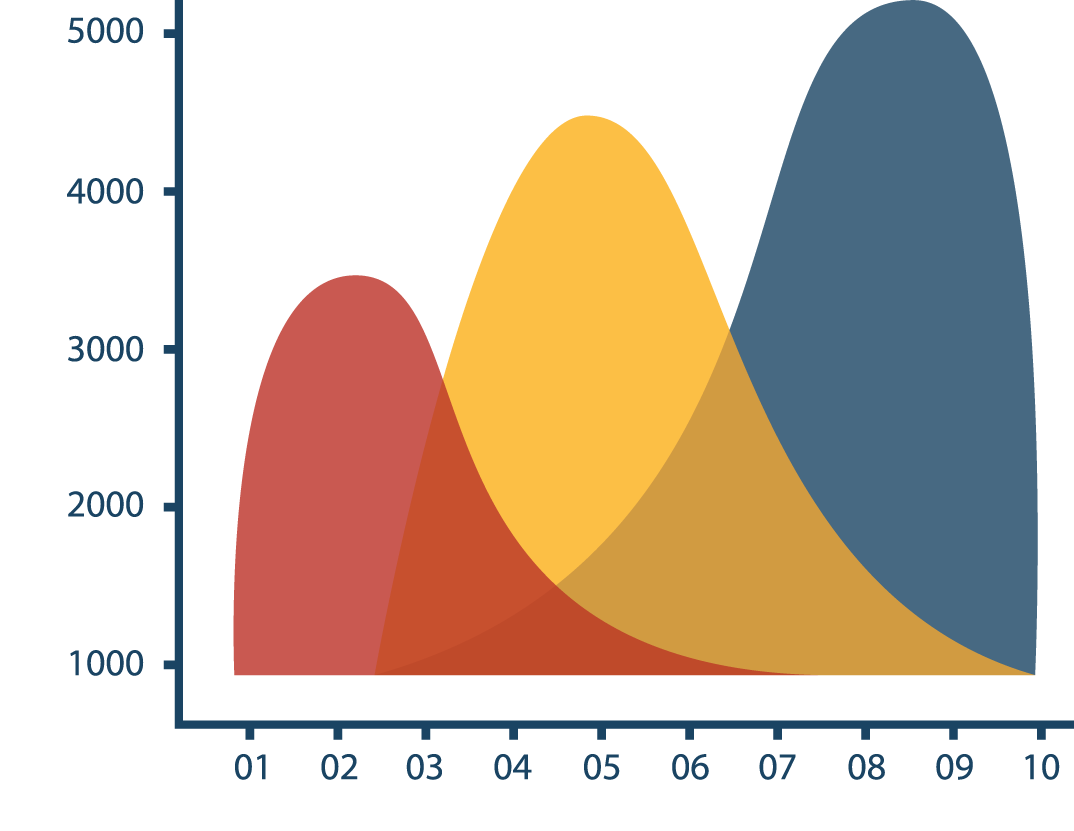
\includegraphics[width=0.5cm]{Figures/Graph.png} on the side of the panel. In the graph window that appears, use the drop-down menus at the top to choose two source groups (Fig.~\ref{fig:Multiway-DFA-scatter-plots}). The x-axis is each sample's score on the discriminant function that best separates the first group from the rest (``Discriminant score, Bank vs.\ the rest''); the y-axis is its score on the function of the second group. Every source group is plotted, each in its own color, which stays the same for every choice of groups; the dashed ellipses outline the spread of each group's samples (from their means, standard deviations and correlation). Groups whose clouds of points do not overlap are well separated by the selected constituents.

\begin{figure}[ht]
    \centering
    \begin{tabular}{cc}
        a) & b) \\
        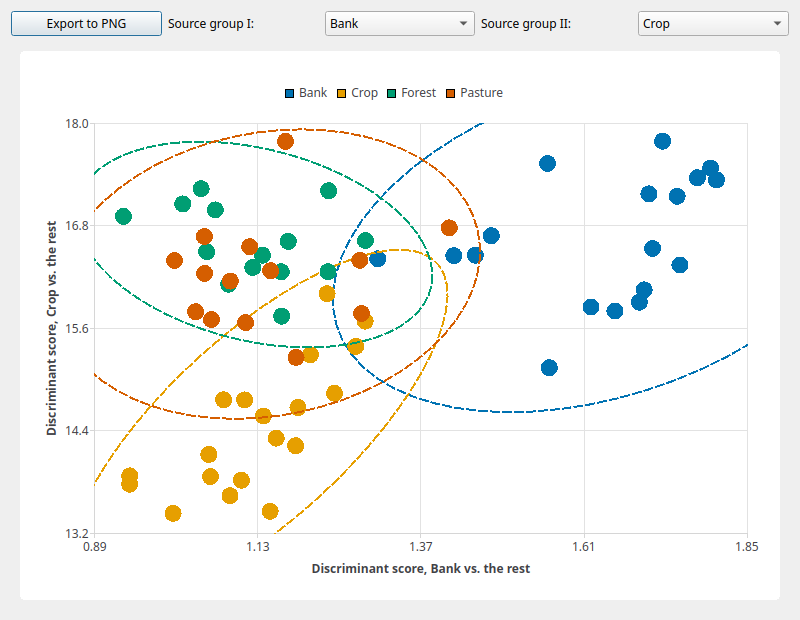
\includegraphics[width=0.46\textwidth]{Figures/Multiway-Scatter-Bank-Crop.png} &
        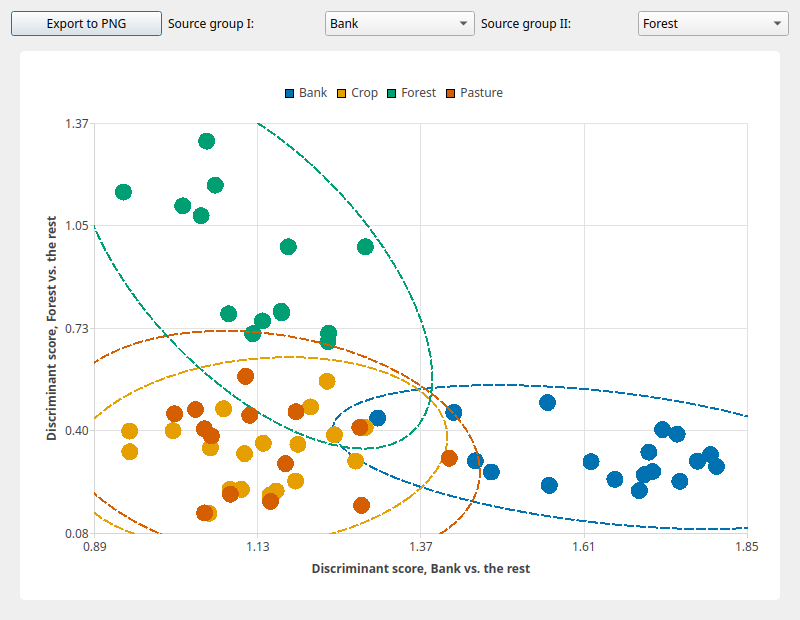
\includegraphics[width=0.46\textwidth]{Figures/Multiway-Scatter-Bank-Forest.png} \\
        c) & d) \\
        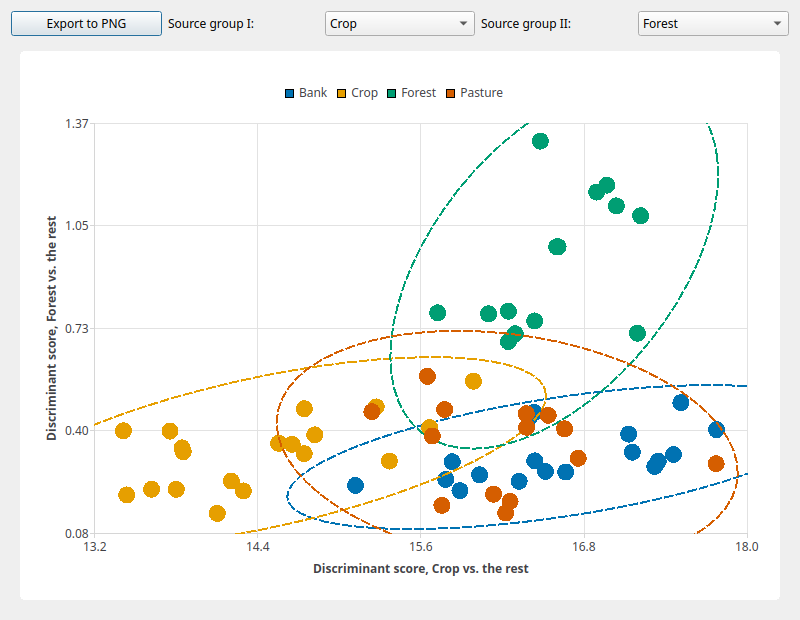
\includegraphics[width=0.46\textwidth]{Figures/Multiway-Scatter-Crop-Forest.png} &
        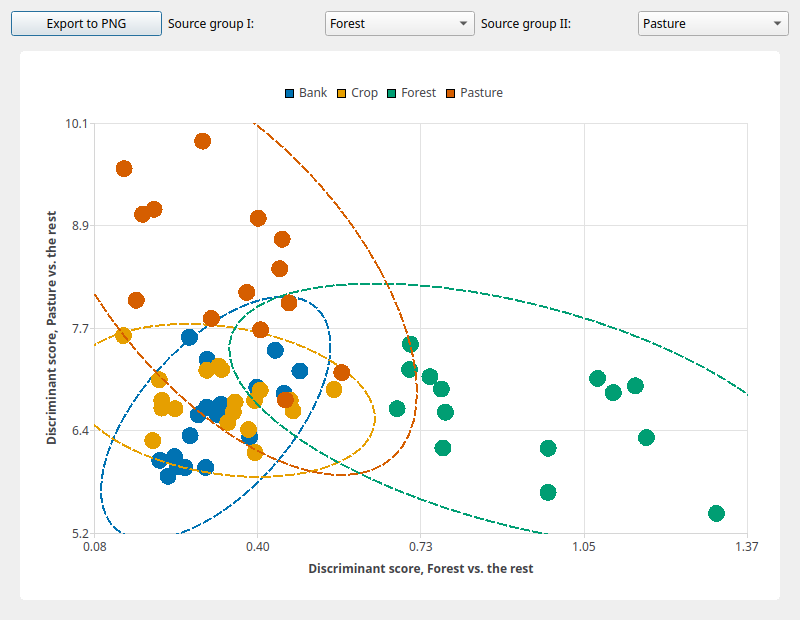
\includegraphics[width=0.46\textwidth]{Figures/Multiway-Scatter-Forest-Pasture.png}
    \end{tabular}
    \caption{Discriminant scores of the source samples on the discriminant functions of a) Bank and Crop, b) Bank and Forest, c) Crop and Forest, and d) Forest and Pasture, computed with the seven selected constituents.}
    \label{fig:Multiway-DFA-scatter-plots}
\end{figure}
\FloatBarrier

Finally, the sixth panel contains the eigenvectors obtained by maximizing the separation between each source group and the rest: the weight of each selected constituent in each group's discriminant function. Click the table button~
\includegraphics[width=0.5cm]{Figures/table.png} on the side of the panel to view the eigenvectors in tabular form (Fig.~\ref{fig:Multiway-eigenvectors}).

\begin{figure}[ht]
    \centering
    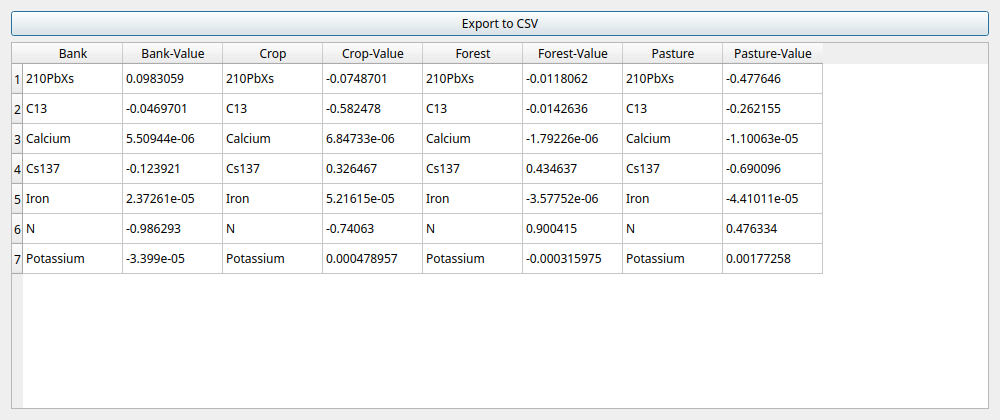
\includegraphics[width=\textwidth]{Figures/Multiway-DFA-eigenvectors.png}
    \caption{Estimated eigenvectors based on maximizing the separation of samples in each source group from all other samples.}
    \label{fig:Multiway-eigenvectors}
\end{figure}
\FloatBarrier

The seventh panel is the confusion matrix. Each source sample is classified into the source group it most resembles in the selected constituents, and the table counts the results. Each row is a true source group and each column the group assigned, and the last column gives the percentage of the group's samples classified correctly. Click the table button~
\includegraphics[width=0.5cm]{Figures/table.png} to view it (Fig.~\ref{fig:confusion-matrix}).

The classification is linear discriminant analysis with equal prior probabilities and leave-one-out cross-validation, as in Sed\_SAT \citep{gormansanisaca2017determining}. Each sample in turn is left out. The group means and the pooled within-group covariance matrix are computed from the remaining samples, and the sample is assigned to the group whose mean is nearest in Mahalanobis distance. Because the sample being classified does not contribute to the statistics, the percentages are an honest measure of how well the constituents would classify a new sample.

A perfect set of tracers gives counts only on the diagonal. Off-diagonal counts show which groups the tracers confuse. In the example (Fig.~\ref{fig:confusion-matrix}), most misclassifications are between Crop and Pasture, so their individual contributions will be less certain than their combined one; if they cannot be separated, consider combining them into one source. The confusion matrix measures separation by the discriminant function, not by the mixing model; Source Verification (Section~\ref{sec:tools-uncertainty}) checks the same question with the fingerprinting itself, and the two need not agree exactly.

\begin{figure}[ht]
    \centering
    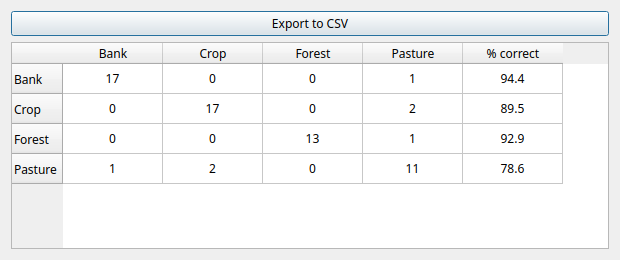
\includegraphics[width=0.7\textwidth]{Figures/DFA_confusion_matrix.png}
    \caption{Leave-one-out confusion matrix of the source samples of the example data, with the seven constituents selected in step~4: rows are the true source groups, columns the groups assigned.}
    \label{fig:confusion-matrix}
\end{figure}
\FloatBarrier


\section{Fingerprinting}\label{sec:lmmle}
The Levenberg--Marquardt Maximum Likelihood Estimation (LMMLE) is the simplest fingerprinting method implemented in SedSAT3. LMMLE uses the Levenberg--Marquardt optimization algorithm to maximize the log-likelihood in Eq.~\eqref{eq:loglikelihood-eqstd}. The transformation function $g$ is assumed to be log-normal, and the scale factor $\sigma$ of the log-normal distribution is assumed to be the same for all elements.

The modeled target sample elemental profile $\mathbf{C}$ is calculated as the arithmetic average of the elemental profiles of all samples in each source group (Eq.~\eqref{eq:y_avg}).

To perform LMMLE, select \textbf{Tools}$\rightarrow$\textbf{Deterministic Sediment Fingerprinting}$\rightarrow$\textbf{5-Fingerprinting} from the tools window. Fingerprinting uses every constituent marked \textit{Yes} in \textbf{Settings}$\rightarrow$\textbf{Constituent Properties} and every sample marked \textit{Yes} in \textbf{Settings}$\rightarrow$\textbf{Include/Exclude Samples}. Each included isotope also needs its base element included (Section~\ref{sec:importing_data}).

Checking \textit{Apply size and organic correction} applies the previously fitted size and organic matter correction to the source samples; the most recently fitted correction model is used. The correction is applied to the elements, particle size, and/or organic matter according to the selections in \textbf{Settings}$\rightarrow$\textbf{Organic Matter and Size Correction}. If no correction has been performed yet, an error message will prompt you to perform one. You can either uncheck the correction option and proceed without it, or perform the correction and then return to this tool.

Choose the target sample you have been working with (since the bracketing test) from the \textbf{Target Sample} drop-down menu. The \textit{Softmax} option maps the source contributions from the $[0, 1]$ domain to the $[-\infty, \infty]$ domain through the softmax transformation:
\begin{equation}
    x_i = \frac{e^{\zeta_i}}{\sum_{j=1}^{n} e^{\zeta_j}}
\end{equation}
When this option is selected, the optimization is performed in terms of $\zeta$ values rather than $x$ values. The softmax transformation implicitly enforces the constraint that the contributions sum to 1.0 (Eq.~\eqref{eq:sum}), and searching in the unbounded domain is more efficient than searching in $[0, 1]$.

Click the \textbf{Ok} button at the bottom of the form. The progress window will show the mean squared error (MSE) as the Levenberg--Marquardt iterations proceed; it closes when the analysis ends. After convergence, the result window will appear. It contains four panels.

The first panel shows the inferred source contributions. Click the graph button~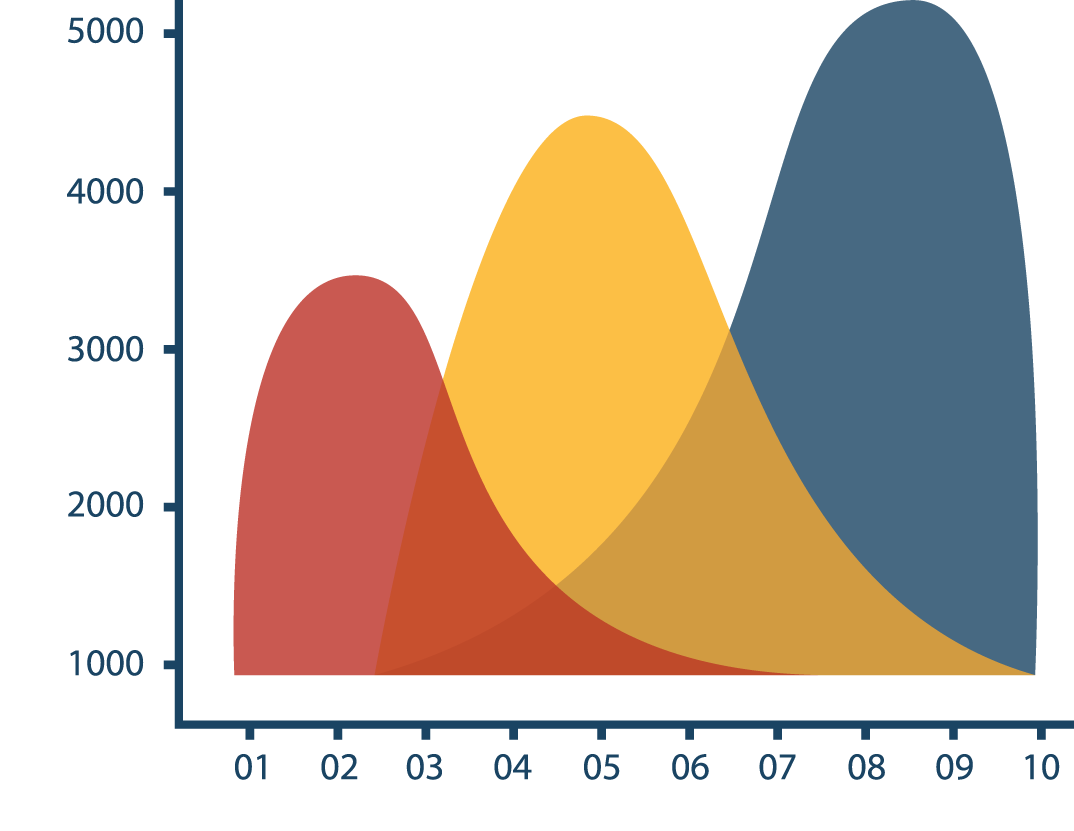
\includegraphics[width=0.5cm]{Figures/Graph.png} on the side of the panel to view the results as a pie chart (Fig.~\ref{fig:contribution_pie_chart}).

\begin{figure}[ht]
    \centering
    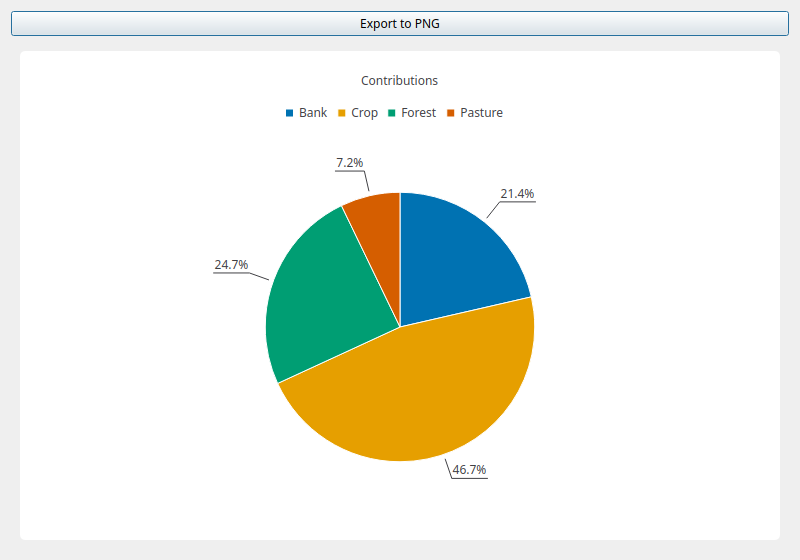
\includegraphics[width=\textwidth]{Figures/Contribution_Pie_Chart.png}
    \caption{Source contributions obtained from the LMMLE method}
    \label{fig:contribution_pie_chart}
\end{figure}
\FloatBarrier

The second panel shows the modeled target sample elemental profile, $\mathbf{C}$. The third panel shows the modeled and observed elemental profiles side by side, which you can use to evaluate how closely the mixture of source contributions reproduces the observed target sample profile. Click the graph button~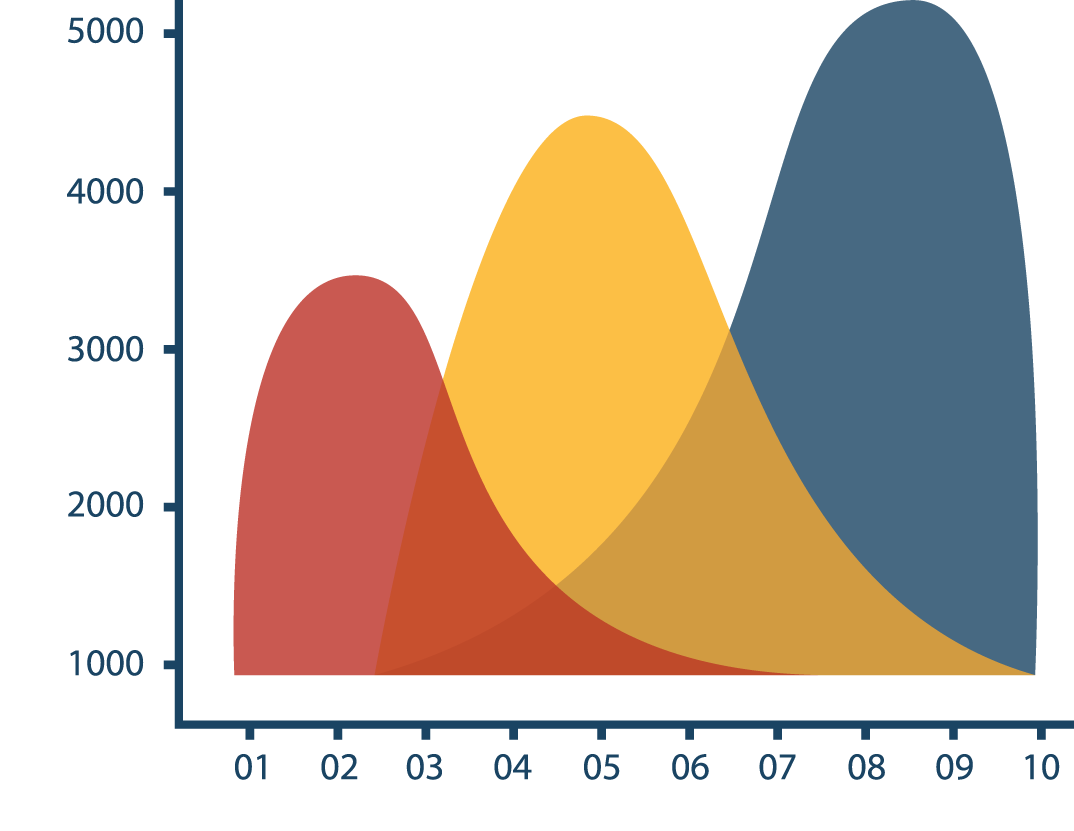
\includegraphics[width=0.5cm]{Figures/Graph.png} on the side of the panel to view the comparison graphically (Fig.~\ref{fig:LMMLE_modeled_vs_measured}). The modeled value is the larger circle and the observed value the smaller one drawn on top; where they agree closely, the modeled value shows as a ring around the observed one.

\begin{figure}[ht]
    \centering
    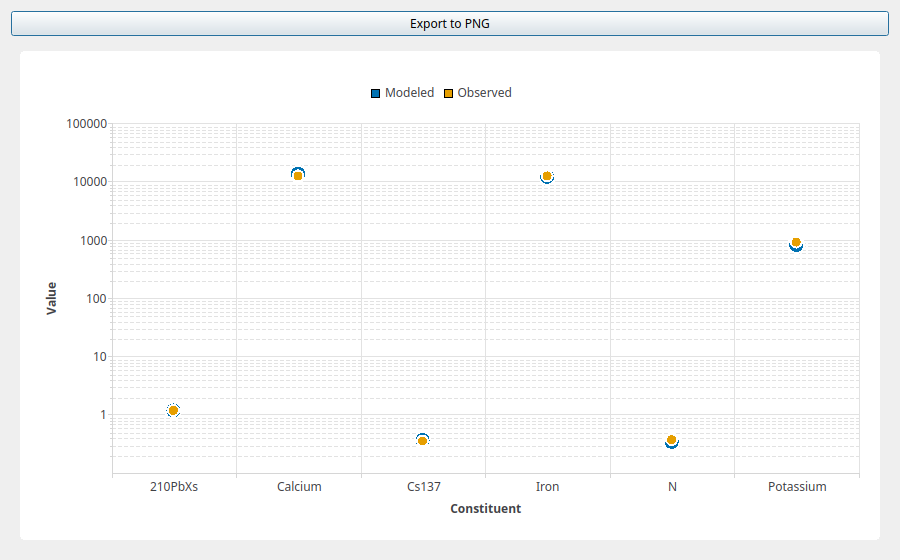
\includegraphics[width=\textwidth]{Figures/LMMSE_modeled_vs_measured.png}
    \caption{Modeled vs.\ observed elemental profiles}
    \label{fig:LMMLE_modeled_vs_measured}
\end{figure}
\FloatBarrier

The fourth panel shows the modeled vs.\ measured isotope ratios, if any constituents in the analysis are isotopes.

\section{Fingerprinting (Batch)}\label{sec:fingerprinting-batch}
The batch fingerprinting tool runs Levenberg--Marquardt maximum likelihood fingerprinting on all target samples simultaneously rather than one at a time. It is intended for studies in which multiple target samples are analyzed under identical settings, and it saves the effort of opening, configuring, and saving the fingerprinting tool for each sample individually.

\begin{tcolorbox}[colback=yellow!10,colframe=yellow!50!black,title=Note]
The batch tool uses one constituent selection and one sample selection for every target sample. Use it only when the same pre-processing decisions (outlier exclusion, bracketing, element selection from DFA) suit all target samples. Any element that does not pass bracketing for at least one target sample should be excluded for all of them before the batch is run; otherwise, the affected samples may produce misleading contributions.

The organic matter and size correction, when applied, is computed for each target sample separately: the sources are corrected to the organic matter content and particle size of the target sample being analyzed, using the regressions of step~2. In the steps that precede the batch, however, the correction is based on the one target sample chosen in each form (for example, the DFA of step~4). If the target samples differ greatly in organic matter content or particle size, check that the constituents selected with one target sample are also suitable for the others, for example by repeating step~4 with a target sample from each end of the range.
\end{tcolorbox}

To run the batch analysis, select \textbf{Tools}$\rightarrow$\textbf{Deterministic Sediment Fingerprinting}$\rightarrow$\textbf{6-Fingerprinting (Batch)} from the tools window. In the form that appears, choose whether to apply the OM and size correction to the source samples, and whether to use the softmax transformation (see Section~\ref{sec:lmmle} for details on what each option does). Click \textbf{Ok} and wait for the analysis to complete. Processing time depends on the number of target samples, the number of source groups, and the number of elements retained in the analysis.

The batch version of LMMLE reports less diagnostic detail than the single-sample version: only the estimated source contributions for each target sample are returned, without the modeled-versus-observed elemental profiles, MSE history, or modeled isotope ratios. If you need those diagnostics for a particular target sample, re-run the single-sample fingerprinting tool (Section~\ref{sec:lmmle}) on that sample.

The result panel contains one row per target sample and one column per source group. Click the graph button~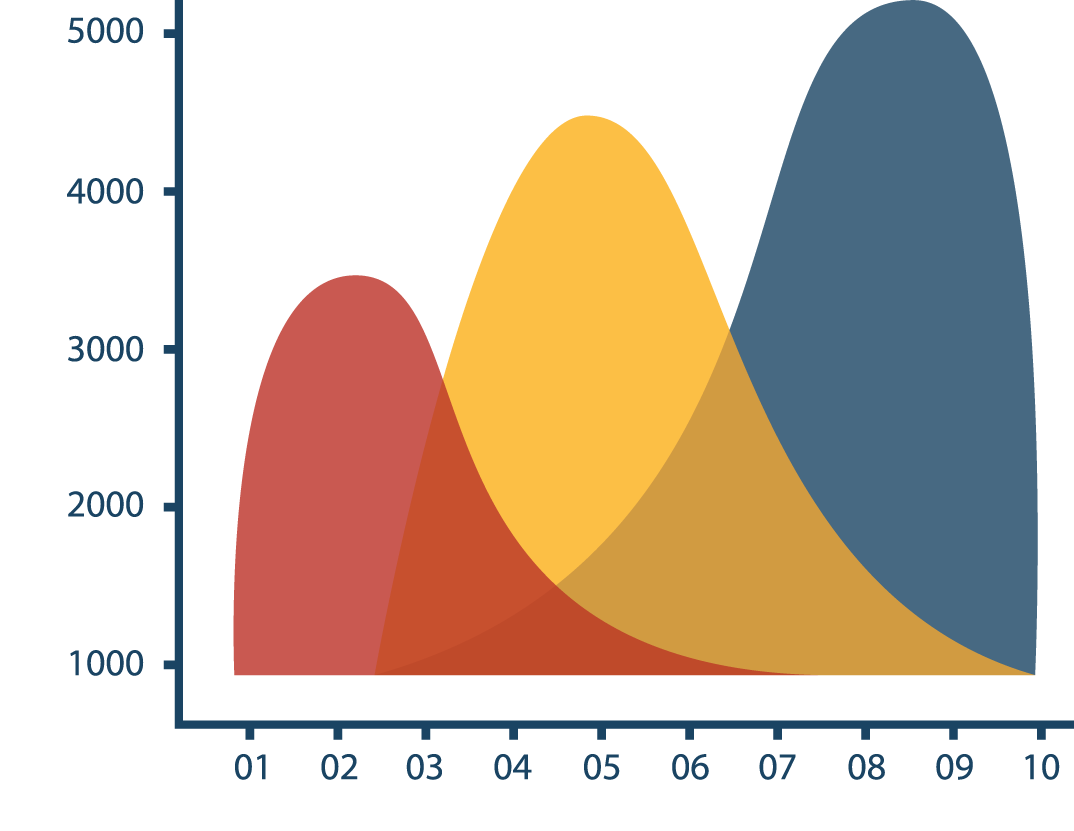
\includegraphics[width=0.5cm]{Figures/Graph.png} on the side of the panel to view the contribution of each source to each target sample as a stacked bar chart (Fig.~\ref{fig:LM-Batch-results-graph}), or the table button~
\includegraphics[width=0.5cm]{Figures/table.png} to view the same results in tabular form (Fig.~\ref{fig:LM-Batch-results-table}). The table can be exported to a CSV file using the \textbf{Export to CSV} button at the top of the window, which is useful for downstream analysis or for combining results across batches.

\begin{figure}[ht]
    \centering
    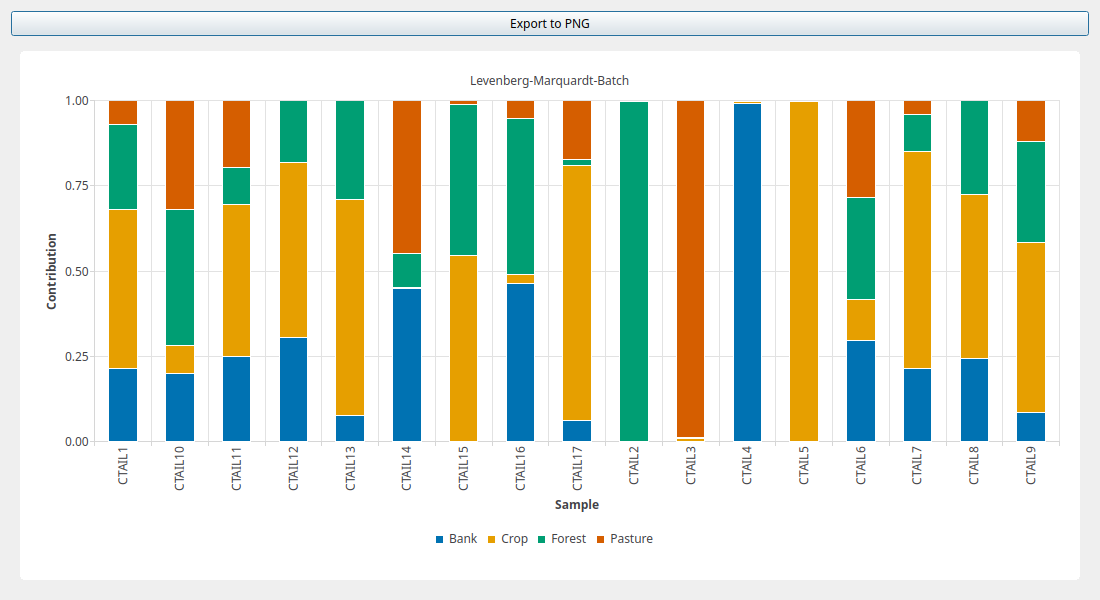
\includegraphics[width=\textwidth]{Figures/LL-batch-graph.png}
    \caption{Stacked bar chart of Levenberg--Marquardt batch fingerprinting results, showing the source contributions to each target sample.}
    \label{fig:LM-Batch-results-graph}
\end{figure}
\FloatBarrier

\begin{figure}[ht]
    \centering
    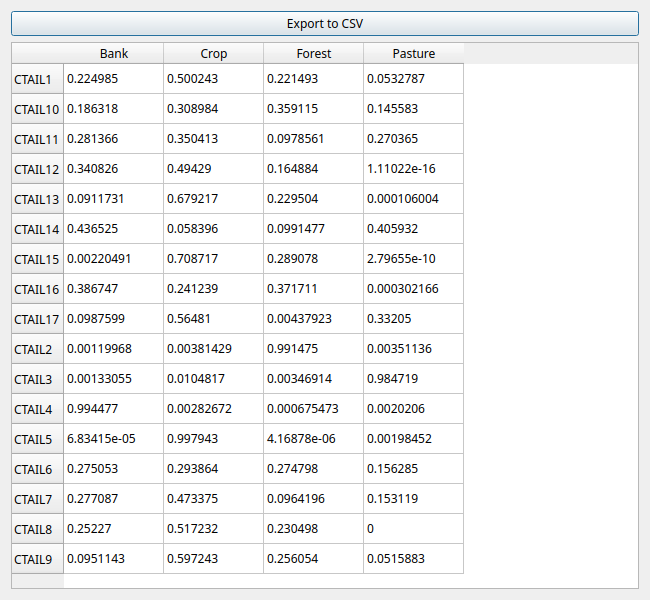
\includegraphics[width=0.46\textwidth]{Figures/LL-batch-table.png}
    \caption{Levenberg--Marquardt batch results in tabular format.}
    \label{fig:LM-Batch-results-table}
\end{figure}
\FloatBarrier

\chapter{Bayesian Sediment Fingerprinting}\label{chap:bayesian}
This chapter covers the Bayesian fingerprinting method implemented in SedSAT3. The pre-analysis steps required for Bayesian fingerprinting---namely, \textit{Outlier Analysis}, \textit{Organic Matter and Particle Size Correction}, \textit{Bracketing Analysis}, and \textit{Stepwise Discriminant Function Analysis}---were presented in the previous chapter. The focus here is on the Bayesian sediment fingerprinting procedure, which produces the final results of the analysis.

\section{Bayesian Chemical Mass Balance Analysis}\label{sec:bayesian_cmb}
As discussed in Section~\ref{sec:basic_concepts_bayesian}, sediment fingerprinting is subject to several sources of uncertainty, including (but not limited to) measurement error, lack of representativeness of source samples, the presence of unidentified sources, and equifinality. Rather than producing point estimates as the maximum likelihood approach does, the Bayesian approach yields a full probability distribution for each source contribution, allowing these uncertainties to be quantified.

To perform Bayesian fingerprinting, select \textbf{Tools}$\rightarrow$\textbf{Bayesian Sediment Fingerprinting}$\rightarrow$\textbf{5-Bayesian Chemical Mass Balance Analysis} from the tools window. Steps 1 to 4 of this menu are the same tools as in Chapter~\ref{chap:deterministic}.

The settings in the central form are:

\begin{itemize}
    \item \textbf{Apply size and organic matter correction:} whether to perform the analysis on the elemental profiles corrected for particle size and organic matter content. Note that the size and organic matter correction step (Section~\ref{sec:sizeandorganiccorrection}) must have been performed beforehand for this option to take effect.
    \item \textbf{Dissolve Chains:} when checked, MCMC chains with significantly lower posterior probability are discarded during sampling and replaced by chains with higher posterior probability. This improves the convergence speed of the algorithm.
    \item \textbf{Number of chains:} the number of MCMC chains run in parallel (default 8). The chains run on separate processor cores, so up to the number of cores more chains cost little extra time. More chains explore the posterior from more starting points, which makes it easier to judge convergence. The default suits a typical desktop computer.
    \item \textbf{Number of samples:} the total number of MCMC samples to generate (default 100{,}000). Typically, 100{,}000 samples or more are required for convergence.
    \item \textbf{Random seed:} leave blank to have one chosen. The seed used is shown in the name of the results and written on the first line of the samples file; entering it again repeats the run exactly.
    \item \textbf{Sample:} the label of the target sample to be analyzed.
    \item \textbf{Samples file name:} the text file in which the MCMC samples will be saved.
    \item \textbf{Samples to be discarded (burn-in):} the number of samples to discard from the beginning of the chains (default 20{,}000, that is, 20\% of 100{,}000).
\end{itemize}

After setting the parameters, click \textbf{Ok} to start the analysis. The runtime depends on the number of samples requested.

The progress window (Fig.~\ref{fig:MCMC-progress}) provides diagnostic information that can help you tune the MCMC sampling parameters.

\begin{figure}[ht]
    \centering
    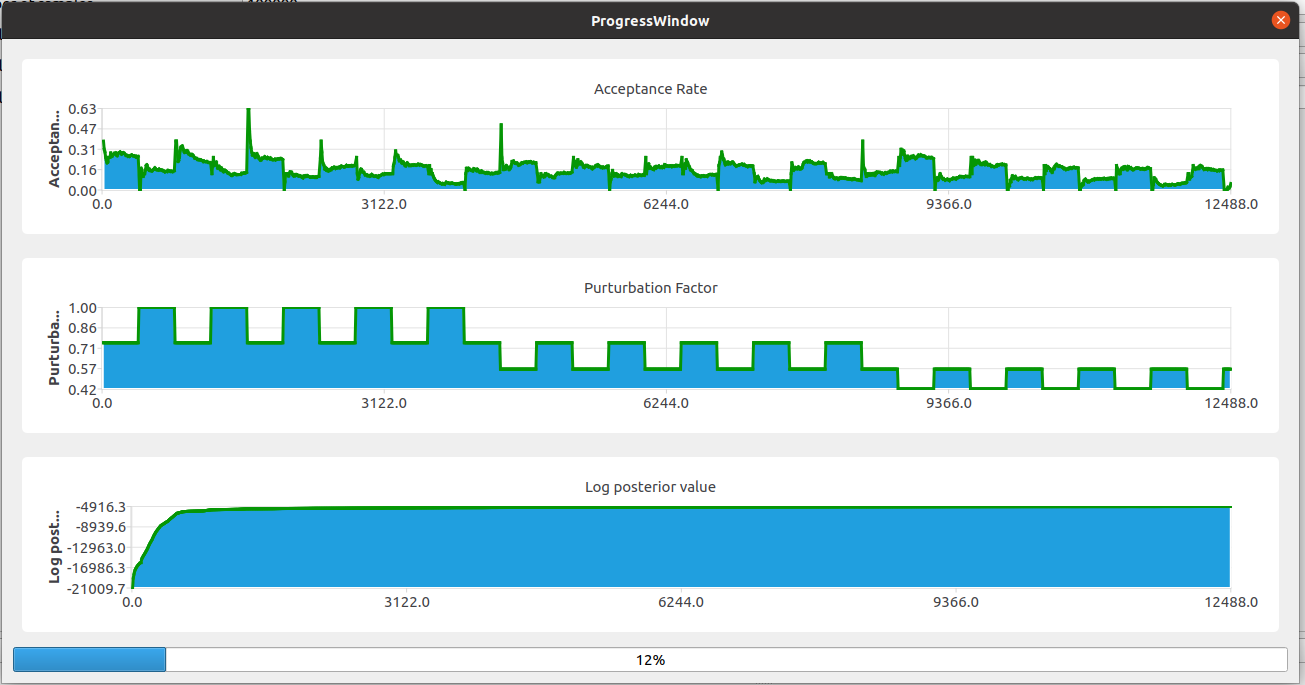
\includegraphics[width=\textwidth]{Figures/MCMC_progress.png}
    \caption{Progress window of the Bayesian chemical mass balance analysis.}
    \label{fig:MCMC-progress}
\end{figure}
\FloatBarrier

The top panel shows the average acceptance rate (the fraction of proposed samples that are accepted). The middle panel shows the perturbation factor, which is automatically adjusted to maintain an acceptance rate of approximately 15\%. The bottom panel shows the maximum value of the posterior numerator (Eq.~\eqref{eq:Bayesian-Prop}). Initially, this value is low because the samples are far from the maximum-likelihood region; as the algorithm proceeds, the value rises and eventually stabilizes. A reasonable burn-in length can be chosen as the number of samples it takes for this curve to stabilize.

Once MCMC sampling is complete, a result window appears containing five panels.

The first panel contains the MCMC samples for every estimated parameter: source contributions, the $\mu$ and $\sigma$ parameters of the log-normal distributions assumed for the elemental content of each source group, and the error standard deviations. Click the graph button~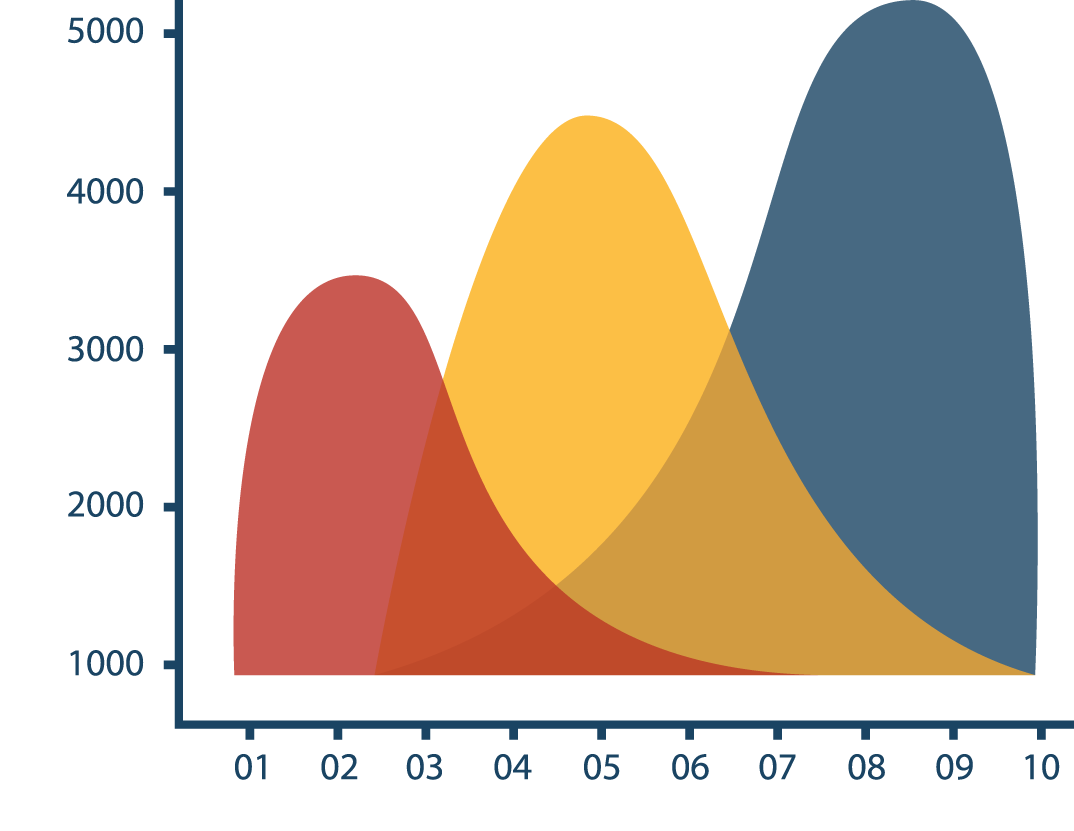
\includegraphics[width=0.5cm]{Figures/Graph.png} to visualize the samples (Fig.~\ref{fig:MCMC-samples}), and use the drop-down menu at the top of the graph to switch between parameters. Inspect these plots to assess convergence: after convergence, the samples fluctuate around a stable level with no trend, and the burn-in should end after the initial trend. For example, in Fig.~\ref{fig:MCMC-samples} the Bank and Crop contribution samples settle after approximately 15{,}000 to 20{,}000 samples, so the default burn-in of 20{,}000 is adequate. If the samples still drift at the end of the run, increase the number of samples (and the burn-in) and run again; with too few samples, the plot looks like scattered noise with no stable level.

\begin{figure}[ht]
    \centering
    \begin{tabular}{cc}
        a) & b) \\
        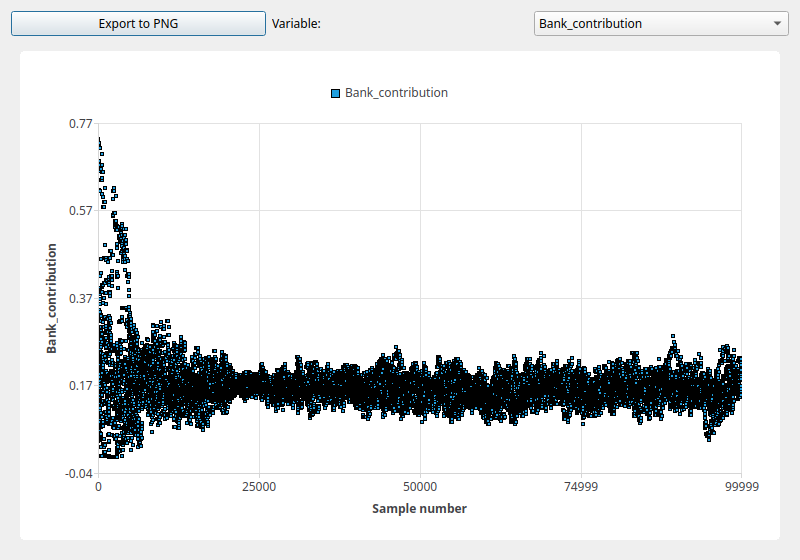
\includegraphics[width=0.46\textwidth]{Figures/MCMC_Samples_Bank.png} &
        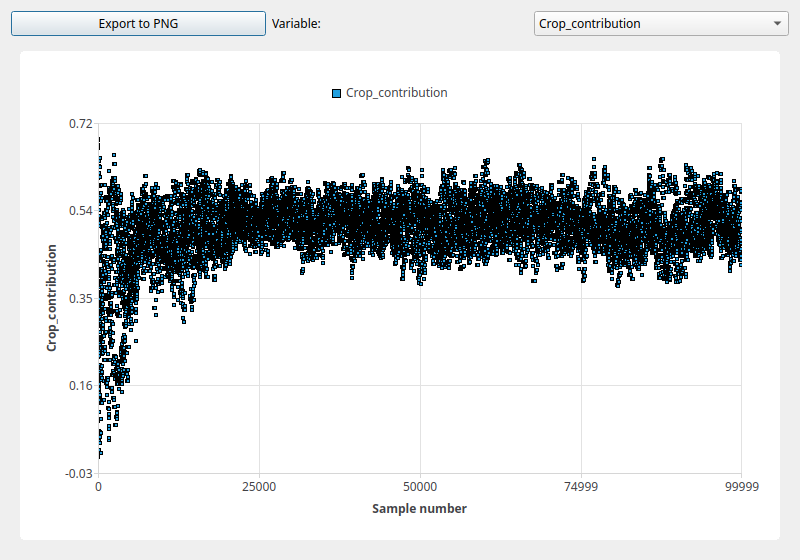
\includegraphics[width=0.46\textwidth]{Figures/MCMC_samples_crop.png}
    \end{tabular}
    \caption{MCMC samples of a) the Bank contribution and b) the Crop contribution for target sample CTAIL1 of the example data (8 chains, 100{,}000 samples).}
    \label{fig:MCMC-samples}
\end{figure}
\FloatBarrier

The second panel shows the posterior distributions estimated from the samples. Click the graph button~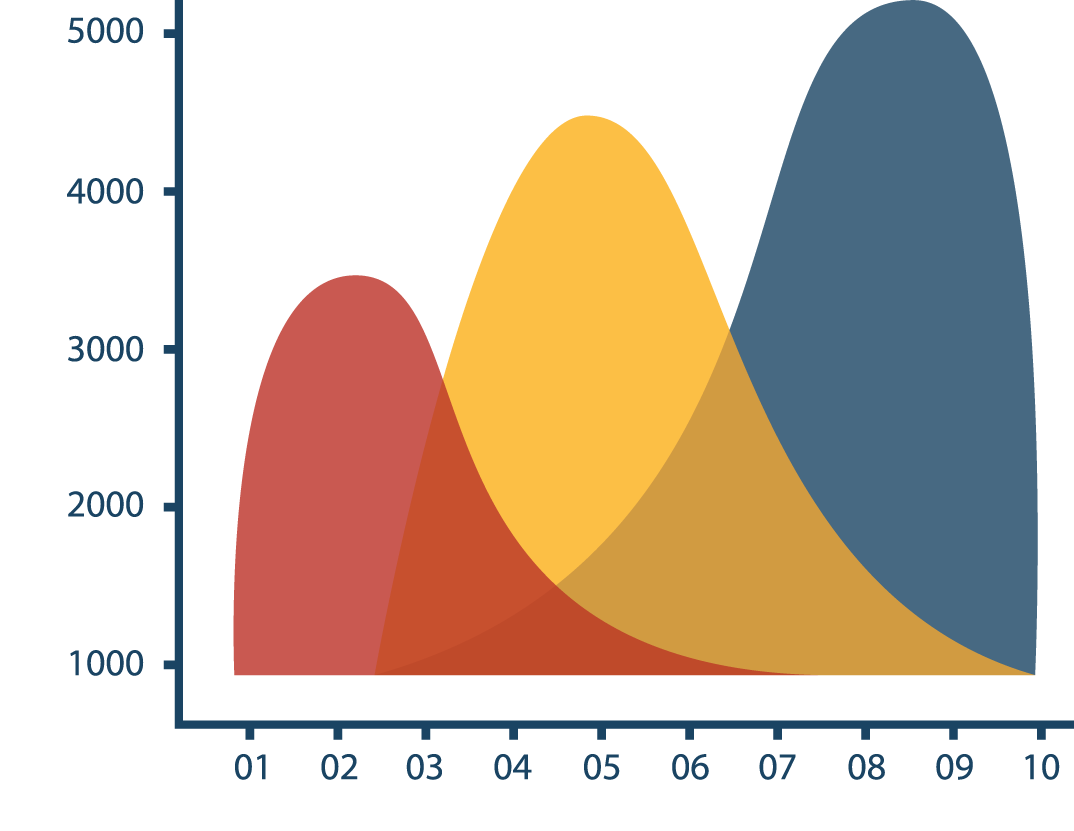
\includegraphics[width=0.5cm]{Figures/Graph.png} to view the posterior distributions for all parameters (Fig.~\ref{fig:MCMC-distributions}).

\begin{figure}[ht]
    \centering
    \begin{tabular}{cc}
        a) & b) \\
        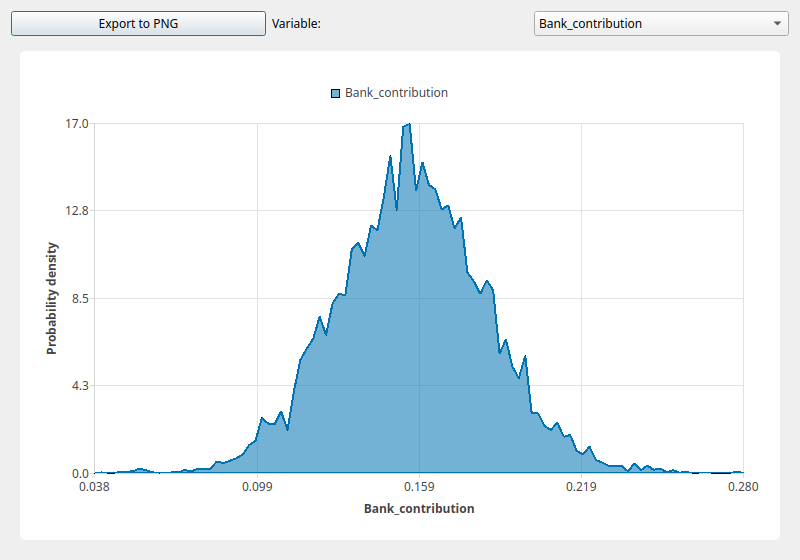
\includegraphics[width=0.46\textwidth]{Figures/MCMC_Bank_Distribution.png} &
        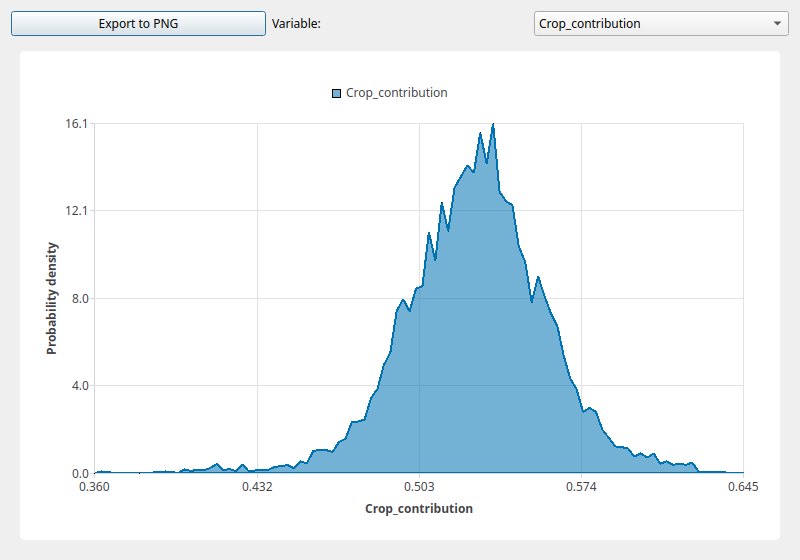
\includegraphics[width=0.46\textwidth]{Figures/MCMC_crop_distribution.png}
    \end{tabular}
    \caption{Visualization of the posterior distribution for a) bank contribution and b) crop contribution.}
    \label{fig:MCMC-distributions}
\end{figure}
\FloatBarrier

The third panel contains the 95\% credible intervals for the source contributions: the range within which each source contribution lies with 95\% probability (Fig.~\ref{fig:MCMC-credible-interval}). In addition to the lower and upper bounds of the credible interval, the panel also reports the expected value (mean) and median of each posterior distribution.

Click the table button~
\includegraphics[width=0.5cm]{Figures/table.png} on the side of the panel to view the intervals in tabular form, or the graph button~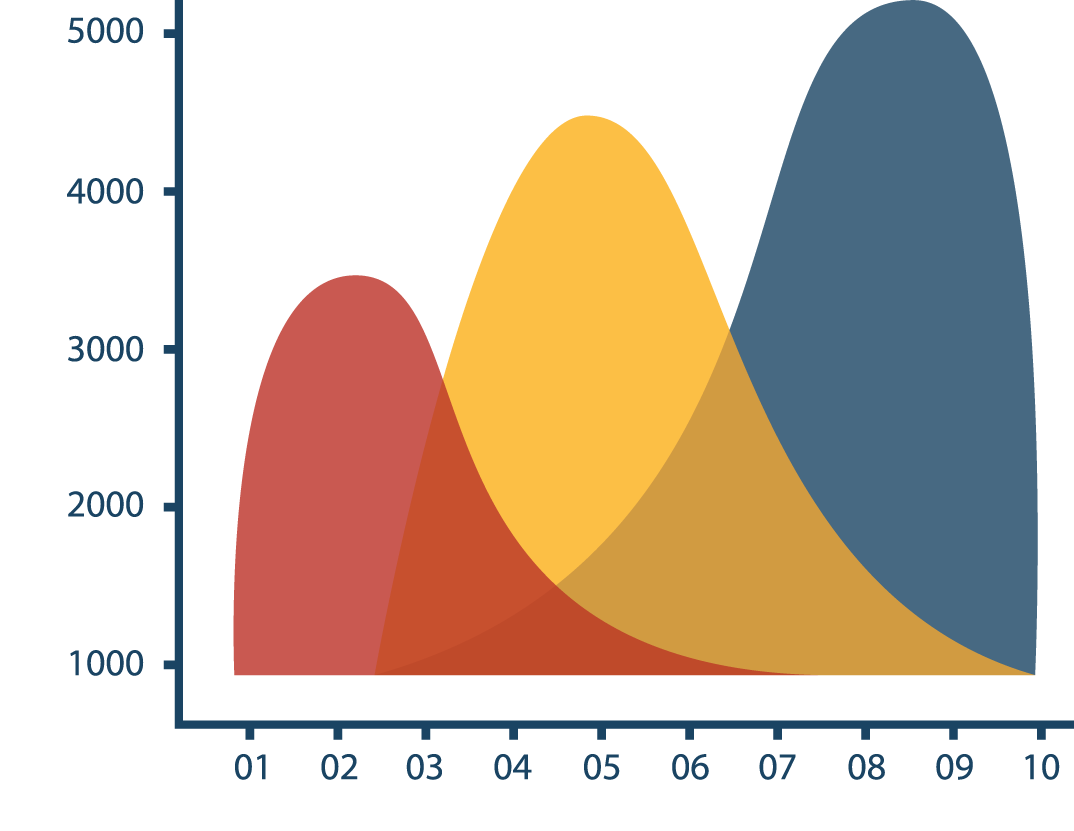
\includegraphics[width=0.5cm]{Figures/Graph.png} to view them graphically.

\begin{figure}[ht]
    \centering
    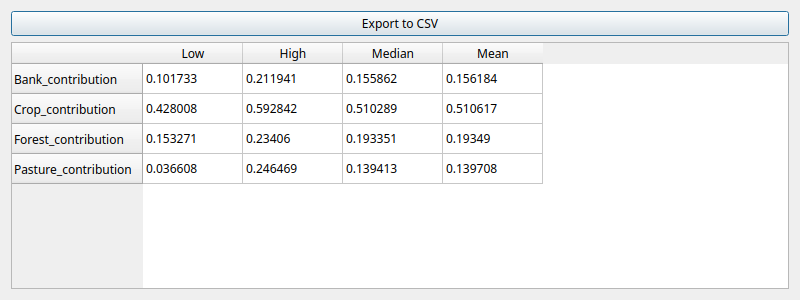
\includegraphics[width=\textwidth]{Figures/MCMC-credible-intervals.png}
    \caption{Credible intervals for source contributions.}
    \label{fig:MCMC-credible-interval}
\end{figure}
\FloatBarrier

The fourth panel contains the posterior predictive distribution of elemental content in the target sample. Click the graph button~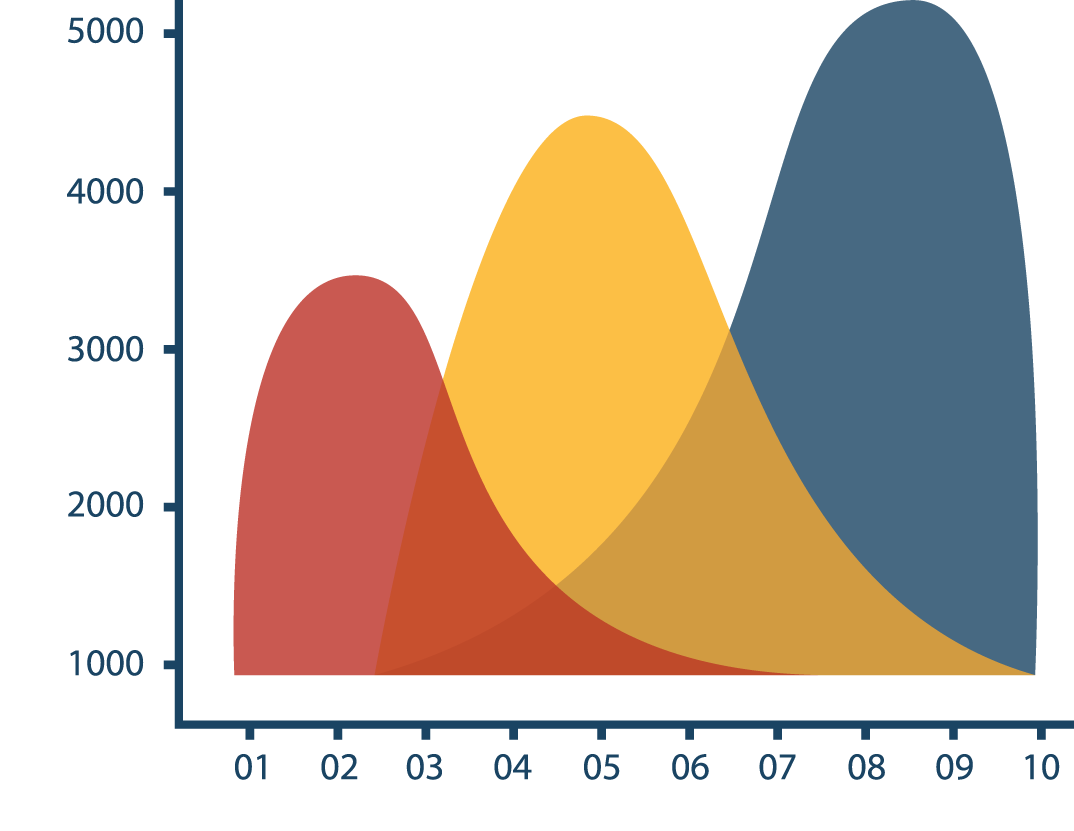
\includegraphics[width=0.5cm]{Figures/Graph.png} to view the distributions graphically. Use the drop-down menu at the top of the graph to display the predicted distribution for each element (Fig.~\ref{fig:MCMC-posterior-elemental-content}). The distribution is constructed by computing the modeled target elemental profile for each MCMC sample. The vertical dashed line on each graph indicates the measured concentration in the target sample.

These plots show how well the inferred mixture of sources reproduces each tracer. When the measured value (dashed line) lies within the predicted distribution, the tracer is consistent with the model. When it lies in the tail or outside the distribution, the model cannot reproduce that tracer with the sources given. Common reasons are that the tracer is not conservative (its concentration changes during erosion and transport), that a source is missing from the analysis, that the size and organic matter correction does not suit the tracer, or that the tracer failed, or nearly failed, the bracket test. Consider excluding such a tracer and running the analysis again, and compare the contributions; Section~\ref{sec:interpretation} gives further guidance.

\begin{figure}[ht]
    \centering
    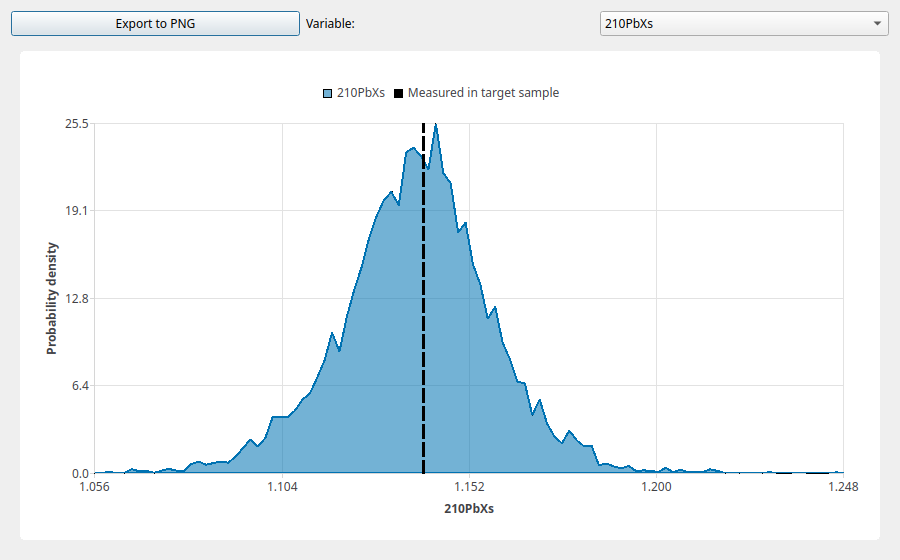
\includegraphics[width=\textwidth]{Figures/MCMC_Posterior_Elemental_Contents.png}
    \caption{Posterior predictive distribution of elemental content in the target sample.}
    \label{fig:MCMC-posterior-elemental-content}
\end{figure}
\FloatBarrier

The fifth panel contains the 95\% credible intervals for the predicted elemental content in the target sample. Click the table button~
\includegraphics[width=0.5cm]{Figures/table.png} on the side of the panel to view the intervals in tabular form, or the graph button~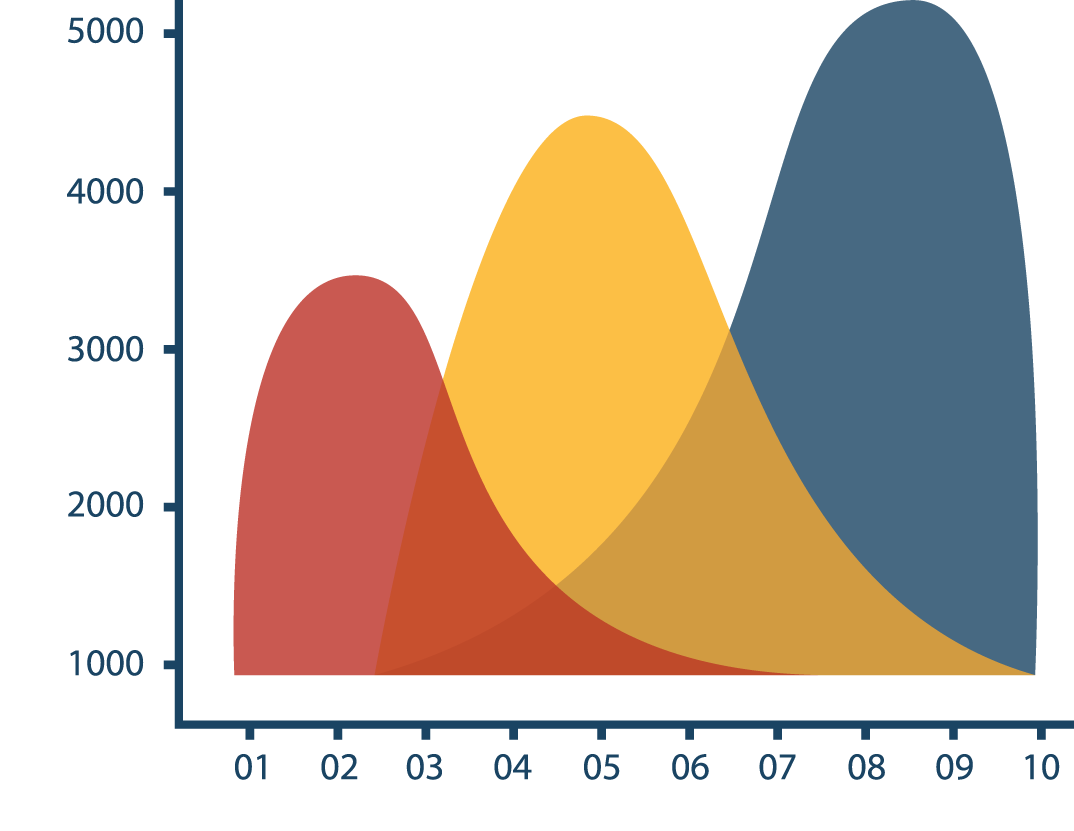
\includegraphics[width=0.5cm]{Figures/Graph.png} to view them graphically (Fig.~\ref{fig:MCMC-predicted-CI}). The graph shows each interval as a green box, with the median as a line, and the measured elemental content in the target sample as a black dot.

\begin{figure}[ht]
    \centering
    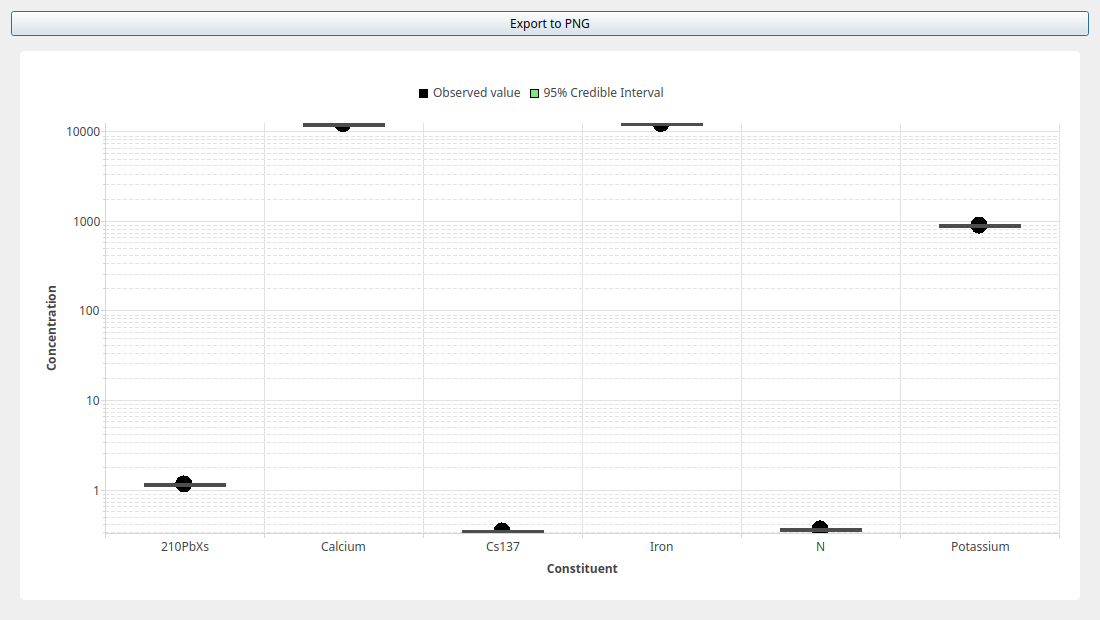
\includegraphics[width=\textwidth]{Figures/MCMC_predicted_credible_intervals.png}
    \caption{95\% credible intervals of the predicted constituent contents in the target sample (green boxes) and the measured contents (black dots).}
    \label{fig:MCMC-predicted-CI}
\end{figure}
\FloatBarrier
 The difference between the 95\% credible interval and the measured value provides insight into how well each element's content can be reproduced by the inferred combination of sources.

Panels six and seven contain analogous information to panels four and five, but for isotope ratios, when isotopes are included in the analysis.

\section{Bayesian Chemical Mass Balance Analysis (Batch)}\label{sec:bayesian-batch}
The batch version of the Bayesian Chemical Mass Balance tool runs Bayesian fingerprinting on all target samples in a single pass, avoiding the need to select and save each sample manually. Instead of displaying results as interactive tables and graphs, the analysis writes the outputs to text files that can be plotted in any spreadsheet or graphing application. The settings are identical to those described for the single-sample Bayesian Chemical Mass Balance Analysis (Section~\ref{sec:bayesian_cmb}). As in the deterministic batch (Section~\ref{sec:fingerprinting-batch}), one constituent and sample selection is used for every target sample, while the organic matter and size correction, when applied, is computed for each target sample from its own organic matter content and particle size; the note in that section applies here too.

To run the batch analysis, select \textbf{Tools}$\rightarrow$\textbf{Bayesian Sediment Fingerprinting}$\rightarrow$\textbf{Bayesian Chemical Mass Balance Analysis (Batch)} from the tools window.

\begin{tcolorbox}[colback=yellow!10,colframe=yellow!50!black,title=Note]
A large number of samples (at least 100{,}000, the default) is required for the chains to converge, and about 20\% of the total should be designated as burn-in (the default is 20{,}000). The analysis can take a substantial amount of time depending on the number of target samples, the number of source groups, the number of MCMC samples per chain, and your hardware. For long batches, consider running the analysis overnight or on a dedicated workstation.
\end{tcolorbox}

When the analysis is complete, a folder named after each target sample is created in the working folder (Fig.~\ref{fig:MCMC-folders}). The working folder is the folder of the project file last opened or saved, or, before the project is first saved, the folder of the Excel file imported; save the project first so that the results are written next to it. Each folder contains seven text files (Fig.~\ref{fig:MCMC-files}), and the MCMC samples file named in the form.

\begin{figure}[ht]
    \centering
    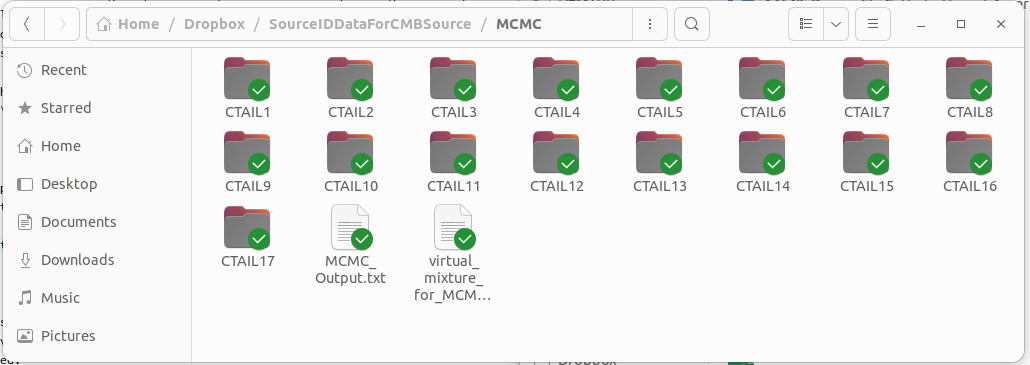
\includegraphics[width=\textwidth]{Figures/MCMC_folders.png}
    \caption{Folders created after running the batch Bayesian chemical mass balance analysis. One folder per target sample is created in the folder where the project was saved.}
    \label{fig:MCMC-folders}
\end{figure}
\FloatBarrier

\begin{figure}[ht]
    \centering
    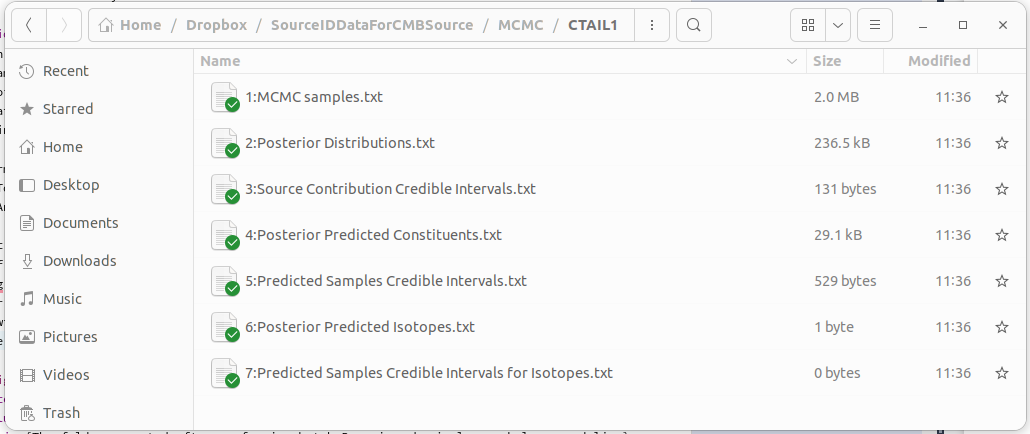
\includegraphics[width=\textwidth]{Figures/MCMC_files.png}
    \caption{The seven text files written for each target sample by the batch Bayesian chemical mass balance analysis.}
    \label{fig:MCMC-files}
\end{figure}
\FloatBarrier

The contents of each file are as follows:

\begin{itemize}
    \item \textbf{1\_MCMC samples.txt} --- contains all MCMC samples generated. Each column corresponds to one estimated parameter: the source contribution for each source group, the mean and standard deviation of each element in each source group, and the likelihood value for each parameter set.
    \item \textbf{2\_Posterior Distributions.txt} --- contains the MCMC samples converted into frequency distributions (histograms). Columns come in pairs: the first column of each pair contains the parameter values (bin centers), and the second contains the corresponding frequencies. For example, to plot the posterior distribution of \textit{Bank Contribution}, plot column B against column A; the next parameter follows in columns C and D, and so on.
    \item \textbf{3\_Source Contribution Credible Intervals.txt} --- contains the 95\% credible intervals for each parameter extracted from the posterior distribution (Fig.~\ref{fig:posterior-95-table}).

    \begin{figure}[ht]
        \centering
        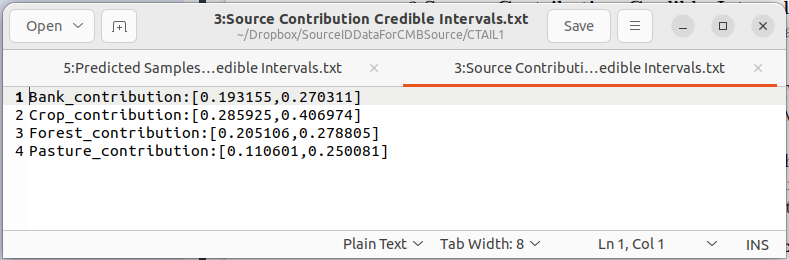
\includegraphics[width=\textwidth]{Figures/95p_CI_table.png}
        \caption{Excerpt from the 95\% credible interval file for model parameters.}
        \label{fig:posterior-95-table}
    \end{figure}
    \FloatBarrier

    \item \textbf{4\_Posterior Predicted Constituents.txt} --- contains the posterior predictive distributions of the target sample elemental concentrations, computed from the MCMC samples and presented as frequency distributions. Columns come in pairs (value, frequency); for example, to plot the predicted distribution of $^{210}\mathrm{Pb}$, plot column B against column A.

    \item \textbf{5\_Predicted Samples Credible Intervals.txt} --- contains the 95\% credible intervals of the predicted target sample elemental profile, derived from the predicted constituents in file 4 (Fig.~\ref{fig:posterior-95-predicted-table}).

    \begin{figure}[ht]
        \centering
        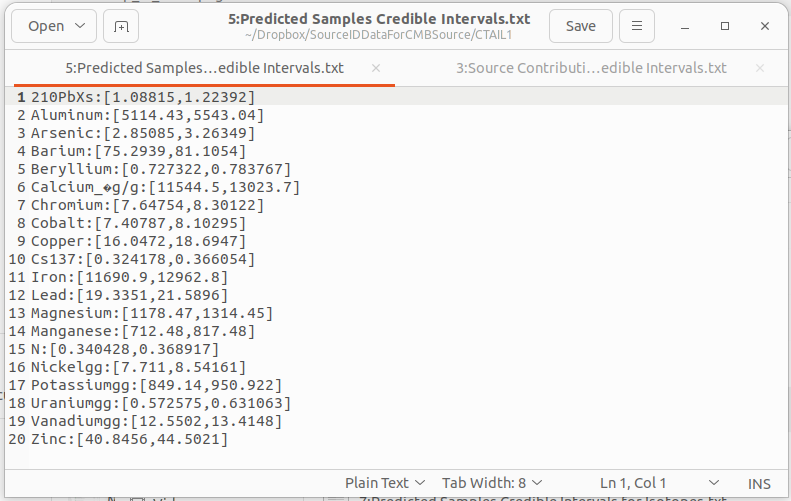
\includegraphics[width=\textwidth]{Figures/95p_CI_predicted.png}
        \caption{Excerpt from the 95\% credible interval file for predicted target sample elemental content.}
        \label{fig:posterior-95-predicted-table}
    \end{figure}
    \FloatBarrier

    \item \textbf{6\_Posterior Predicted Isotopes.txt} --- contains the posterior predictive distributions of the target sample isotope ratios, presented as frequency distributions. Columns come in pairs (value, frequency). This file is empty if no isotopes are included in the analysis.
    \item \textbf{7\_Predicted Samples Credible Intervals for Isotopes.txt} --- contains the 95\% credible intervals of the predicted target sample isotope ratios, derived from the isotope predictions in file 6.
\end{itemize}

\section{Interpreting the results}\label{sec:interpretation}
Sediment fingerprinting results should be judged by several lines of evidence rather than by one number. \citet{gormansanisaca2017determining} describe the steps of a study with the earlier Sed\_SAT tool, and \citet{collins2017sediment} review the method and the decisions it involves. With SedSAT3:
\begin{itemize}
    \item \textbf{Check the fit.} Compare the modeled and measured target sample (Section~\ref{sec:lmmle}, third panel; Section~\ref{sec:bayesian_cmb}, fourth and fifth panels). Tracers that the model cannot reproduce point to non-conservative behaviour, a missing source, or an unsuitable correction.
    \item \textbf{Check the tracers.} The selected tracers should pass the bracket test for the target sample and separate the source groups (step~4, Section~\ref{sec:multiway-dfa}). The confusion matrix of step~4 and source verification (Section~\ref{sec:tools-uncertainty}) show how well they classify the source samples.
    \item \textbf{Check the sensitivity.} Error analysis (Section~\ref{sec:tools-uncertainty}) shows how much the contributions depend on the particular source samples. Repeating the fingerprinting with a slightly different tracer selection, or with and without the organic matter and size correction, shows how much they depend on those choices.
    \item \textbf{Report the uncertainty.} The Bayesian credible intervals (Section~\ref{sec:bayesian_cmb}) combine the measurement and source variability. Contributions whose intervals are wide, or which change with the tracer selection, should be reported with that caution.
\end{itemize}

\chapter{Other Statistical Tools}\label{chap:other-tools}
This chapter describes the tools under \textbf{Tools}$\rightarrow$\textbf{Other Statistical Tools}. They are not steps of the fingerprinting workflow, but they help to explore the data and to decide which constituents and samples to include. The program groups them, in this order:
\begin{itemize}
    \item \textbf{Data exploration} (Section~\ref{sec:tools-exploration}): outliers, corrected profiles, correlation, distributions and normality;
    \item \textbf{Element selection} (Section~\ref{sec:tools-selection}): analysis of variance, auto-select and discriminant power;
    \item \textbf{Discriminant function analysis} (Section~\ref{sec:dfa-tools}): one vs.\ one, multi-way and one vs.\ the rest, each with a stepwise version;
    \item \textbf{Uncertainty and verification} (Section~\ref{sec:tools-uncertainty}): error analysis and source verification.
\end{itemize}

\section{Data exploration}\label{sec:tools-exploration}
\subsection{Outlier Analysis}
The same tool as step~1 of the fingerprinting menus; see Section~\ref{sec:outlier}.

\subsection{Correct based on size and organic matter}
Shows the source elemental profiles corrected for a chosen target sample, using the regressions of step~2; see Section~\ref{sec:view-corrected}.

\subsection{Elements' correlation matrix}\label{sec:tool-cormat}
The correlation between constituents within a source group is useful information when deciding which constituents to include in the fingerprinting analysis. Highly correlated tracers carry redundant information and can degrade the conditioning of the inverse problem.

The correlation between elements $j$ and $j'$ in source group $i$ is calculated as:
\begin{equation}
    r_{j,j'} = \frac{\sum_{k} (y_{j,k} - \bar{y}_j)(y_{j',k} - \bar{y}_{j'})}{\sqrt{\sum_{k} (y_{j,k} - \bar{y}_j)^2 \sum_{k} (y_{j',k} - \bar{y}_{j'})^2}}
\end{equation}
where $y_{j,k}$ and $y_{j',k}$ are the measured contents of elements $j$ and $j'$ in sample $k$ of the source group, and $\bar{y}_j$ and $\bar{y}_{j'}$ are the mean contents of elements $j$ and $j'$ in the source group.

To generate a correlation matrix, double-click \textbf{Tools}$\rightarrow$\textbf{Other Statistical Tools}$\rightarrow$\textbf{Data exploration}$\rightarrow$\textbf{Elements' correlation matrix} from the tools panel. In the form that appears:

\begin{itemize}
    \item Choose the source or target group from the \textbf{Source/Target group} drop-down.
    \item The \textbf{Threshold} field sets the value above which correlations are highlighted in the resulting matrix.
    \item Check \textit{Use only selected elements} to restrict the matrix to elements marked for inclusion in \textbf{Settings}$\rightarrow$\textbf{Constituent Properties}.
    \item Check \textit{Use only selected samples} to restrict the matrix to samples marked for inclusion in \textbf{Settings}$\rightarrow$\textbf{Include/Exclude Samples}.
    \item To run the correlation analysis on source elemental profiles adjusted for size, organic matter, or both, select the target sample on which the correction should be based.
\end{itemize}

Click \textbf{Ok}. A result window with one panel (Fig.~\ref{fig:correlation_matrix}) will appear. Click the table button~
\includegraphics[width=0.5cm]{Figures/table.png} to view the matrix (Fig.~\ref{fig:correlation_table}); correlations beyond the threshold are shown in red. The table can be exported to a CSV file.

\begin{figure}[ht]
    \centering
    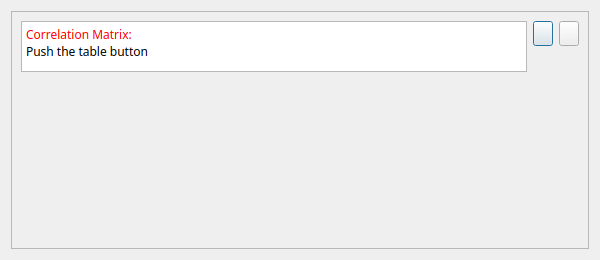
\includegraphics[width=0.46\textwidth]{Figures/Correlation_Matrix.png}
    \caption{Correlation matrix results.}
    \label{fig:correlation_matrix}
\end{figure}

\begin{figure}[ht]
    \centering
    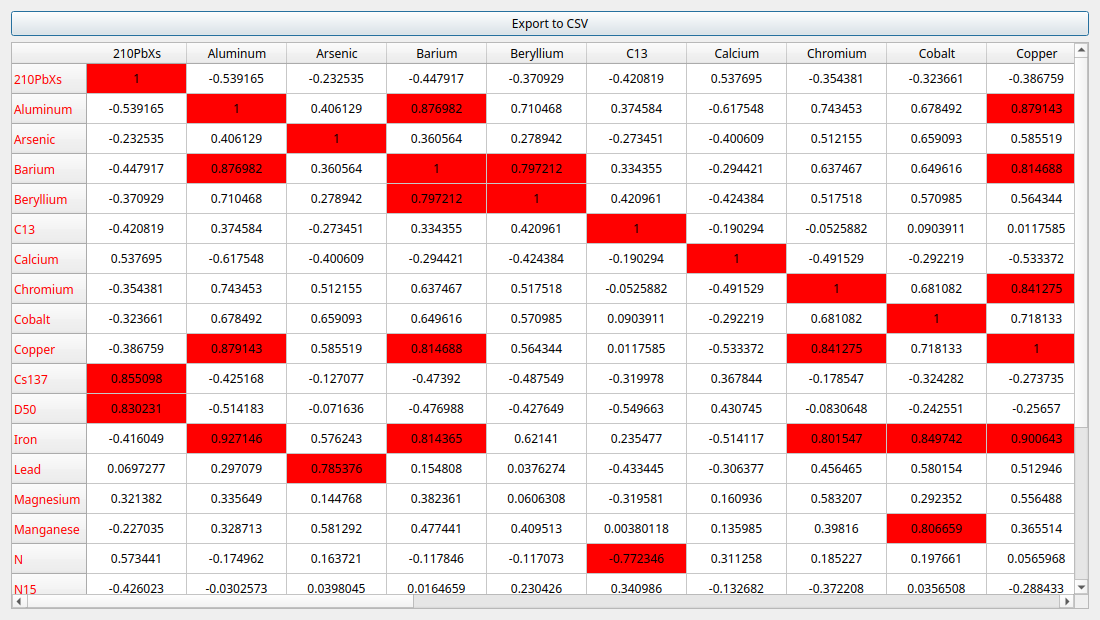
\includegraphics[width=\textwidth]{Figures/Correlation_Table.png}
    \caption{Correlation matrix in tabular form.}
    \label{fig:correlation_table}
\end{figure}
\FloatBarrier

Based on the correlation analysis, you can decide whether to eliminate any tracers from further analysis. Typically, a tracer is removed if it is highly correlated with another tracer across all source groups, since the two carry redundant information. To remove a tracer, go to \textbf{Settings}$\rightarrow$\textbf{Constituent Properties} and uncheck the element in the \textbf{Include in analysis} column. All correlation results you generate are retained in the results panel beneath the tools panel, so you can revisit them later.

\subsection{Distribution Fitting}\label{sec:tool-df}
The distribution fitting tool lets you visually inspect the frequency distribution of constituent content within a source group to determine whether it is better described by a normal or log-normal distribution. To run distribution fitting, select \textbf{Tools}$\rightarrow$\textbf{Other Statistical Tools}$\rightarrow$\textbf{Data exploration}$\rightarrow$\textbf{Distribution Fitting} from the tools menu. In the central form:

\begin{itemize}
    \item Choose the element and source group.
    \item Choose whether to include all samples or only the selected ones.
    \item Choose whether to fit the distribution to the raw data or to Box--Cox transformed elemental contents.
    \item To run the fit on data corrected for size and organic matter, select the target sample on which the correction should be based. To run the fit on uncorrected data, leave the \textit{OM and Size corrected based on target sample} field blank.
\end{itemize}

Click \textbf{Ok}.

In the results window, click the graph button~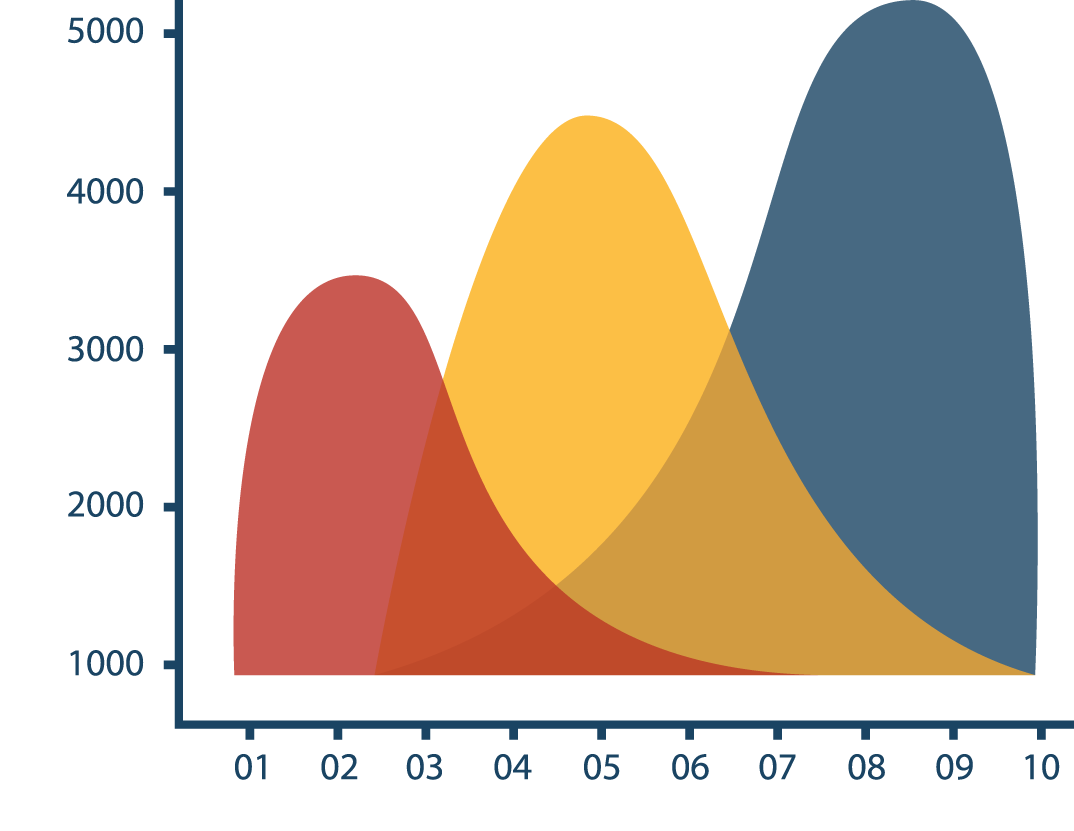
\includegraphics[width=0.5cm]{Figures/Graph.png} next to the PDF (top) panel or the CDF (bottom) panel to view the fits. If the Box--Cox transformation was selected, the graphs show the transformed elemental contents fitted with a Gaussian distribution. Otherwise, the graphs show both normal and log-normal fits to the raw data (Fig.~\ref{fig:DF-results}); the samples are the black points. A constituent with zero or negative values (such as $\delta^{13}$C) cannot be fitted with a log-normal distribution; for it, check \textit{Box-cox transformation} (which leaves it untransformed) to see the normal fit.

\begin{figure}[ht]
    \centering
    \begin{tabular}{cc}
        a) & b) \\
        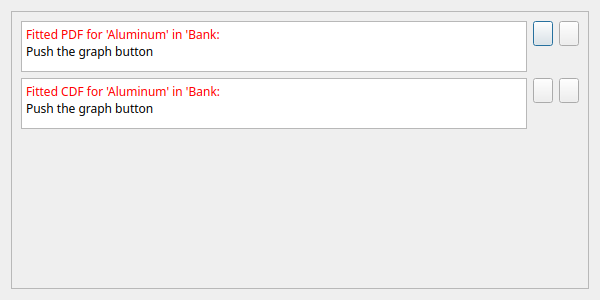
\includegraphics[width=0.46\textwidth]{Figures/DF_result_window.png} &
        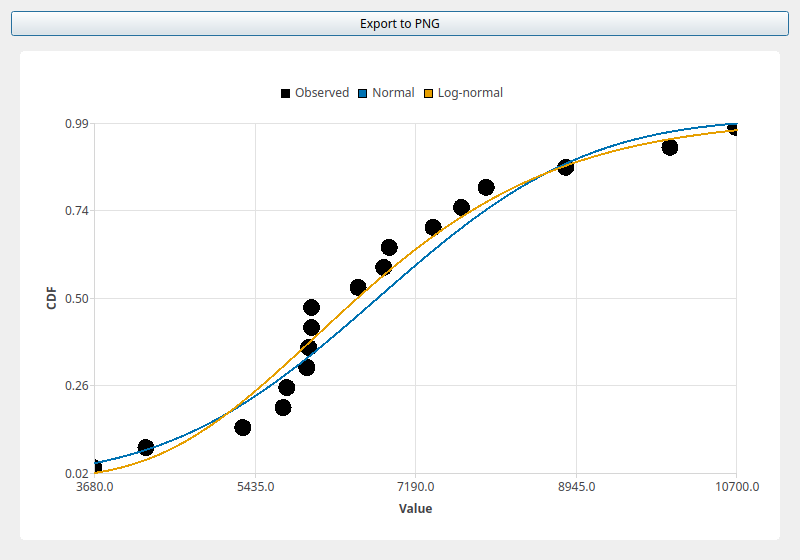
\includegraphics[width=0.46\textwidth]{Figures/DF_graph.png}
    \end{tabular}
    \caption{Distribution fitting without Box--Cox transformation: a) results window, b) CDF graph showing the empirical distribution with fitted normal and log-normal curves.}
    \label{fig:DF-results}
\end{figure}
\FloatBarrier

\begin{figure}[ht]
    \centering
    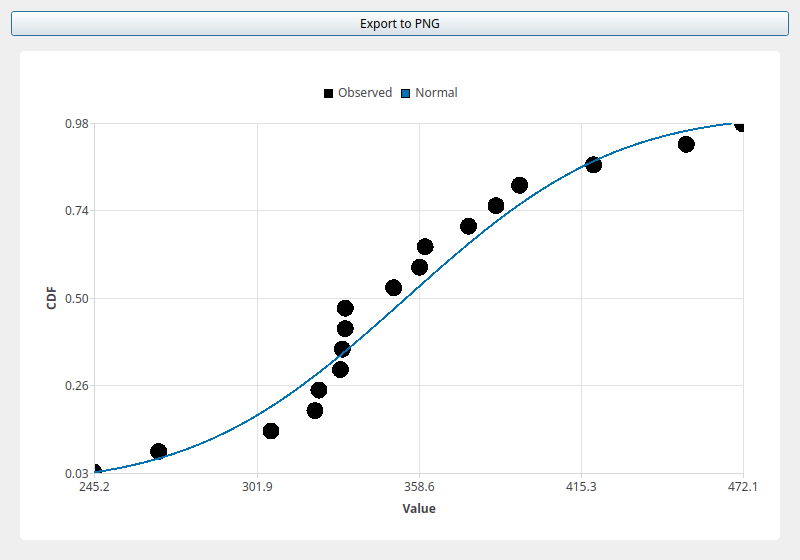
\includegraphics[width=0.46\textwidth]{Figures/DF_graph_BoxCox.png}
    \caption{Distribution fitting with Box--Cox transformation, showing the transformed data fitted with a Gaussian distribution.}
    \label{fig:DF_results_BoxCox}
\end{figure}
\FloatBarrier

\subsection{Kolmogorov--Smirnov for individual group/element}\label{sec:ks-individual}
The Kolmogorov--Smirnov (K--S) tool lets you visually inspect the normality of an element's distribution within a source group. The K--S test assesses normality based on the maximum difference between the empirical distribution function (EDF) of the sample and the cumulative distribution function (CDF) of a specified theoretical distribution (either normal or log-normal).

To perform the K--S test, select \textbf{Tools}$\rightarrow$\textbf{Other Statistical Tools}$\rightarrow$\textbf{Data exploration}$\rightarrow$\textbf{Kolmogorov--Smirnov for individual group/element}. In the central form, choose the element, the source group, and the theoretical distribution (normal or log-normal) against which to test. Click \textbf{Ok}.

In the results window, click the graph button~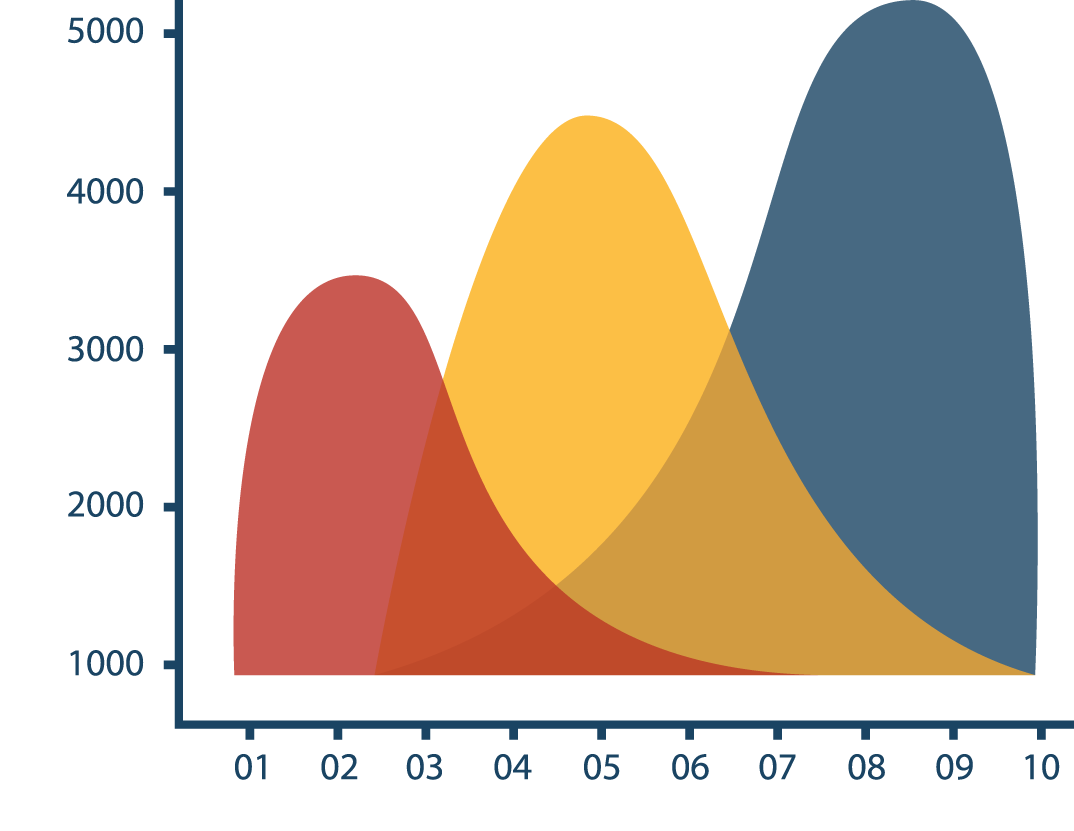
\includegraphics[width=0.5cm]{Figures/Graph.png} to view the empirical distribution, the fitted theoretical distribution, and the difference between them (Fig.~\ref{fig:K-S-test}). The magnitude of the maximum difference between the empirical and theoretical CDFs indicates how well the chosen distribution represents the element's data: a smaller difference indicates a better fit. A constituent with zero or negative values (such as $\delta^{13}$C) cannot be compared with a log-normal distribution; the tool then stops with a message.

\begin{figure}[ht]
    \centering
    \begin{tabular}{cc}
        a) & b) \\
        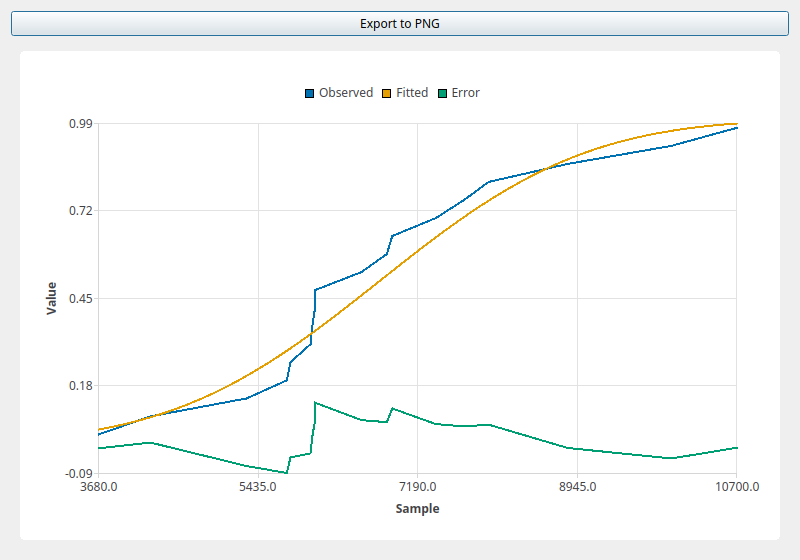
\includegraphics[width=0.46\textwidth]{Figures/K-S-normal.png} &
        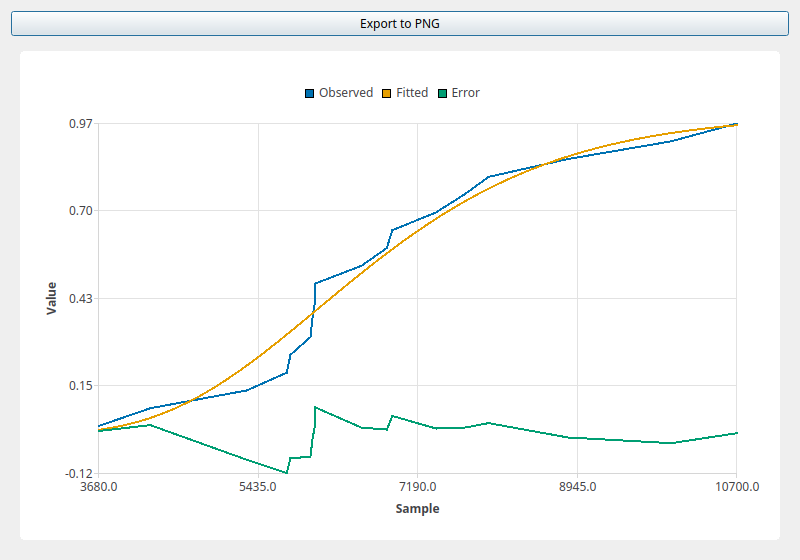
\includegraphics[width=0.46\textwidth]{Figures/K-S-Lognormal.png}
    \end{tabular}
    \caption{K--S test for an element fitted with a) a normal distribution and b) a log-normal distribution.}
    \label{fig:K-S-test}
\end{figure}
\FloatBarrier

\subsection{Kolmogorov--Smirnov for a group}\label{sec:tool-ks}
The Kolmogorov--Smirnov test for a group runs the K--S analysis on every element in a specified source group and reports the maximum difference between the empirical and theoretical CDFs for each element.

To use this tool, select \textbf{Tools}$\rightarrow$\textbf{Other Statistical Tools}$\rightarrow$\textbf{Data exploration}$\rightarrow$\textbf{Kolmogorov--Smirnov for a group}. In the central form, choose the source group and the theoretical distribution (normal or log-normal), then click \textbf{Ok}.

In the result window, click the table button~
\includegraphics[width=0.5cm]{Figures/table.png} to view the maximum CDF differences in tabular form, or the graph button~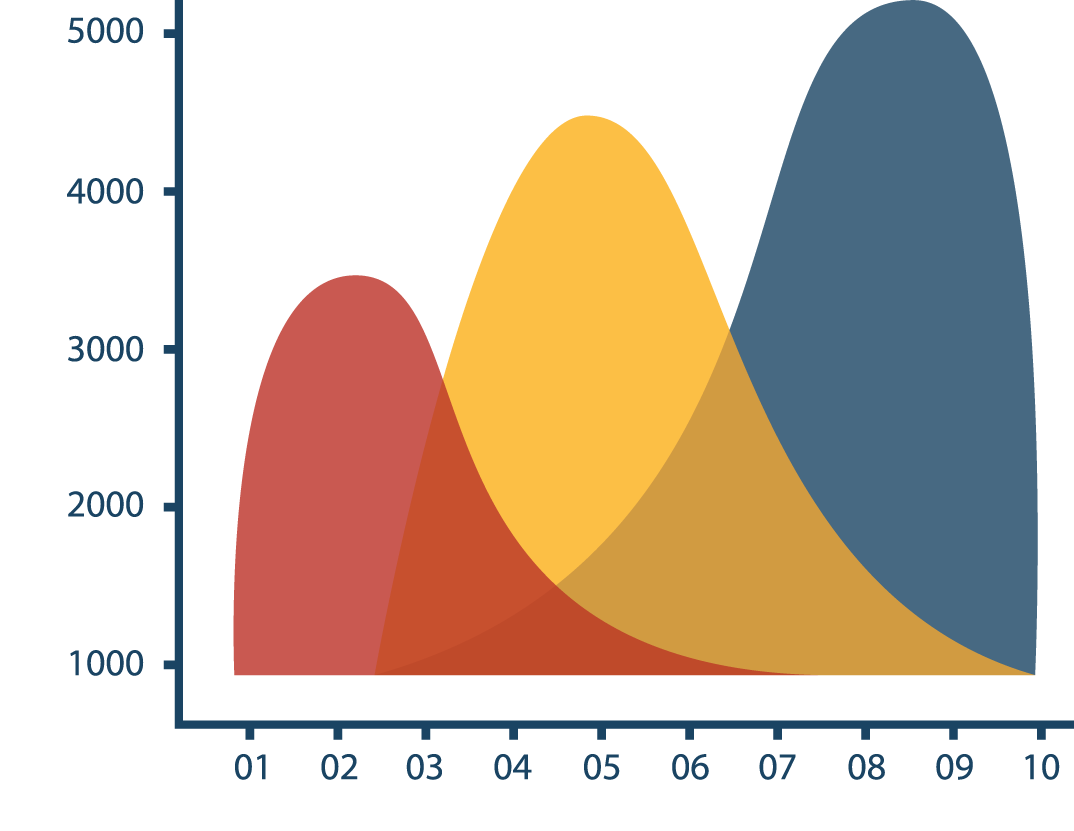
\includegraphics[width=0.5cm]{Figures/Graph.png} to view them as a bar chart (Fig.~\ref{fig:K-S-results-group}).

\begin{figure}[ht]
    \centering
    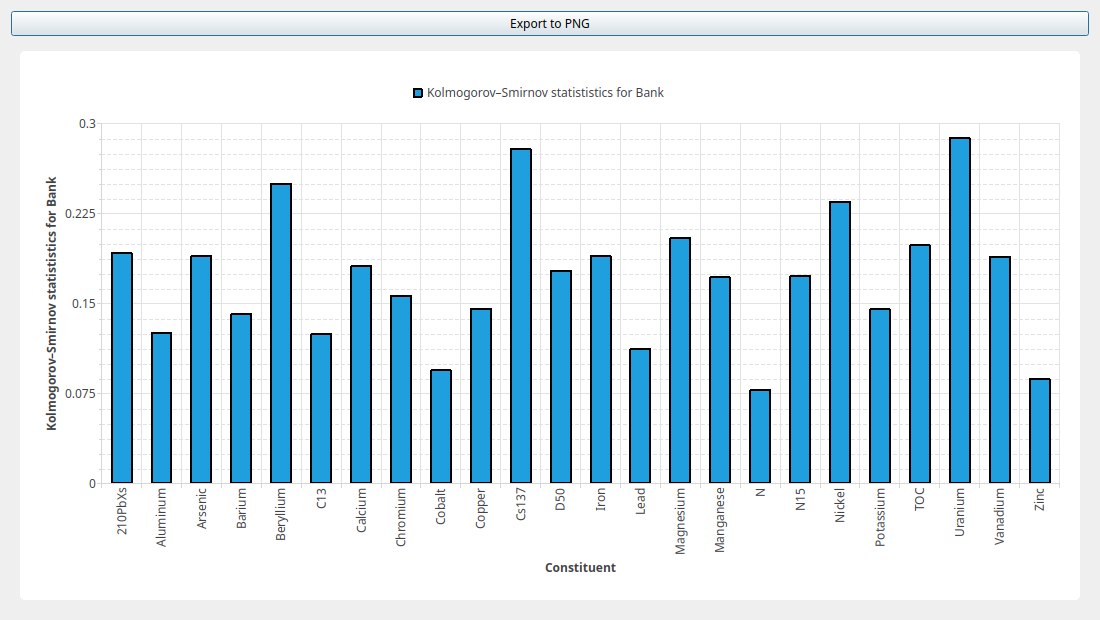
\includegraphics[width=\textwidth]{Figures/K-S-group-Normal.png}
    \caption{K--S test results for all elements in a source group.}
    \label{fig:K-S-results-group}
\end{figure}
\FloatBarrier

\subsection{Optimal Box-Cox parameters}\label{sec:tool-boxcox}
The optimal Box--Cox parameters tool determines the value of $\lambda$ that transforms the elemental content of a specified source group to most closely resemble a normal distribution. The Box--Cox transformation is defined as:
\begin{equation}
    \hat{y}_{i,j,k} = \begin{cases}
        \dfrac{\left(\dfrac{y_{i,j,k}}{\sigma_{i,j}}\right)^{\lambda} - 1}{\lambda} & \text{for } \lambda \neq 0 \\[1.5em]
        \log\left(\dfrac{y_{i,j,k}}{\sigma_{i,j}}\right) & \text{for } \lambda = 0
    \end{cases}
\end{equation}

The optimization minimizes the maximum difference between the CDF of the transformed data and a fitted normal distribution, as measured by the Kolmogorov--Smirnov statistic. A value of $\lambda$ close to 1 indicates that the data are already well represented by a normal distribution; a value close to 0 indicates that the data more closely follow a log-normal distribution.

To compute the optimal Box--Cox parameters, select \textbf{Tools}$\rightarrow$\textbf{Other Statistical Tools}$\rightarrow$\textbf{Data exploration}$\rightarrow$\textbf{Optimal Box-Cox parameters}. In the central form, choose the source group to analyze and click \textbf{Ok}.

The result window contains the optimal $\lambda$ for every element in the specified source group. Click the table button~
\includegraphics[width=0.5cm]{Figures/table.png} to view the values in tabular form, or the graph button to plot them as bars; the zero line of the plot separates positive from negative $\lambda$. A constituent with zero or negative values is not transformed, and its $\lambda$ is shown as 1; the program lists these constituents.
\section{Element selection}\label{sec:tools-selection}
\subsection{Analysis of Variance for element selection}\label{sec:tool-anova}
Analysis of variance (ANOVA) helps evaluate how effectively each element distinguishes between source groups by comparing the variation in elemental content between groups against the variation within groups. Elements that show large between-group differences relative to within-group variability are good candidates for fingerprinting.

One-way ANOVA is a statistical technique used to compare the means of three or more samples (assuming equal variances) to determine whether at least one sample mean differs significantly from the others. The F-statistic is the ratio of between-group variance to within-group variance:
\begin{equation}
    F = \frac{MS_{\mathrm{between}}}{MS_{\mathrm{within}}}
\end{equation}
where $MS_{\mathrm{between}}$ (mean square between) is the variance between groups and $MS_{\mathrm{within}}$ (mean square within) is the variance within groups.

The mean squares are calculated as:
\begin{equation}
    MS_{\mathrm{between}} = \frac{SS_{\mathrm{between}}}{df_{\mathrm{between}}}, \qquad MS_{\mathrm{within}} = \frac{SS_{\mathrm{within}}}{df_{\mathrm{within}}}
\end{equation}
where $SS_{\mathrm{between}}$ and $SS_{\mathrm{within}}$ are the sums of squares between and within groups, $df_{\mathrm{between}} = n - 1$ is the degrees of freedom between groups (with $n$ the number of groups), and $df_{\mathrm{within}} = l - n$ is the degrees of freedom within groups (with $l$ the total number of observations).

The sums of squares are calculated as:
\begin{equation}
    SS_{\mathrm{between}} = \sum_{i=1}^{n} n_i (\bar{y}_i - \bar{y})^2
\end{equation}
\begin{equation}
    SS_{\mathrm{within}} = \sum_{i=1}^{n} \sum_{k=1}^{n_i} (y_{i,k} - \bar{y}_i)^2
\end{equation}
where $n_i$ is the number of observations in group $i$, $\bar{y}_i$ is the mean of group $i$, $\bar{y}$ is the overall mean across all observations, and $y_{i,k}$ is the $k$th observation in group $i$.

The resulting $F$ value is converted to a p-value:
\begin{equation}
    p = 1 - \Xi(F;\, n - 1,\, l - n)
\end{equation}
where $\Xi$ is the cumulative distribution function of the $F$ distribution with $n - 1$ and $l - n$ degrees of freedom.

To perform ANOVA, select \textbf{Tools}$\rightarrow$\textbf{Other Statistical Tools}$\rightarrow$\textbf{Element selection}$\rightarrow$\textbf{Analysis of Variance for element selection}. You can run the analysis on raw elemental contents, log-transformed contents, or Box--Cox transformed contents. To use source elemental profiles adjusted for size, organic matter, or both, select the target sample on which the correction should be based. Selecting \textit{Modify the included elements based on the results} automatically excludes elements whose p-value exceeds the specified \textbf{P-value threshold}; this threshold identifies elements with low discriminating power. Click \textbf{Ok} to run the analysis.

When the analysis is complete, click the graph button~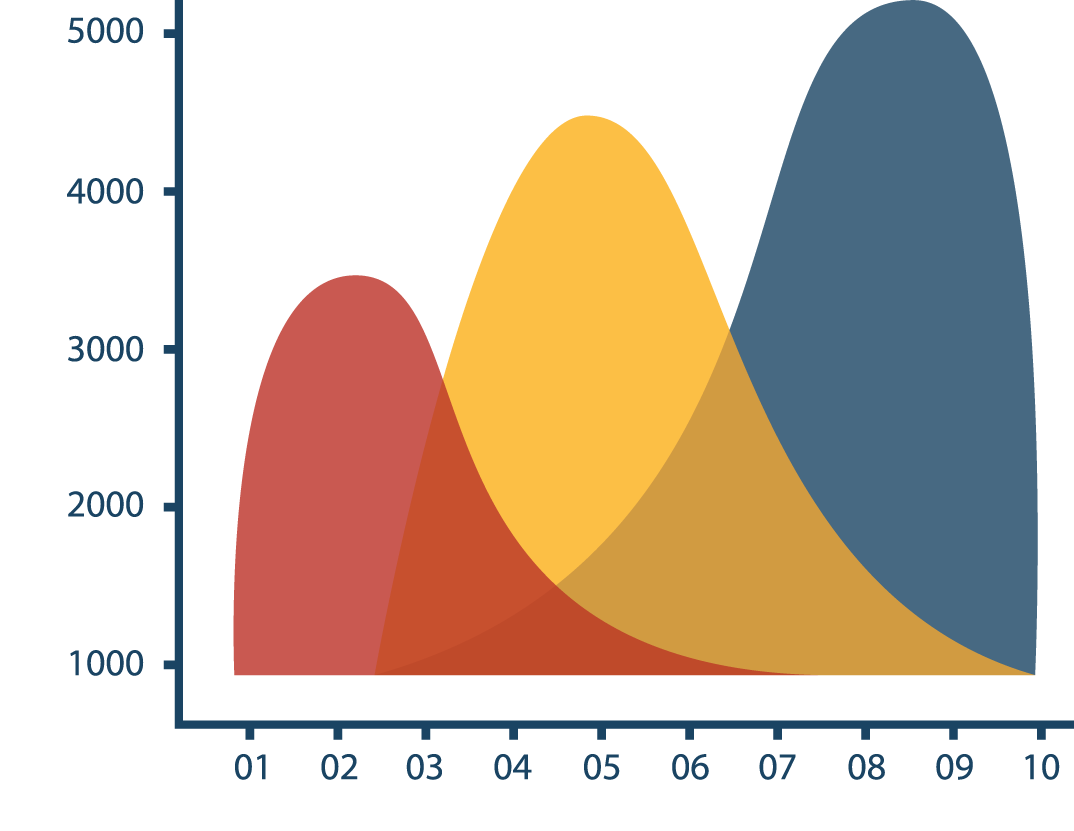
\includegraphics[width=0.5cm]{Figures/Graph.png} to view the p-values for each element graphically, or the table button~
\includegraphics[width=0.5cm]{Figures/table.png} to view them in tabular form. For example, Fig.~\ref{fig:Anova_Results} shows that Arsenic and Cobalt have low discriminating power in the uncorrected example data (p-values of about 0.13 and 0.12).

\begin{tcolorbox}[colback=yellow!10,colframe=yellow!50!black,title=Note]
The discriminating power of a tracer depends on the data it is computed from. After the organic matter and size correction, a tracer can gain or lose discriminating power: in the example, with the power-law correction for target sample CTAIL1, the ANOVA p-value of Cobalt falls from about 0.12 to about $10^{-9}$. Before removing a tracer, evaluate it on the data you will use for fingerprinting (corrected or not), and compare the results of several tools (ANOVA, discriminant power, stepwise DFA) rather than relying on one.
\end{tcolorbox}

\begin{figure}[ht]
    \centering
    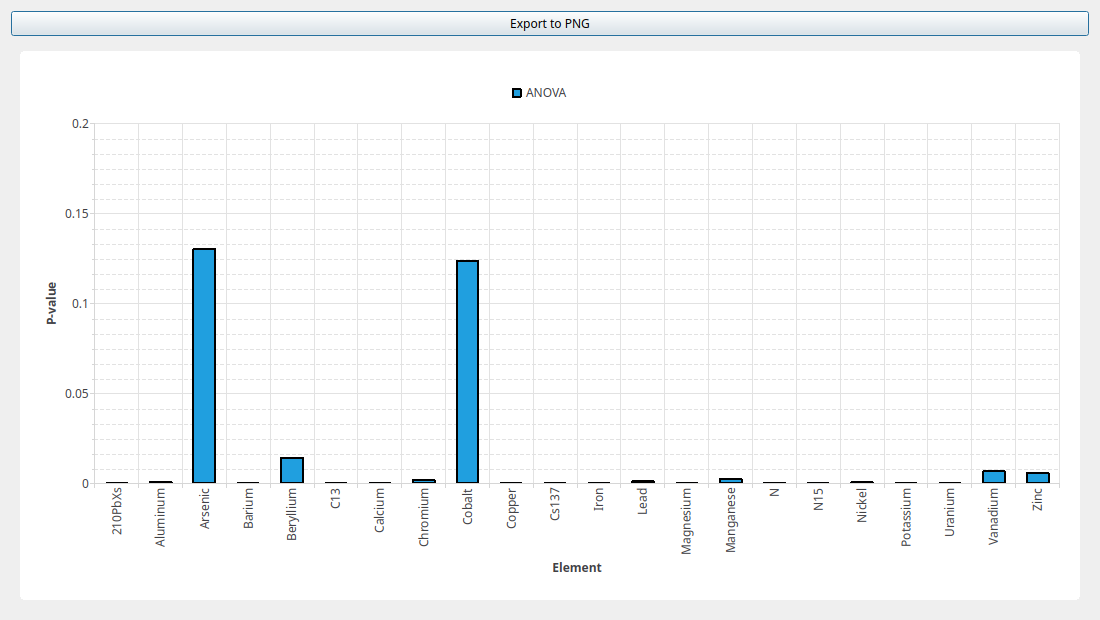
\includegraphics[width=\textwidth]{Figures/ANOVA_results.png}
    \caption{Results of the ANOVA analysis.}
    \label{fig:Anova_Results}
\end{figure}
\FloatBarrier

\subsection{Auto-select elements}\label{sec:tool-autoselect}
The auto-select tool identifies a small set of elements that effectively distinguishes between all pairs of source groups. For each pair of source groups, it performs a t-test on each element and then selects a predetermined number of elements with the lowest p-values from each pair.

To use this tool, select \textbf{Tools}$\rightarrow$\textbf{Other Statistical Tools}$\rightarrow$\textbf{Element selection}$\rightarrow$\textbf{Auto-select elements}. In the form that appears, you can choose whether to include isotopes in the analysis and whether to adjust the source elemental profiles based on size and organic matter. To apply the selection automatically to the constituent inclusion list, check \textit{Modify the included elements based on the results}. The \textbf{Number of elements from each pair} field sets how many of the lowest-p-value elements are selected from each pair of source groups; a larger number yields a larger total selection. Click \textbf{Ok} to run the analysis.

The result window contains two panels. The first panel shows the p-value for each element from the t-test on each pair of source groups (Fig.~\ref{fig:autoselect-p-vals}). The second panel lists the selected elements with the smallest p-value that selected each (Fig.~\ref{fig:autoselect-results}); in the example, Calcium, Copper, Cs137, Iron, Magnesium, N, Potassium and Uranium. Particle size and organic matter constituents (D50, TOC) are never tested or selected.

\begin{figure}[ht]
    \centering
    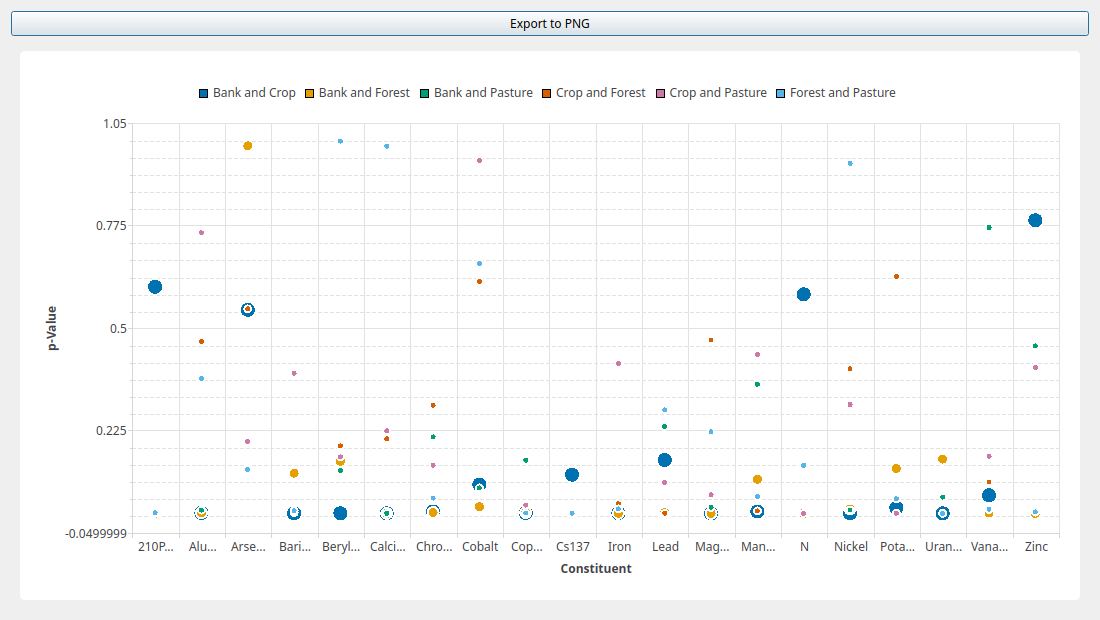
\includegraphics[width=\textwidth]{Figures/Auto-Select-p-value.png}
    \caption{Pairwise t-test p-values for auto-selection of elements.}
    \label{fig:autoselect-p-vals}
\end{figure}
\FloatBarrier

\begin{figure}[ht]
    \centering
    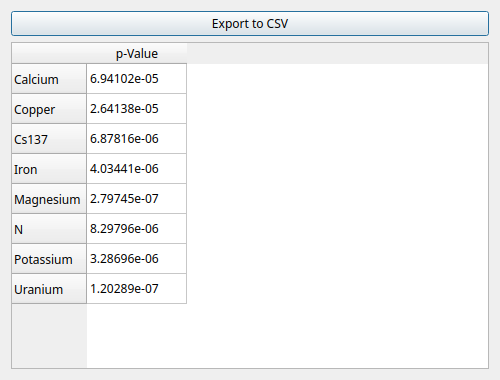
\includegraphics[width=0.46\textwidth]{Figures/Autoselect-selectedelements.png}
    \caption{Elements selected by the auto-select tool.}
    \label{fig:autoselect-results}
\end{figure}
\FloatBarrier

\subsection{Elements' discriminant power (Two-way)}\label{sec:tool-edp}
This tool, \textbf{Tools}$\rightarrow$\textbf{Other Statistical Tools}$\rightarrow$\textbf{Element selection}$\rightarrow$\textbf{Elements' discriminant power (Two-way)}, functions like the multi-way version described in Section~\ref{sec:edpm}, except that the analysis is performed between two specific source groups that you choose, rather than across all pairs.

\subsection{Elements' discriminant power (Multi-way)}\label{sec:edpm}
The Elements' Discriminant Power (Multi-way) tool evaluates each element's ability to distinguish between every pair of source groups. It produces three types of results for each element and source pair:

\begin{enumerate}
    \item The ratio of the between-group mean distance to the within-group standard deviation.
    \item The \textit{discriminant fraction}: the proportion of samples that can be correctly assigned to one of the two source groups based on that single element alone.
    \item A t-test p-value for the null hypothesis that the mean elemental content is the same in the two source groups.
\end{enumerate}

To run the multi-way discriminant power analysis, select \textbf{Tools}$\rightarrow$\textbf{Other Statistical Tools}$\rightarrow$\textbf{Element selection}$\rightarrow$\textbf{Elements' discriminant power (Multi-way)}. In the central form:

\begin{itemize}
    \item Choose whether to run the analysis on untransformed or Box--Cox transformed elemental contents.
    \item Check \textit{Include target samples} to add the target samples as one more group. The pairs then include the target group with each source group, which shows which constituents make the target samples unlike a source. A constituent that separates the target from every source is one that no mixture of the sources can reproduce, a warning similar to a failed bracket test.
    \item Set the \textbf{p-value threshold} to determine the cutoff above which values are highlighted in the resulting table.
    \item To run the analysis on data corrected for size and organic matter, select the target sample on which the correction should be based. To run on uncorrected data, leave the \textit{OM and Size corrected based on target sample} field blank.
\end{itemize}

Click \textbf{Ok}.

The result window contains three panels. The first panel reports the ratio of the between-group mean distance to the within-group standard deviation for every pair of source groups. Click the table button~
\includegraphics[width=0.5cm]{Figures/table.png} next to the panel to view the values in tabular form. A higher value indicates greater discriminating power between the corresponding pair of source groups.

The second panel reports the discriminant fraction for each element and source pair. Click the table button~
\includegraphics[width=0.5cm]{Figures/table.png} next to the panel to view the values. A discriminant fraction of 0.5 means that samples with a given elemental content are equally likely to belong to either source group, indicating no discriminating power; values closer to 1 indicate stronger discriminating power.

\begin{figure}[ht]
    \centering
    \begin{tabular}{cc}
        a) & b) \\
        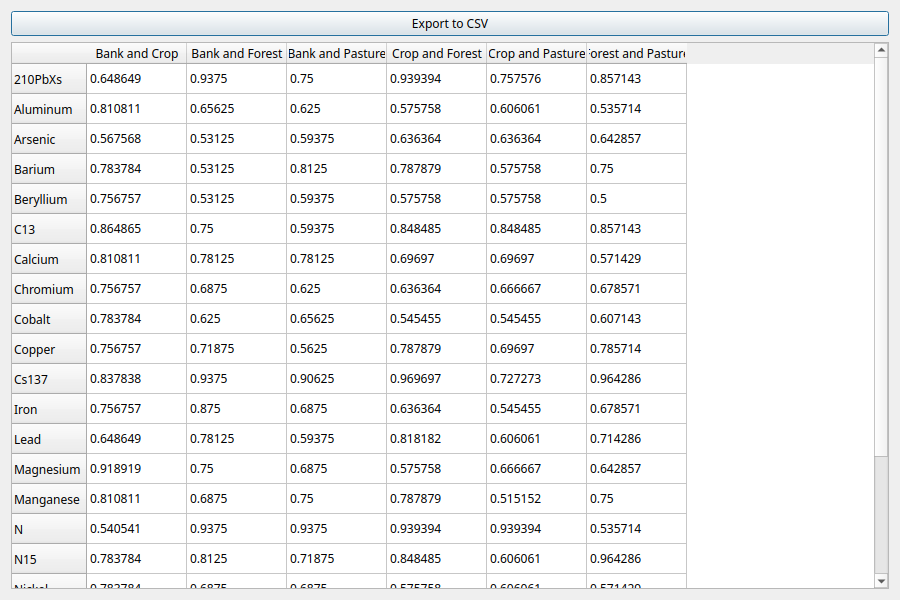
\includegraphics[width=0.46\textwidth]{Figures/Discriminant_Fraction.png} &
        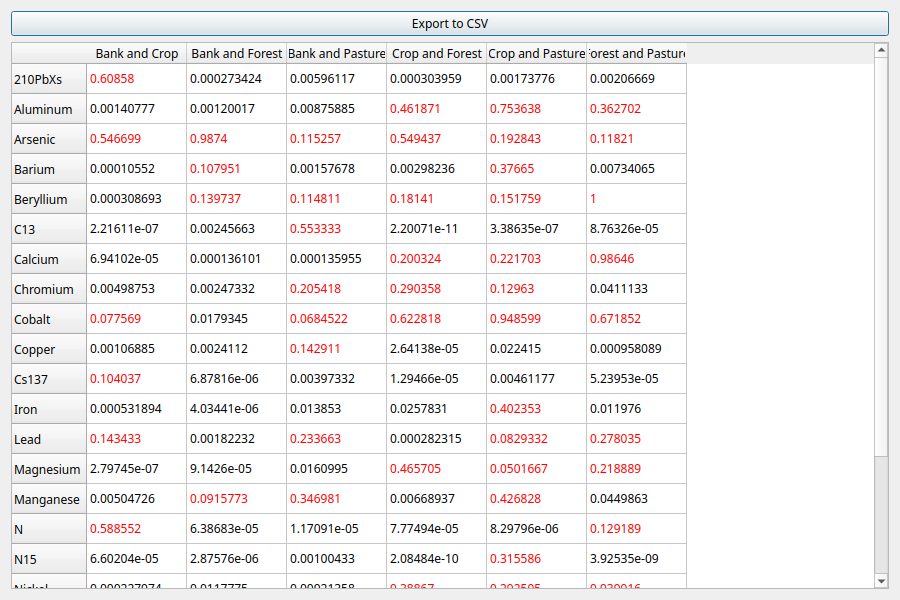
\includegraphics[width=0.46\textwidth]{Figures/Discriminant_p_value.png}
    \end{tabular}
    \caption{a) Discriminant fraction for each element and source-group pair. b) Discriminant t-test p-value for each element and source-group pair.}
    \label{fig:discriminant-power-multiway}
\end{figure}
\FloatBarrier

The third panel reports the t-test p-value for each element and source pair. Click the table button~
\includegraphics[width=0.5cm]{Figures/table.png} next to the panel to view the values. Entries highlighted in red indicate that the element lacks significant discriminating power between the corresponding pair of source groups (i.e., the p-value exceeds the threshold).
\section{Discriminant function analysis}\label{sec:dfa-tools}
Each discriminant function analysis tool comes in two versions: the plain one uses all the constituents given to it (normally with \textit{Use only selected elements} checked), and the stepwise one selects constituents by forward selection (Section~\ref{sec:dfa-theory}). Step~4 of the fingerprinting menus is the stepwise multi-way version.

\subsection{Discriminant function analysis (one vs.\ one)}\label{sec:tool-dfa}
The one-vs.-one DFA performs discriminant function analysis between two source groups that you choose. The first step in any DFA is to determine which elements to include by evaluating the $\chi^2$ statistic and Wilks' Lambda. The stepwise DFA begins with the element that provides the highest discriminating power between the two sources and then adds elements one by one, at each step selecting the element that maximizes the discriminating power.

To perform a stepwise one-vs.-one DFA, choose \textbf{Tools}$\rightarrow$\textbf{Other Statistical Tools}$\rightarrow$\textbf{Discriminant function analysis}$\rightarrow$\textbf{Stepwise discriminant function analysis (one vs.\ one)} from the tools window. In the central form, specify the two source groups for which the DFA is to be performed. Check \textit{Box-Cox transformation} to perform the DFA on data transformed using the optimal $\lambda$ for normality. Click \textbf{Ok}.

The result window contains three panels, each listing the constituents in the order in which they were added. The first panel contains the $\chi^2$ p-value after each addition. Click the table button~
\includegraphics[width=0.5cm]{Figures/table.png} to view the values in tabular form, or the graph button~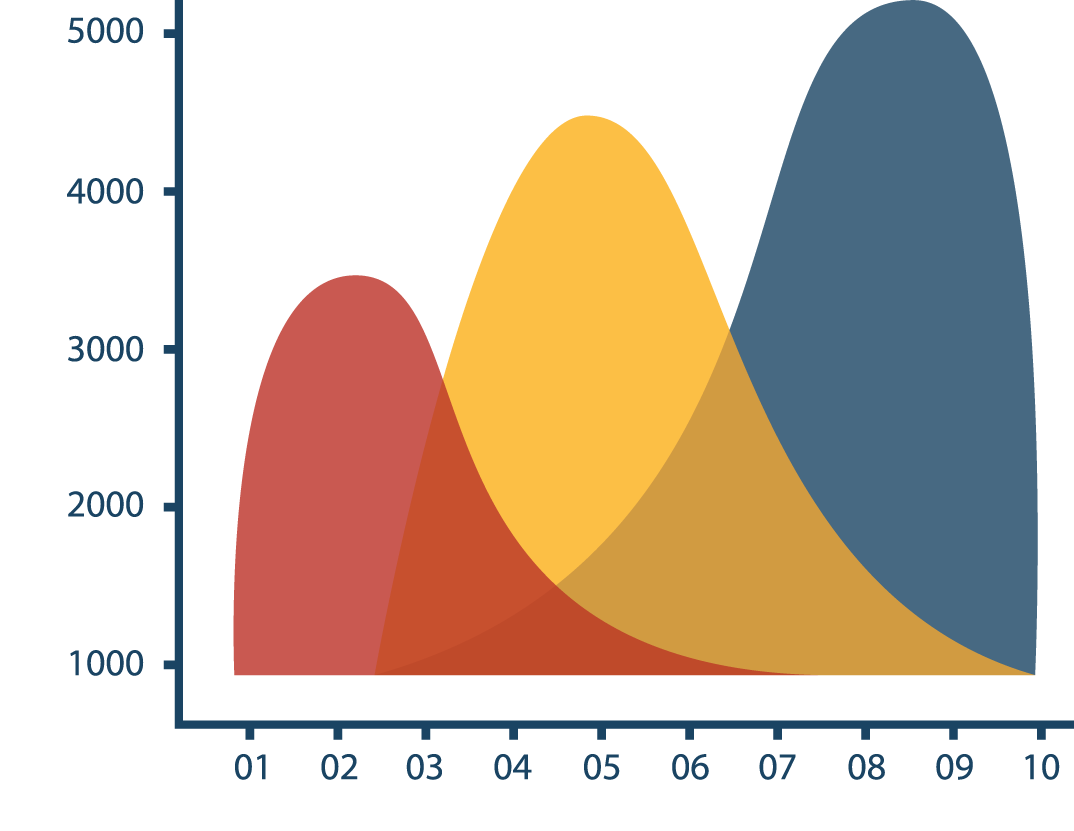
\includegraphics[width=0.5cm]{Figures/Graph.png} to view them graphically.

For example, for Bank and Crop in the example data, Fig.~\ref{fig:two-way-DFA-analysis} shows that Magnesium has the highest discriminating power on its own, and that the constituents added after Copper do not increase the discriminating power between the two groups. Note that an element with low discriminating power between one pair of groups may still discriminate effectively between other pairs.

\begin{figure}[ht]
    \centering
    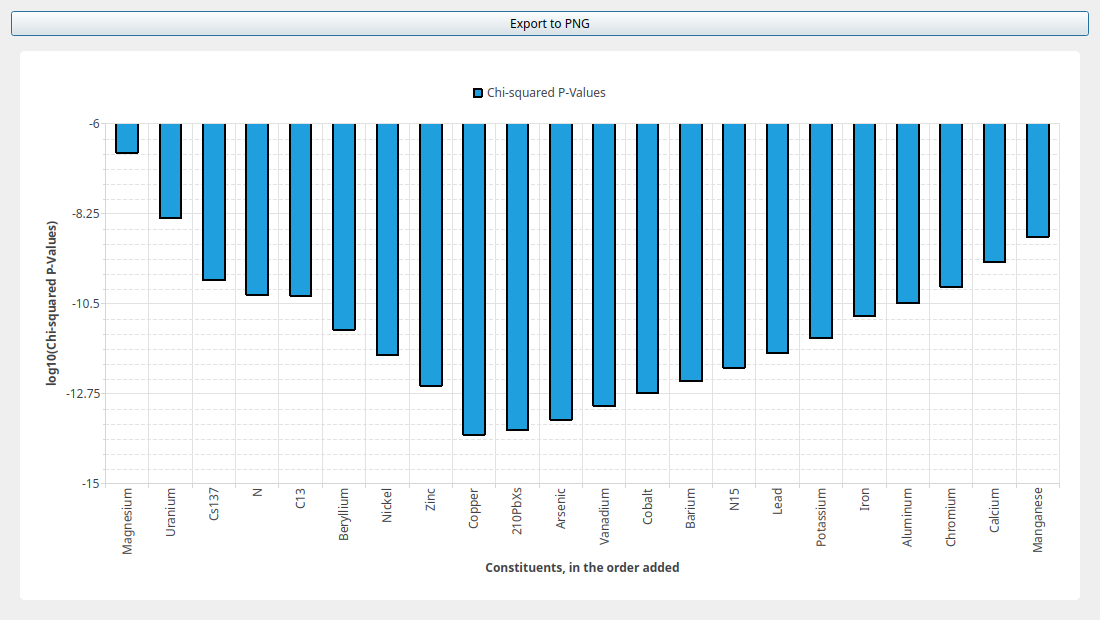
\includegraphics[width=\textwidth]{Figures/Chi2p-value-stepwise-twoway-DFA.png}
    \caption{Base-10 logarithm of the $\chi^2$ p-value after each constituent is added, for stepwise one-vs.-one DFA between Bank and Crop.}
    \label{fig:two-way-DFA-analysis}
\end{figure}
\FloatBarrier

The $\chi^2$ p-value decreases as constituents are added up to Copper (nine constituents: Magnesium, Uranium, Cs137, N, C13, Beryllium, Nickel, Zinc and Copper), then rises as additional constituents are included.

The second panel shows Wilks' $\Lambda$ as a function of the number of elements included (Fig.~\ref{fig:two-way-wilks-lambda}).

\begin{figure}[ht]
    \centering
    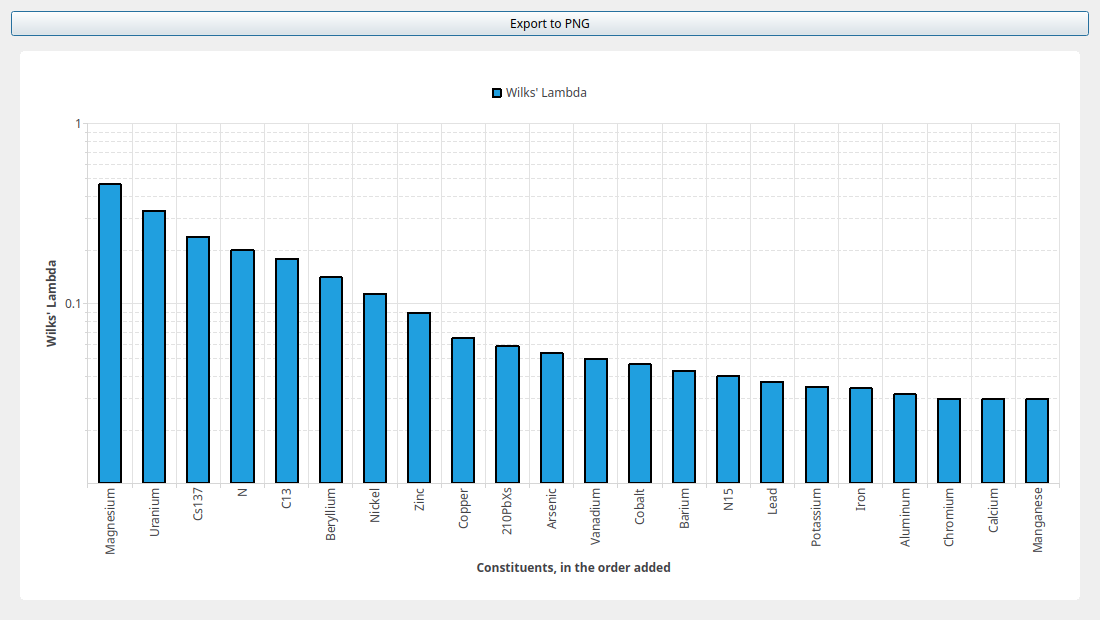
\includegraphics[width=\textwidth]{Figures/Wilks-Lambda-stepwise-twoway-DFA.png}
    \caption{Wilks' $\Lambda$ values as elements are added successively in two-way DFA.}
    \label{fig:two-way-wilks-lambda}
\end{figure}
\FloatBarrier

Wilks' $\Lambda$ decreases with every constituent added, which is why the selection is based on the p-value.

The third panel shows the p-value for the F-test on the discriminant scores obtained from the two source groups (Fig.~\ref{fig:two-way-F-test-P-value}).

\begin{figure}[ht]
    \centering
    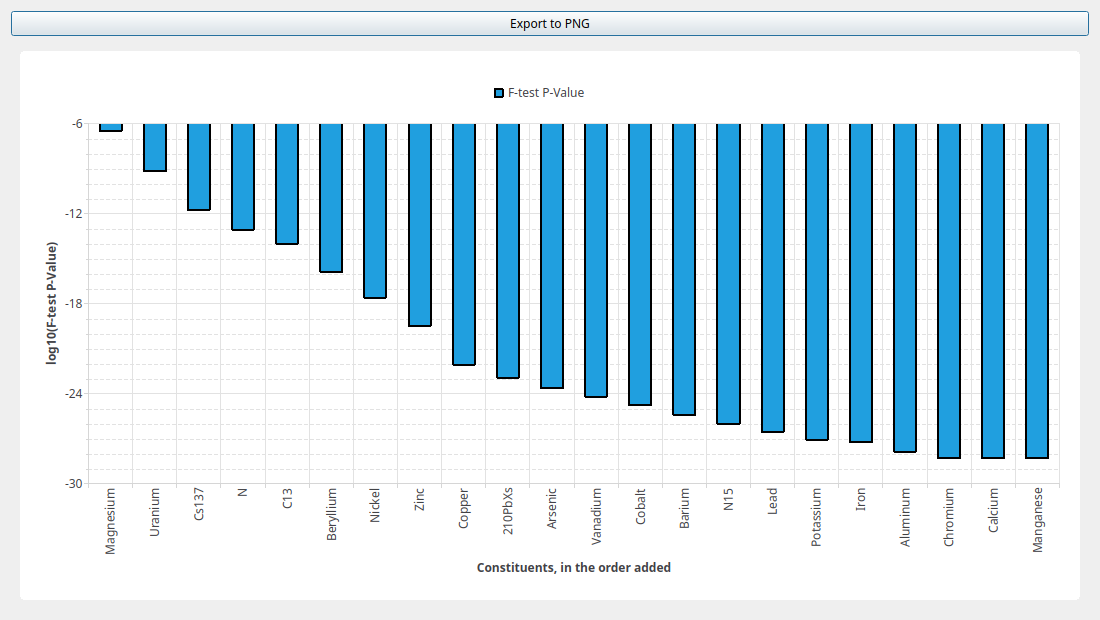
\includegraphics[width=\textwidth]{Figures/F-test_P_value_two_way_DFA.png}
    \caption{Base-10 logarithm of the F-test p-value after each constituent is added, for stepwise one-vs.-one DFA between Bank and Crop.}
    \label{fig:two-way-F-test-P-value}
\end{figure}
\FloatBarrier

To view the separation produced by a chosen set of elements, first select the elements to include via \textbf{Settings}$\rightarrow$\textbf{Constituent Properties} (the stepwise DFA results can guide this choice). Then choose \textbf{Tools}$\rightarrow$\textbf{Other Statistical Tools}$\rightarrow$\textbf{Discriminant function analysis}$\rightarrow$\textbf{Discriminant function analysis (one vs.\ one)}. Select the two source groups, choose whether to apply the OM and size correction and the Box--Cox transformation, and check \textit{Use only selected elements} so that only the elements marked for inclusion are considered. The result window contains the $\chi^2$ p-value, the F-test p-value, and the calculated discriminant scores for the two source groups. Click the graph button~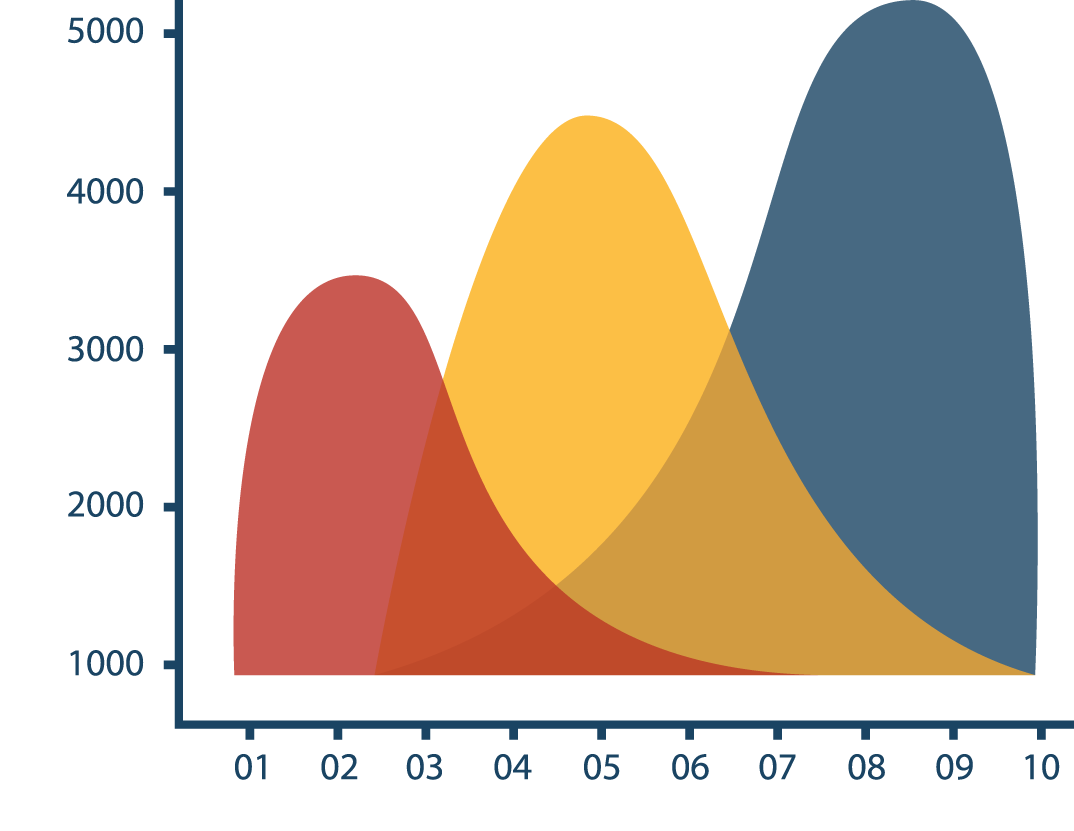
\includegraphics[width=0.5cm]{Figures/Graph.png} on the side of the \textbf{Projected Elemental Profiles} panel to view the discriminant scores for the samples in each source group (Fig.~\ref{fig:two-way-DFA-scatter}).

\begin{figure}[ht]
    \centering
    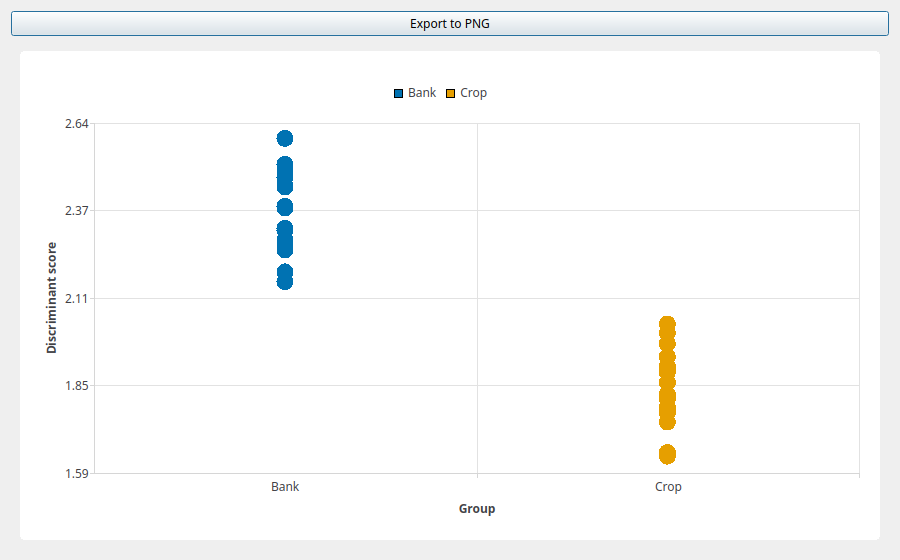
\includegraphics[width=\textwidth]{Figures/DFA_Scatter_2way.png}
    \caption{Discriminant scores of the samples in source groups Bank and Crop, with the seven constituents selected in step~4 included.}
    \label{fig:two-way-DFA-scatter}
\end{figure}
\FloatBarrier

\subsection{Discriminant function analysis (Multi-way)}\label{sec:tool-dfam}
This tool performs discriminant function analysis among all source groups at once, without stepwise selection: it uses all the constituents given to it. Run it with \textit{Use only selected elements} checked after step~4 (Section~\ref{sec:multiway-dfa}) to see the separation achieved by the selected constituents. It reports, for each source group, the $\chi^2$ and F-test p-values of its separation from the rest of the samples (Fig.~\ref{fig:Chi2-DFA-multiway-for-selected-elements}), the discriminant scores and the eigenvectors. Choose \textbf{Tools}$\rightarrow$\textbf{Other Statistical Tools}$\rightarrow$\textbf{Discriminant function analysis}$\rightarrow$\textbf{Discriminant function analysis (Multi-way)}; the stepwise version, \textbf{Stepwise discriminant function analysis (Multi-way)}, is step~4 of the fingerprinting menus.

\subsection{Discriminant function analysis (one vs.\ the rest)}\label{sec:tool-dfaonevsrest}
The one-vs-the-rest DFA performs discriminant function analysis between all samples belonging to one specified source group and all other samples taken together. To perform a stepwise one-vs-the-rest DFA, choose \textbf{Tools}$\rightarrow$\textbf{Other Statistical Tools}$\rightarrow$\textbf{Discriminant function analysis}$\rightarrow$\textbf{Stepwise discriminant function analysis (one vs.\ the rest)} from the tools panel. In the central form, select the source group to be tested against all others, and choose whether to apply the Box--Cox transformation and the organic matter and size correction. Click \textbf{Ok}.

The results are analogous to those of the one-vs.-one stepwise DFA, except that the statistics are calculated between the chosen source group and the pooled remainder of the samples. Figure~\ref{fig:Chi2-DFA-onevsrest} shows the $\chi^2$ p-values for the Bank source group versus the rest of the samples: Calcium separates Bank best on its own, and the p-value is smallest after Beryllium, the eleventh constituent added.

\begin{figure}[ht]
    \centering
    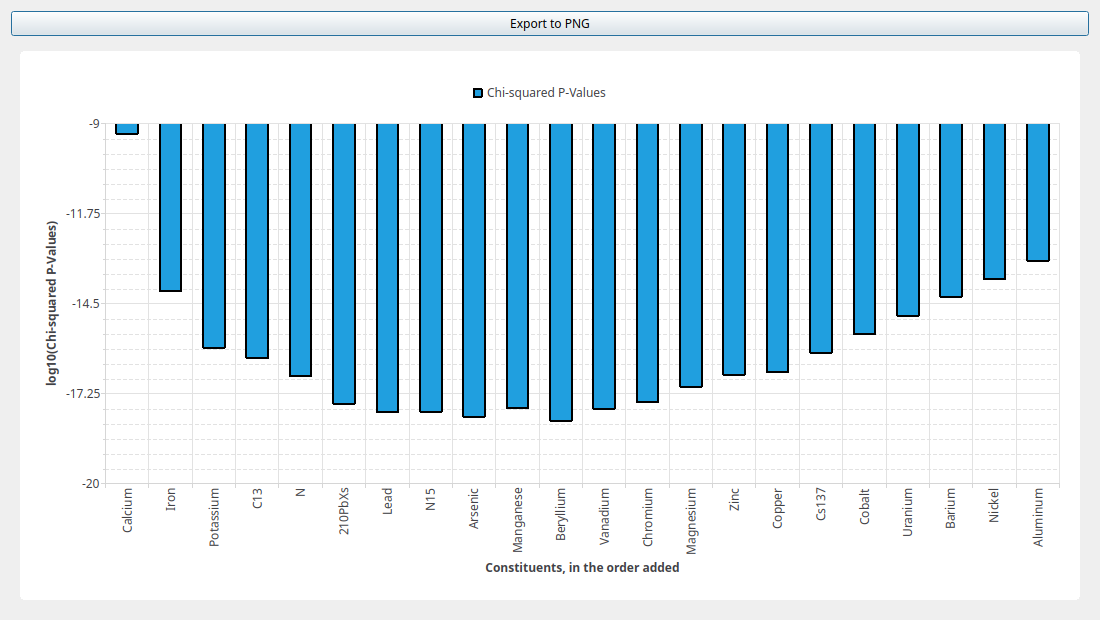
\includegraphics[width=\textwidth]{Figures/Chi2p-value-stepwise-onevstherest-DFA.png}
    \caption{Base-10 logarithm of the $\chi^2$ p-value after each constituent is added, for stepwise one-vs-the-rest DFA between Bank and the other sources.}
    \label{fig:Chi2-DFA-onevsrest}
\end{figure}
\FloatBarrier

After running the stepwise DFA, you can use the results to choose which elements to include in subsequent fingerprinting analyses. To do so, go to \textbf{Settings}$\rightarrow$\textbf{Constituent Properties} and use the \textbf{Include in analysis} column to mark each constituent as included or excluded.

To visualize the separation produced by a chosen set of elements, choose \textbf{Tools}$\rightarrow$\textbf{Other Statistical Tools}$\rightarrow$\textbf{Discriminant function analysis}$\rightarrow$\textbf{Discriminant function analysis (one vs.\ the rest)}. Select the source group to be tested, choose whether to apply the OM and size correction and the Box--Cox transformation, and check \textit{Use only selected elements} so that only the included elements are considered. The result window contains the $\chi^2$ p-value, the F-test p-value, and the calculated discriminant scores. Click the graph button~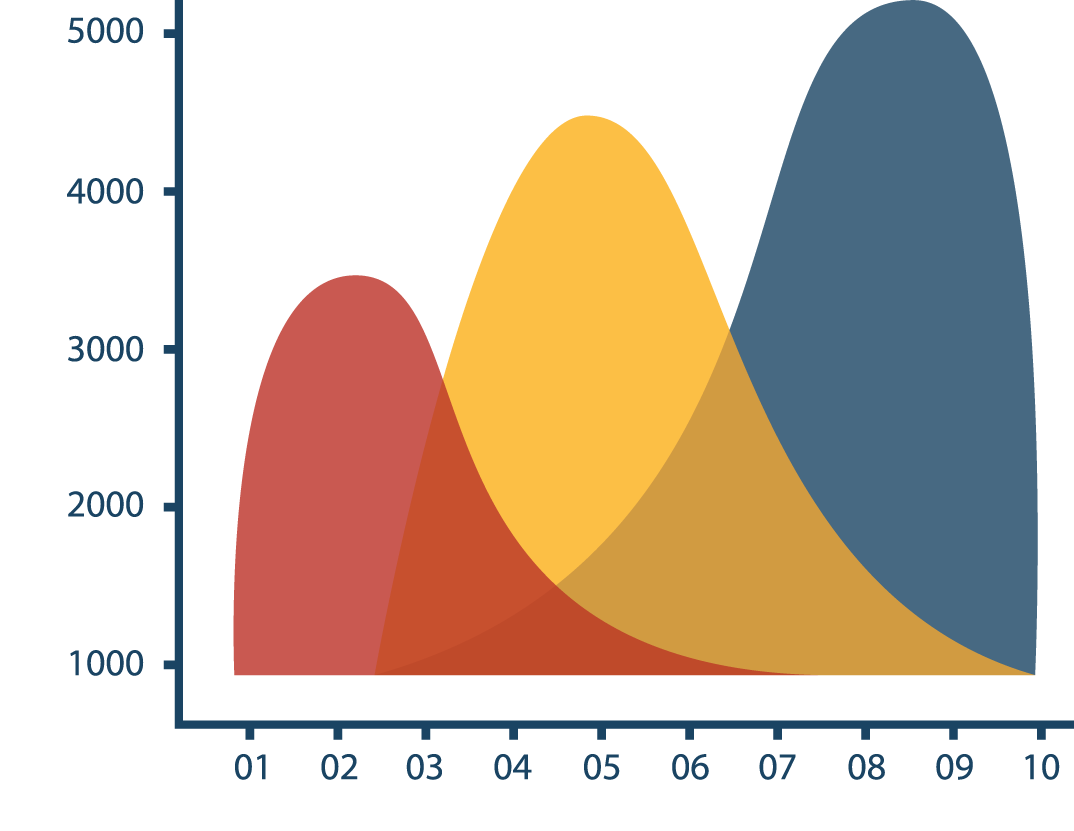
\includegraphics[width=0.5cm]{Figures/Graph.png} on the side of the \textbf{Projected Elemental Profiles} panel to view the discriminant scores (Fig.~\ref{fig:onevstherest-DFA-scatter}). The weight vector $\mathbf{w}$ (Eq.~\eqref{eq:discriminant_score}) is chosen to maximize the separation between the selected source group (Bank, in this example) and the remaining samples; the result window shows it in the \textit{Eigen vector} panel, one weight per constituent. Each sample's discriminant score, plotted in the figure, is the sum of its constituent values multiplied by these weights.

\begin{figure}[ht]
    \centering
    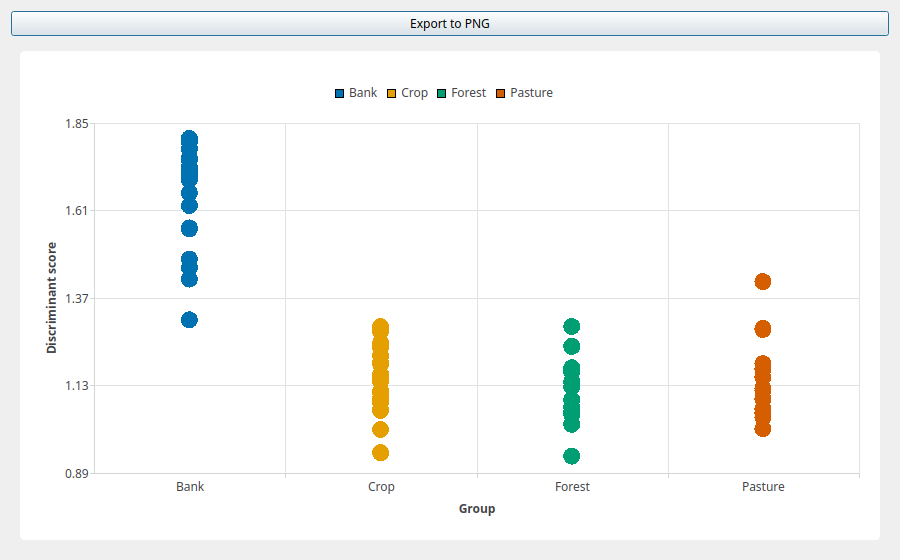
\includegraphics[width=\textwidth]{Figures/DFA_Scatter_onevstherest.png}
    \caption{Discriminant scores from one-vs-the-rest DFA for the Bank source group versus the rest, with the seven constituents selected in step~4 included.}
    \label{fig:onevstherest-DFA-scatter}
\end{figure}
\FloatBarrier

\section{Uncertainty and verification}\label{sec:tools-uncertainty}
\subsection{Error Analysis}\label{sec:tool-error}
The error analysis tool performs uncertainty analysis on the estimated source contributions by bootstrapping. In each realization, it randomly excludes a specified percentage of source samples and then re-estimates the source contributions using the Levenberg--Marquardt algorithm. The distribution of contributions across realizations gives a measure of how sensitive the inferred contributions are to the particular source samples used.

To perform error analysis, select \textbf{Tools}$\rightarrow$\textbf{Other Statistical Tools}$\rightarrow$\textbf{Uncertainty and verification}$\rightarrow$\textbf{Error Analysis} from the tools window. In the central form, choose the target sample, the number of realizations, and the percentage of source samples to exclude in each realization. You can also choose whether to run the analysis on source elemental profiles corrected for OM and particle size (for the target sample chosen), and enter a random seed (leave blank to have one chosen; the seed used is shown in the name of the results). Click \textbf{Ok}.

When the analysis is complete, the result window displays three panels.

The first panel shows the source contributions estimated for each realization. Click the table button~
\includegraphics[width=0.5cm]{Figures/table.png} next to the panel to view the inferred contributions in tabular form. If the number of realizations is fewer than 100, you can also view the results as a graph.

The second panel shows the frequency distribution of the inferred contributions across realizations. Click the graph button~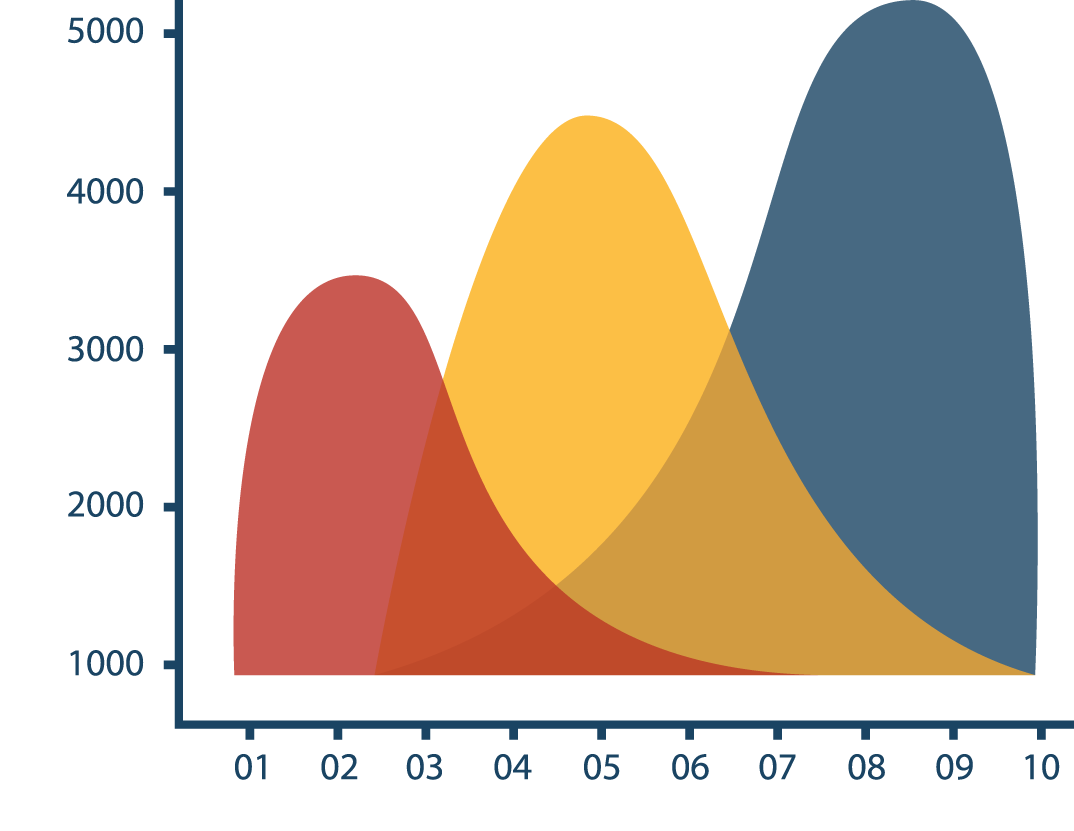
\includegraphics[width=0.5cm]{Figures/Graph.png} next to the panel to view the distribution for each source group (Fig.~\ref{fig:Error_analysis_results}). A narrow distribution means the contribution hardly depends on which source samples are used; a wide one, that it is sensitive to them.

\begin{figure}[ht]
    \centering
    \begin{tabular}{cc}
        a) & b) \\
        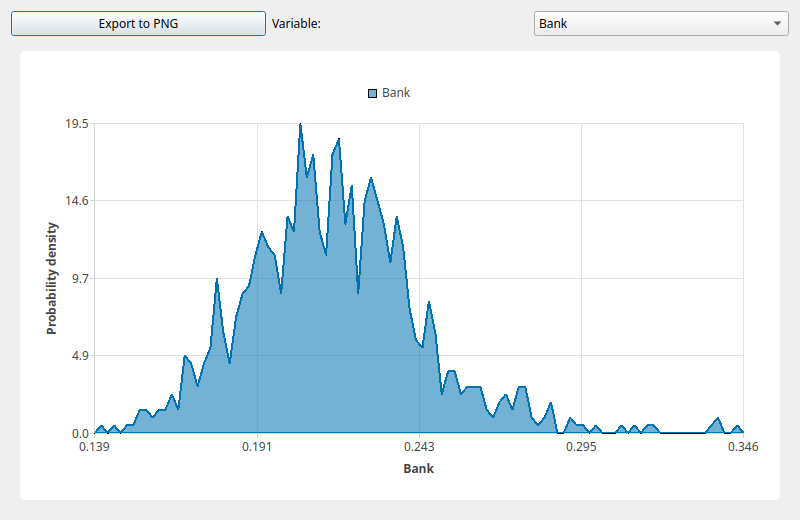
\includegraphics[width=0.46\textwidth]{Figures/Error_Analysis_Bank.png} &
        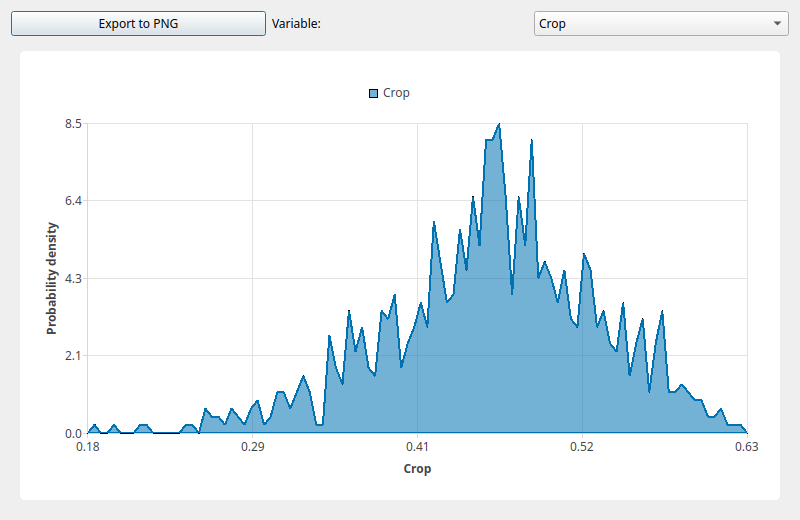
\includegraphics[width=0.46\textwidth]{Figures/Error_Analysis_crop.png} \\
        c) & d) \\
        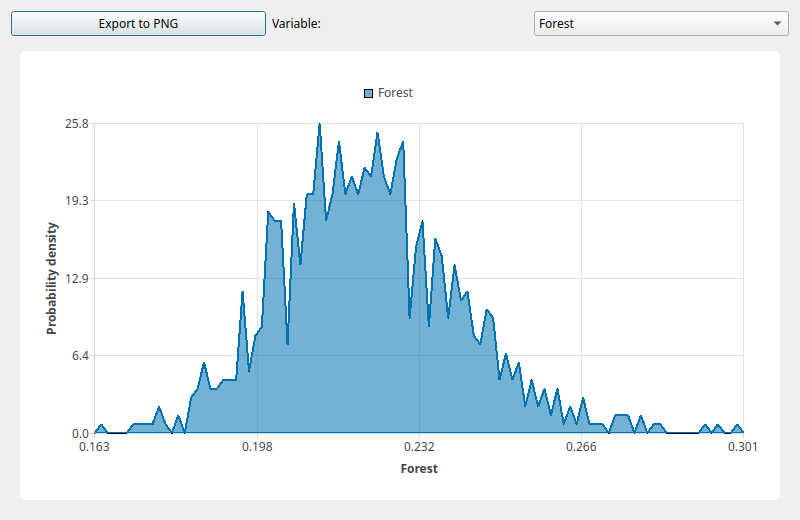
\includegraphics[width=0.46\textwidth]{Figures/Error_Analysis_forest.png} &
        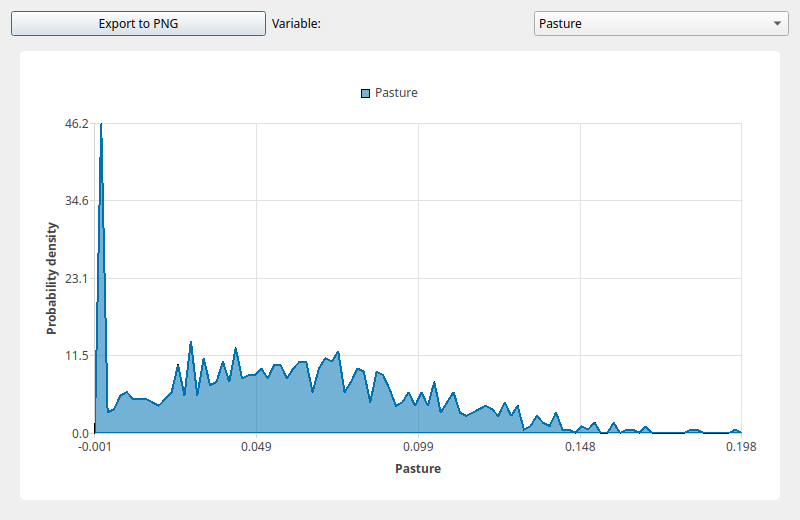
\includegraphics[width=0.46\textwidth]{Figures/Error_Analysis_pasture.png}
    \end{tabular}
    \caption{Frequency distributions of inferred source contributions from the error analysis for the a) Bank, b) Crop, c) Forest, and d) Pasture source groups.}
    \label{fig:Error_analysis_results}
\end{figure}
\FloatBarrier

The third panel contains the 95\% intervals of the source contributions across realizations. Click the graph button~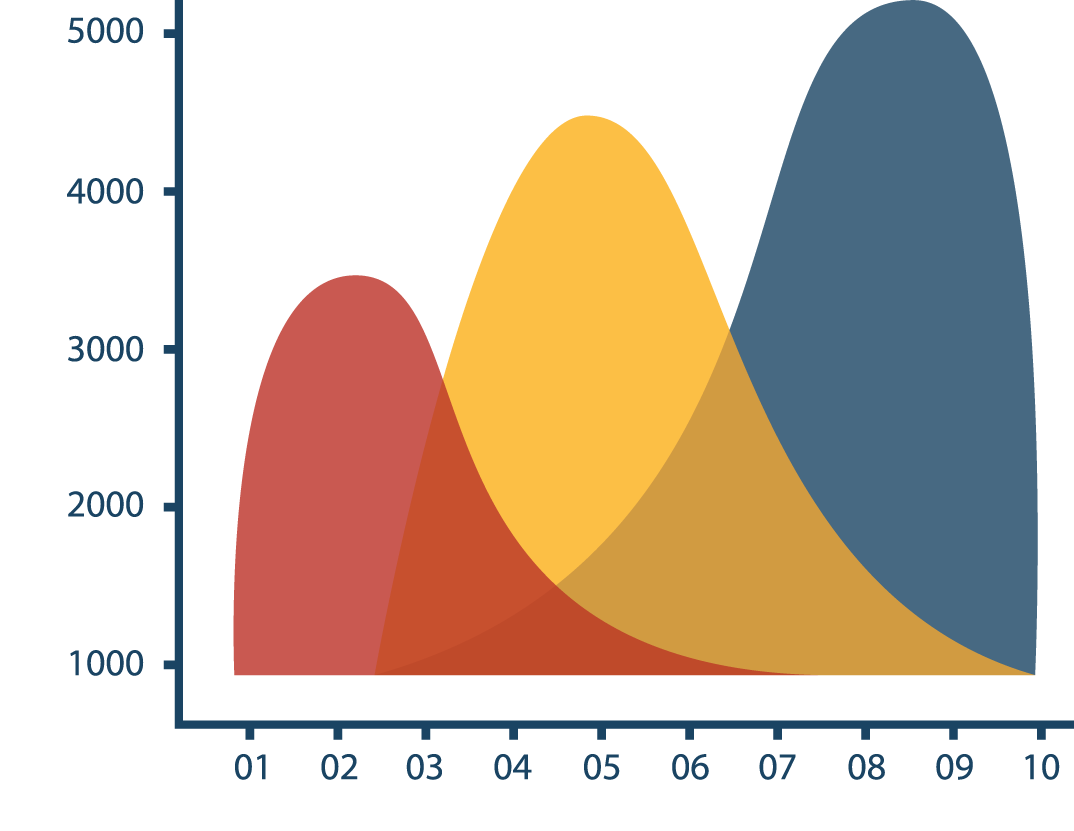
\includegraphics[width=0.5cm]{Figures/Graph.png} next to the panel to view them graphically (Fig.~\ref{fig:Error_Analysis_95_bound}): each green box spans the interval, and the line in it is the median.

\begin{figure}[ht]
    \centering
    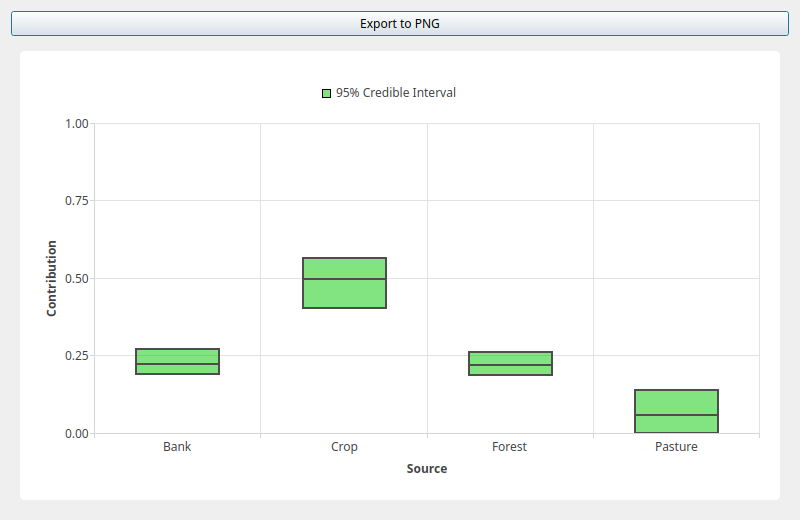
\includegraphics[width=0.46\textwidth]{Figures/Error_Analysis_CI.png}
    \caption{95\% bounds of the source contributions from the error analysis.}
    \label{fig:Error_Analysis_95_bound}
\end{figure}
\FloatBarrier

\subsection{Source Verification}\label{sec:tool-sourceverify}
The source verification tool assesses how well individual source samples align with their overall source group. It treats each source sample within a group as a target sample and performs fingerprinting using the Levenberg--Marquardt algorithm. If a source sample's elemental profile closely matches that of its source group, the analysis should identify that group as the dominant contributor.

To perform source verification, select \textbf{Tools}$\rightarrow$\textbf{Other Statistical Tools}$\rightarrow$\textbf{Uncertainty and verification}$\rightarrow$\textbf{Source Verification} from the tools window. In the central form, choose the source group on which to perform the analysis and whether to apply the size and organic matter correction. With the correction, the sources are corrected, for each source sample tested, to that sample's own organic matter content and particle size, as they would be for a target sample. Click \textbf{Ok}.

Source verification checks how well the selected tracers classify the source samples, as the confusion matrix of step~4 does (Section~\ref{sec:multiway-dfa}), but with the fingerprinting itself rather than the discriminant function: a sample attributed mostly to its own group is classified correctly, and one attributed mostly to another group is not. Running it for each source group shows which groups the tracers confuse.

\begin{tcolorbox}[colback=yellow!10,colframe=yellow!50!black,title=Note]
Only the elements and samples marked for inclusion in \textbf{Settings}$\rightarrow$\textbf{Constituent Properties} and \textbf{Settings}$\rightarrow$\textbf{Include/Exclude Samples} are considered in the analysis.
\end{tcolorbox}

The result window shows the estimated contribution of each source group to each sample in the selected source group. Click the table button~
\includegraphics[width=0.5cm]{Figures/table.png} or the graph button~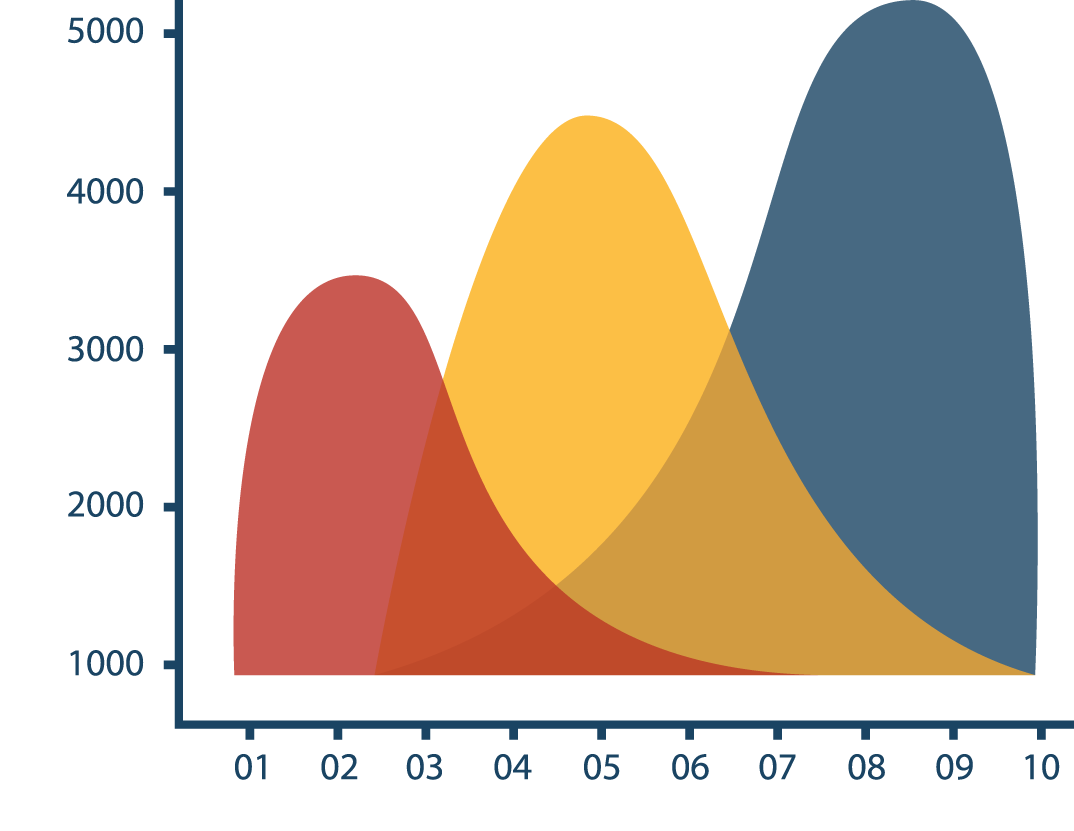
\includegraphics[width=0.5cm]{Figures/Graph.png} to view the results in tabular or graphical form (Fig.~\ref{fig:source_verification}).

\begin{figure}[ht]
    \centering
    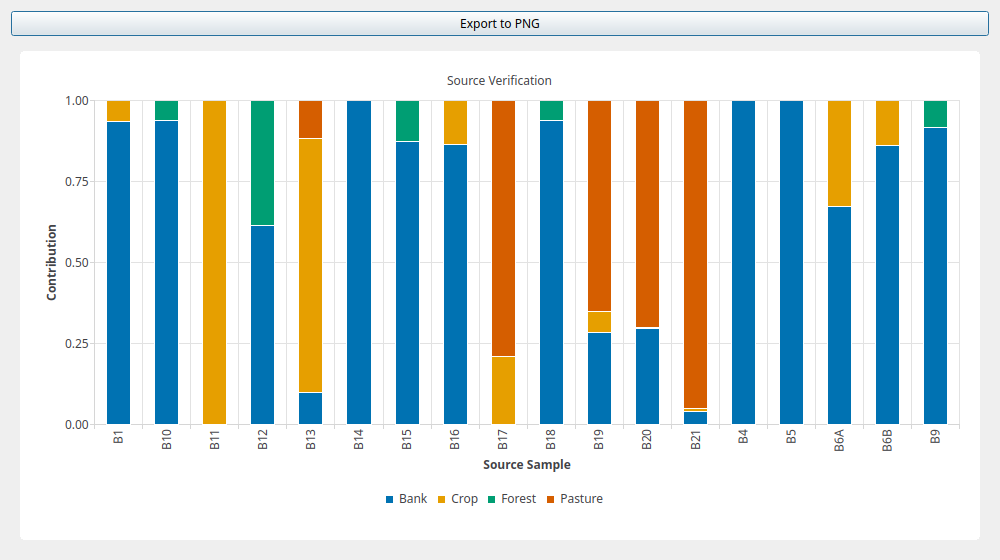
\includegraphics[width=\textwidth]{Figures/Source_verify_graph.png}
    \caption{Source verification results: estimated contribution of each source group to each sample within the selected source group.}
    \label{fig:source_verification}
\end{figure}
\FloatBarrier

\section{Genetic Algorithm estimation (not in this release)}
\begin{tcolorbox}[colback=yellow!10,colframe=yellow!50!black,title=Note]
The genetic algorithm is not part of this release of SedSAT3 and does not appear in the \textbf{Tools} menu: the Levenberg--Marquardt method solves the same problem more efficiently. The method is described here for completeness; it is available only in a build made with the genetic algorithm option.
\end{tcolorbox}

The genetic algorithm (GA) estimation method does not compute the mean elemental profile of each source group directly from the source samples; instead, it estimates the mean of each constituent in each source as part of the inverse modeling. Each constituent in each source group is assumed to follow a log-normal distribution:
\begin{equation}
    \tilde{y}_{i,j} \sim \frac{1}{\sqrt{2\pi}\,\sigma_j\, y_{i,j}} \exp\left(-\frac{[\ln(y_{i,j}) - \mu_{i,j}]^2}{2\sigma_j^2}\right)
\end{equation}
where $\sigma_j$ is the shape parameter of the log-normal distribution for element $j$, assumed to be the same for all source groups, and $\mu_{i,j}$ is the scale parameter. The values of $\sigma_j$ and $\mu_{i,j}$ are estimated jointly with the source contributions. For a given set of $\sigma$, $\mu$, and source contribution values, the mean elemental profile of each source is computed from the parameters of the log-normal distribution as:
\begin{equation}
    y_{i,j} = \exp\left(\mu_{i,j} + \frac{\sigma_j^2}{2}\right)
\end{equation}

Because the number of parameters to be estimated is much larger here than in the case where the mean elemental profiles are calculated directly from the source samples, SedSAT3 uses a genetic algorithm for the optimization. An optional hybrid mode combines a conventional binary genetic algorithm with a stochastic gradient descent step \citep{alikhani2017evaluation}.

In a build with the genetic algorithm, the settings of the GA fingerprinting form are:

\begin{itemize}
    \item \textbf{Apply size and organic matter correction:} whether to run the analysis on elemental profiles corrected for size and organic matter. The size and organic matter correction step (Section~\ref{sec:sizeandorganiccorrection}) must have been performed beforehand.
    \item \textbf{Sample:} the target sample to be analyzed.
    \item \textbf{Population:} the number of individuals in each GA generation. Increase this value if the GA does not converge with the default; 100 is usually adequate.
    \item \textbf{Number of Generations:} the number of generations run by the GA. Increase this value if convergence has not been reached.
    \item \textbf{Crossover probability:} the probability of crossover in the GA. The default value of 1.0 is usually appropriate.
    \item \textbf{Mutation probability:} the probability of mutation in the GA. The default value is usually appropriate.
    \item \textbf{Numerical crossover:} when checked, the algorithm uses a numerical crossover operator rather than a binary one.
    \item \textbf{Shake coefficient:} the magnitude of the numerical perturbation applied when the GA fails to improve the likelihood over several consecutive generations. Leave at the default value.
    \item \textbf{Shake coefficient reduction factor:} the factor by which the shake coefficient is reduced if the likelihood does not improve after several consecutive shaking iterations.
    \item \textbf{Gradient Descent:} when checked, combines the genetic algorithm with a gradient descent step, often resulting in faster and more accurate convergence.
    \item \textbf{Number of threads used:} the number of processor threads used for the GA optimization. If the value exceeds the number of CPU cores available, all cores are used.
    \item \textbf{GA output file:} the text file in which detailed information about the GA process is saved.
\end{itemize}

\begin{tcolorbox}[colback=yellow!10,colframe=yellow!50!black,title=Note]
The GA is not guaranteed to find the global optimum within a given number of generations. As a check, run the fingerprinting multiple times to verify that the inferred contributions are consistent, or increase the number of generations and check whether the results change. Substantial run-to-run variation may indicate equifinality, in which several distinct source combinations produce similarly good fits to the target sample.
\end{tcolorbox}

After setting the parameters, click \textbf{Ok} and wait for the analysis to complete. The result window contains nine panels:

\begin{enumerate}
    \item \textbf{Inferred source contributions} --- click the graph button~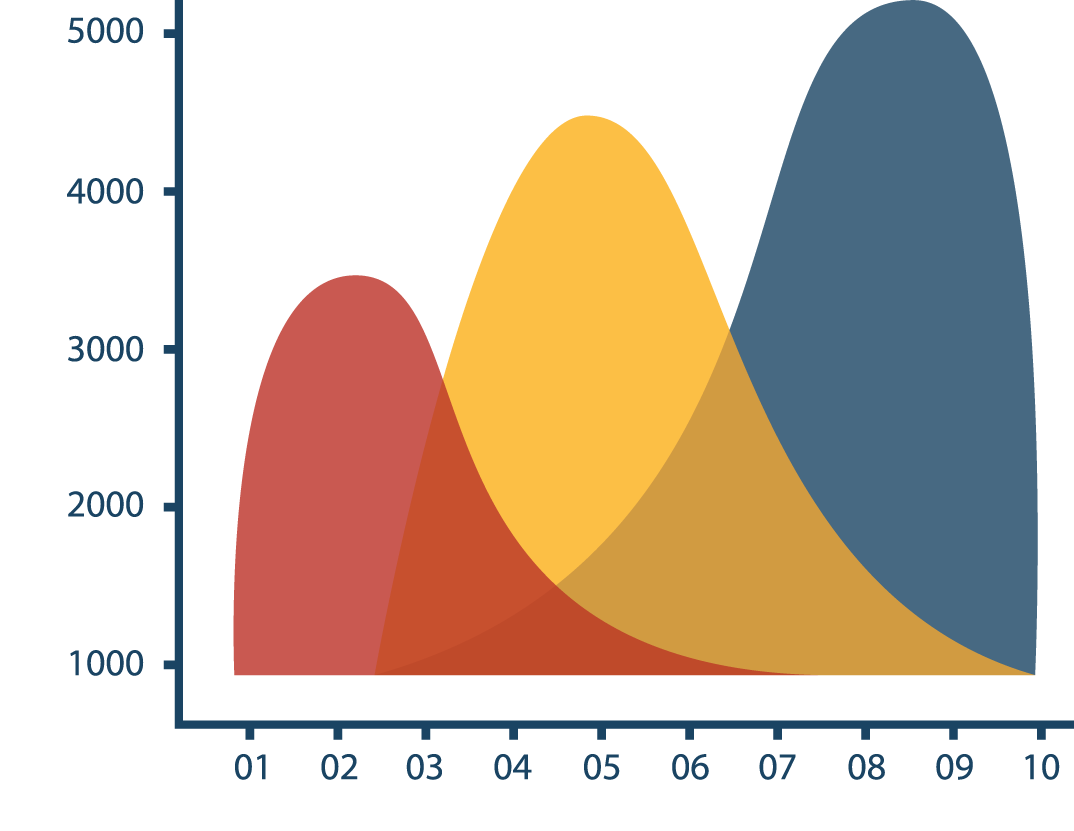
\includegraphics[width=0.5cm]{Figures/Graph.png} to view the contributions as a pie chart (Fig.~\ref{fig:GA-contribution}).

    \begin{figure}[ht]
        \centering
        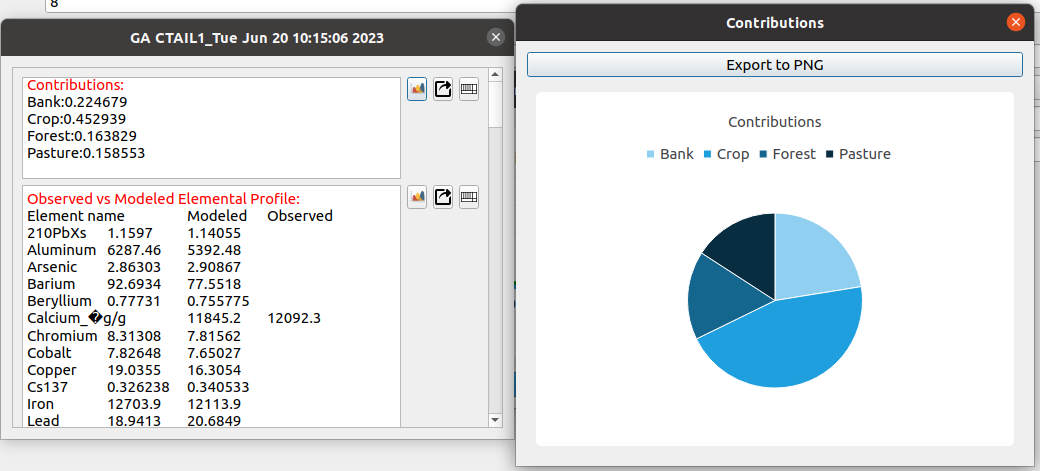
\includegraphics[width=\textwidth]{Figures/GA_Contributions.png}
        \caption{Estimated source contributions from the genetic algorithm.}
        \label{fig:GA-contribution}
    \end{figure}
    \FloatBarrier

    \item \textbf{Modeled vs.\ measured elemental contents} (Fig.~\ref{fig:GA-modeledvsobserved}).

    \begin{figure}[ht]
        \centering
        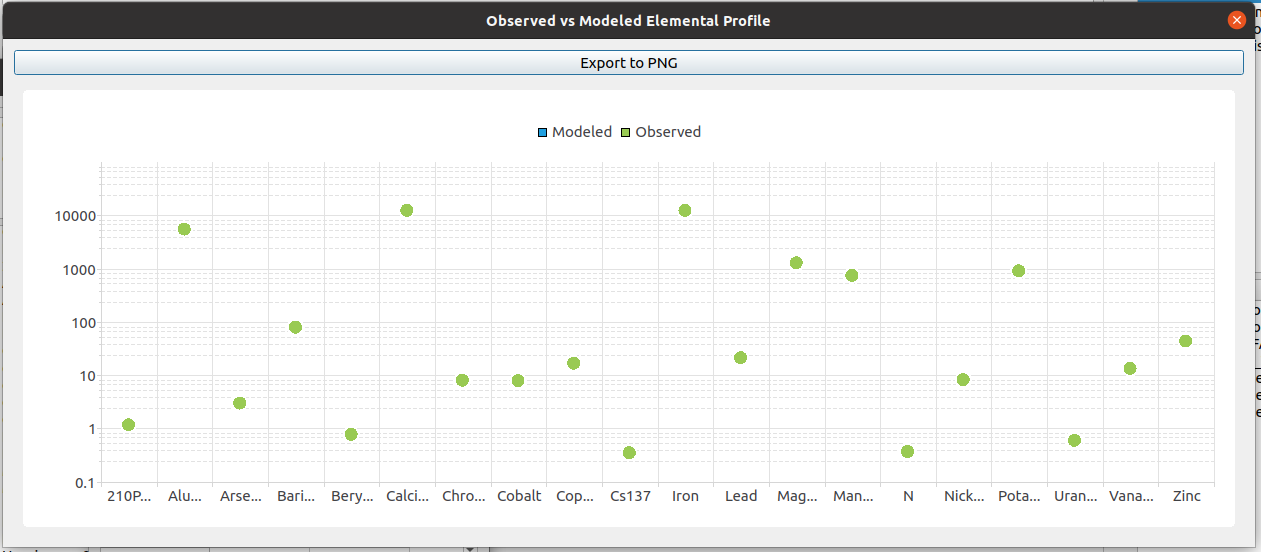
\includegraphics[width=\textwidth]{Figures/GA-Modeled_vs_measured_graph.png}
        \caption{Modeled vs.\ measured elemental contents from the genetic algorithm.}
        \label{fig:GA-modeledvsobserved}
    \end{figure}
    \FloatBarrier

    \item \textbf{Modeled vs.\ measured isotope $\delta$ values}, shown when isotopes are included in the analysis.
    \item \textbf{Calculated element means} for each source group, computed directly from the source samples.
    \item \textbf{Estimated element means} based on the estimated log-normal distribution parameters.
    \item \textbf{Calculated scale parameter $\mu$} of the log-normal distribution for each element in each source, computed from the geometric mean of the source-sample elemental contents.
    \item \textbf{Estimated scale parameter $\mu$} from the genetic algorithm.
    \item \textbf{Calculated shape parameter $\sigma$} of the log-normal distribution for each element, computed from the source samples.
    \item \textbf{Estimated shape parameter $\sigma$} from the genetic algorithm.
\end{enumerate}

Panels 4--5 and 6--9 are particularly useful for diagnosing the results: large discrepancies between the calculated values (computed directly from the source samples) and the estimated values (recovered by the GA) may indicate convergence problems or model misfit.

\chapter{Mathematical Basis}\label{sec:basic_concepts}

\section{Mass balance formulation}
The basis of sediment fingerprinting is the use of tracer groups (each representing a distinct sediment source) to identify statistically significant differences in chemical properties between the source areas and the fluvial sediments (the target sample). If $n$ sources are mixed and $y_{i,j}$ [M/M] is the mass fraction of element $j$ in source $i$, the content of element $j$ in the mixture (the target sample) is:
\begin{equation}\label{eq:sum}
    c_j = \sum_i x_i y_{i,j}
\end{equation}
where $x_i$ is the contribution fraction of source $i$. Equation~\eqref{eq:sum} can be written for all elements in the analysis in matrix form:
\begin{equation}\label{eq:mass_balance_matrix}
    \mathbf{C} = \mathbf{Y} \mathbf{X}
\end{equation}
where $\mathbf{C}_{m} = [\dots\, c_j\, \dots]^T$ is the vector containing the target sample elemental profile, $\mathbf{X}_{n} = [\dots\, x_i\, \dots]^T$ is the vector of source contribution fractions, $\mathbf{Y}_{n \times m} = [y_{i,j}]$ is the matrix of source elemental contents, and $m$ is the number of elements (or signatures) included in the analysis.

The contribution fractions must sum to one:
\begin{equation}\label{eq:sum_constraint}
    \sum_i x_i = 1
\end{equation}

\subsection{Stable isotopes}\label{sec:stable-isotopes}
Stable isotopes are also commonly used for sediment fingerprinting. The stable isotope content of a sample is conventionally expressed using the $\delta$ value:
\begin{equation}\label{eq:delta_def}
    \delta\,{}^{u}E = \left(\frac{{}^{u}E/E}{\left({}^{u}E/E\right)_{\mathrm{std}}} - 1\right) \times 1000
\end{equation}
where ${}^{u}E$ is the isotope content and $E$ is the base element content. The quantity $\left({}^{u}E/E\right)_{\mathrm{std}}$ is a standard isotope ratio used as the reference for the $\delta$ value. Solving Eq.~\eqref{eq:delta_def} for ${}^{u}E$ gives:
\begin{equation}\label{eq:isotope_content}
    {}^{u}E = \left(\frac{\delta\,{}^{u}E}{1000} + 1\right) \left({}^{u}E/E\right)_{\mathrm{std}} E
\end{equation}

When several sediment sources are mixed, the isotope content of the mixture is:
\begin{equation}\label{eq:isotope_mass_balance}
    \zeta_j = \sum_i x_i \upsilon_{i,j}
\end{equation}
where $\zeta_j$ is the content of isotope $j$ in the mixture and $\upsilon_{i,j}$ is the mean content of isotope $j$ in source $i$, calculated via Eq.~\eqref{eq:isotope_content}.

Substituting Eq.~\eqref{eq:isotope_content} into Eq.~\eqref{eq:isotope_mass_balance} yields the mixture $\delta$ value:
\begin{equation}\label{eq:delta_mixture}
    \delta\zeta_j = \frac{\sum_i x_i\, \delta\upsilon_{i,j}\, y_{i,j}}{\sum_i x_i\, y_{i,j}}
\end{equation}
where $\delta\upsilon_{i,j}$ is the $\delta$ value of isotope $j$ in source $i$.

The set of equations obtained from isotopes can be appended to Eq.~\eqref{eq:mass_balance_matrix}. Note that to include an isotope in the analysis, the base element of that isotope must also be measured. The base element can be a tracer included in the analysis or, for $\delta^{13}$C, the organic carbon content (TOC), which is then used only through Eq.~\eqref{eq:delta_mixture}: the mixture's base content is $\sum_i x_i y_{i,j}$, with $y_{i,j}$ the mean base content of source $i$.

$\delta$ values are commonly negative (for example $\delta^{13}$C of organic matter) and can be both positive and negative within one dataset (for example $\delta^{15}$N). SedSAT3 handles this as follows. The isotope content computed by Eq.~\eqref{eq:isotope_content} is positive for any $\delta$ above $-1000$, so the mass balance (Eqs.~\ref{eq:isotope_mass_balance} and~\ref{eq:delta_mixture}) is valid for negative and mixed-sign $\delta$ values. In the likelihood, the residuals of isotopes are differences of $\delta$ values on a linear scale, while those of elements are differences of logarithms (Section~\ref{sec:mle}). $\delta$ values are therefore never log-transformed. Operations that need positive values are not applied to them: the Box--Cox transformation leaves them untransformed ($\lambda = 1$), and a log-normal distribution cannot be fitted to them.

\section{Maximum likelihood estimation}\label{sec:mle}
The goal of sediment fingerprint modeling is to estimate the source contributions $\mathbf{X}$ given measurements of the elemental profiles of a number of source groups, $\mathbf{Y}$, and the elemental profile of the target sample, $\mathbf{C}$. We denote the measured source elemental profiles by $\tilde{\mathbf{Y}}$ and the measured target sample profile by $\tilde{\mathbf{C}}$. The goal is then to infer $\mathbf{X}$ given $\tilde{\mathbf{Y}}$ and $\tilde{\mathbf{C}}$. Because multiple samples typically represent each source group, there are multiple instances of $\tilde{\mathbf{Y}}$; we denote the elemental profile of source sample $k$ by $\tilde{\mathbf{Y}}_k$.

\subsection{Treating source elemental composition deterministically}
The simplest assumption is that $\mathbf{Y}$ is known deterministically as the arithmetic average over all samples representing each source group:
\begin{equation}\label{eq:y_avg}
    y_{i,j} = \frac{1}{ns_i} \sum_k \tilde{y}_{i,j,k}
\end{equation}
where $ns_i$ is the number of samples in source group $i$.

Assuming conditional independence of errors, the probability density of observing the measured target elemental profile $\tilde{\mathbf{C}}$ given a contribution vector $\mathbf{X}$ is:
\begin{equation}\label{eq:likelihood_C_given_X}
    p(\tilde{\mathbf{C}} \mid \mathbf{X}) = \prod_j \frac{g'_j(\tilde{c}_j)}{\sigma_j} \phi\!\left(\frac{g_j[c_j(\mathbf{X})] - g_j(\tilde{c}_j)}{\sigma_j}\right)
\end{equation}
where $\phi$ is the standard normal density, $\sigma_j$ is the error standard deviation for element $j$, and $g_j$ is a transformation function chosen to map the error distribution onto a normal distribution. The choice of $g_j$ determines the assumed error structure: $g_j(c_j) = c_j$ yields a Gaussian likelihood (additive errors), while $g_j(c_j) = \ln(c_j)$ yields a log-normal likelihood (multiplicative errors).

The log-likelihood is typically used for maximum likelihood estimation:
\begin{equation}\label{eq:loglikelihood}
    \ln p(\tilde{\mathbf{C}} \mid \mathbf{X}) = \sum_j \ln g'_j(\tilde{c}_j) - \sum_j \ln \sigma_j - \frac{m}{2}\ln \pi - \sum_j \frac{\{g_j[c_j(\mathbf{X})] - g_j(\tilde{c}_j)\}^2}{2\sigma_j^2}
\end{equation}
Because the first three terms are independent of $\mathbf{X}$, maximizing the log-likelihood is equivalent to maximizing the last term, which is a least-squares problem in the transformed space. An optimization algorithm can be used to estimate both $\mathbf{X}$ and the $\sigma_j$ values that maximize the log-likelihood.

If the error structure is log-normal and multiplicative, it is often reasonable to assume that the error standard deviation $\sigma$ is the same for all elements (i.e., the expected relative error is the same for all elements). Under this assumption, Eq.~\eqref{eq:loglikelihood} simplifies to:
\begin{equation}\label{eq:loglikelihood-eqstd}
    \ln p(\tilde{\mathbf{C}} \mid \mathbf{X}) = \sum_j \ln g'_j(\tilde{c}_j) - m \ln \sigma - \frac{m}{2}\ln \pi - \frac{1}{2\sigma^2} \sum_j \{g_j[c_j(\mathbf{X})] - g_j(\tilde{c}_j)\}^2
\end{equation}
so that estimating $\mathbf{X}$ reduces to minimizing the sum of squared errors $\sum_j \{g_j[c_j(\mathbf{X})] - g_j(\tilde{c}_j)\}^2$.

\subsection{Treating source elemental composition as unknown}
Because the number of samples collected per source is typically limited, the estimate of $\mathbf{Y}$ obtained from Eq.~\eqref{eq:y_avg} may not be accurate. We can instead assume that the elemental content of each source follows a probability distribution:
\begin{equation}
    \tilde{y}_{i,j} \sim p_{y,i,j}(\bm{\theta}_{i,j})
\end{equation}
or, in matrix form:
\begin{equation}
    \mathbf{Y} \sim \mathbf{P}_y(\bm{\Theta})
\end{equation}
where $\bm{\theta}_{i,j}$ is the parameter vector of the distribution for element $j$ in source $i$, $\bm{\Theta}$ collects all such parameters across elements and sources, and $\mathbf{P}_y$ denotes the joint distribution of all elemental contents in all sources.

For maximum likelihood estimation in this case, the joint probability of observing the target elemental profile and the source elemental profiles of all samples should be maximized:
\begin{equation}\label{eq:loglikelihood-with-y}
    p(\tilde{\mathbf{C}}, \tilde{\mathbf{Y}} \mid \mathbf{X}, \mathbf{Y}) = \prod_j \frac{g'_j(\tilde{c}_j)}{\sigma_j} \phi\!\left(\frac{g_j[c_j(\mathbf{X}, \bm{\Theta})] - g_j(\tilde{c}_j)}{\sigma_j}\right) \prod_k \mathbf{P}_y(\tilde{\mathbf{Y}}_k;\, \bm{\Theta})
\end{equation}
where $\tilde{\mathbf{Y}}_k$ is the observed source elemental matrix for sample $k$. Because the expected value of $\mathbf{P}_y$ depends on its parameters $\bm{\Theta}$, the predicted target elemental profile depends jointly on the source contributions and the source distribution parameters:
\begin{equation}\label{eq:c_with_theta}
    c_j(\mathbf{X}, \bm{\Theta}) = \sum_i x_i\, E(y_{i,j};\, \bm{\theta}_{i,j})
\end{equation}
where $E(y_{i,j};\, \bm{\theta}_{i,j})$ is the expected value of $y_{i,j}$ under the source elemental content distribution:
\begin{equation}
    E(y;\, \bm{\theta}) = \int y\, p_y(y;\, \bm{\theta})\, \mathrm{d}y
\end{equation}

For example, if $p_y$ is a log-normal distribution with parameters $\bm{\theta} \equiv \{\mu, \sigma\}$, then $E(y) = \exp(\mu + \sigma^2/2)$.

Assuming the distributions of elemental contents in different sources are independent, the log-likelihood is obtained by taking the logarithm of Eq.~\eqref{eq:loglikelihood-with-y}:
\begin{equation}
\begin{split}
    \ln p(\tilde{\mathbf{C}}, \tilde{\mathbf{Y}} \mid \mathbf{X}, \mathbf{Y}) = \sum_j \ln g'_j(\tilde{c}_j) &- \sum_j \ln \sigma_j - \frac{m}{2}\ln \pi \\
    &- \sum_j \frac{\{g_j[c_j(\mathbf{X}, \bm{\Theta})] - g_j(\tilde{c}_j)\}^2}{2\sigma_j^2} \\
    &+ \sum_i \sum_j \sum_k \ln p_{y,i,j}(\tilde{y}_{i,j,k};\, \bm{\theta}_{i,j})
\end{split}
\end{equation}
Because the first three terms are independent of $\mathbf{X}$ and $\bm{\Theta}$, the optimization reduces to maximizing the last two terms.

\section{Bayesian inference}\label{sec:basic_concepts_bayesian}
Sediment fingerprinting is subject to several sources of uncertainty, including measurement errors in both target and source samples, non-uniform selection or release of source material, model structural errors arising from changes in elemental composition during transport, the presence of unmodeled sources, and equifinality.

Measurement errors are an unavoidable part of chemical analysis and can also arise from the natural variability of sediment characteristics. Non-uniform source selection occurs when the elemental profile of a source varies systematically across space, so that the distribution of material actually mobilized from a source differs from the distribution obtained from a spatially uniform sampling of that source. Structural errors arise because the model is a simplification of the real processes; for example, changes in elemental composition during transport can introduce model structural error. Some sediment sources may not be included in the analysis at all, leading to inaccuracies in the inferred contributions. Equifinality refers to the situation in which multiple source combinations produce equally good matches to the target sample, making it difficult to identify the true source mixture uniquely.

Quantifying these uncertainties is essential for making sound engineering or management decisions based on sediment fingerprinting results. In contrast to maximum likelihood approaches, which produce point estimates, Bayesian inference yields a joint probability distribution over the inferred parameters.

Bayesian inference is based on Bayes' theorem:
\begin{equation}\label{eq:Bayesian}
    p(\bm{\Upsilon} \mid \bm{\Xi}) = \frac{p(\bm{\Xi} \mid \bm{\Upsilon})\, p(\bm{\Upsilon})}{p(\bm{\Xi})}
\end{equation}
where $\bm{\Upsilon}$ denotes the model parameters, $\bm{\Xi}$ denotes the observed data, $p(\bm{\Xi} \mid \bm{\Upsilon})$ is the likelihood, $p(\bm{\Upsilon})$ is the prior distribution of the parameters, and $p(\bm{\Xi})$ is a normalizing constant ensuring that the posterior distribution $p(\bm{\Upsilon} \mid \bm{\Xi})$ integrates to one. For all but the simplest problems, the posterior cannot be evaluated analytically, and methods such as Markov chain Monte Carlo (MCMC) are used to draw a large number of samples from it. MCMC does not require the absolute value of the posterior density; it requires only the ratio of densities at any two parameter values. Because the denominator in Eq.~\eqref{eq:Bayesian} is independent of $\bm{\Upsilon}$, it can be omitted, yielding the proportionality:
\begin{equation}\label{eq:Bayesian-Prop}
    p(\bm{\Upsilon} \mid \bm{\Xi}) \propto p(\bm{\Xi} \mid \bm{\Upsilon})\, p(\bm{\Upsilon})
\end{equation}

In the context of sediment fingerprinting, Eq.~\eqref{eq:Bayesian-Prop} becomes:
\begin{equation}\label{eq:Bayesian-Sediment}
    p(\mathbf{X}, \mathbf{Y} \mid \tilde{\mathbf{C}}, \tilde{\mathbf{Y}}) \propto p(\tilde{\mathbf{C}}, \tilde{\mathbf{Y}} \mid \mathbf{X}, \mathbf{Y})\, p(\mathbf{X})\, p(\mathbf{Y})
\end{equation}
where $p(\mathbf{X})$ is the prior on source contributions and $p(\mathbf{Y})$ is the prior on the source elemental profiles. In the absence of additional information, a reasonable choice is to set $p(\mathbf{X})$ to a symmetric Dirichlet distribution with concentration parameter $\alpha = 1$ (which is the uniform distribution over the simplex). The prior $p(\mathbf{Y})$ is taken to be non-informative, since $\mathbf{Y}$ is already constrained by the likelihood through the source-sample observations. The likelihood $p(\tilde{\mathbf{C}}, \tilde{\mathbf{Y}} \mid \mathbf{X}, \mathbf{Y})$ is computed from Eq.~\eqref{eq:loglikelihood-with-y}.

\section{Summary}
SedSAT3 estimates the contributions of sediment sources to a target sample from a mass balance of elements and isotopes (Section~\ref{sec:basic_concepts}). The maximum likelihood method (Levenberg--Marquardt) finds the single combination of source contributions that best explains the measured target sample. Bayesian inference describes the uncertainty of the contributions with a joint probability distribution, sampled by MCMC, which accounts for the variability of the source samples and the error of the measurements. The pre-analysis tools of Chapters~\ref{chap:deterministic} and~\ref{chap:other-tools} prepare the data so that the assumptions of these models hold as closely as possible: conservative tracers that bracket the target sample, source groups that the tracers distinguish, and source data comparable with the target in organic matter content and particle size.



\bibliography{references.bib}


\end{document}
